In questa capitolo verranno valutate le performance dell'algoritmo RePBubLik+, confrontadolo
con altri due algoritmi noti per la riduzione della polarizzazione dei grafi: ROV e Node2Vec.

\section{Algoritmi confrontati}
\subsection{ROV(Recommend Opposing View)}
L'algoritmo ROV\cite{ROV} fornisce come output un insieme di $k$ archi da aggiungere a $G$ per minimizzare
il controversy score (Random Walk Controversy). Questa è una metrica che caratterizza quanto un topic
è ``controverso'', cioè quanto è ben separato rispetto agli altri topic. L'algoritmo ROV prende come 
archi candidati quelli che collegano i vertici ad alto grado (con molti archi incidenti) di ciascun "colore"
(topic). Gli archi vengono ordinati in ordine decrescente in funzione del loro impatto sul RWC nel grafo, 
e di questi si individuano i migliori $k$ da aggiungere al grafo G.

\subsection{Node2Vec}
L'algoritmo Node2Vec\cite{Node2Vec} permette di rappresentare un grafo in uno spazio vettoriale a bassa dimensionalità, mantenendo
inalterate alcune caratteristiche importanti della rete come, ad esempio, la similiarità tra nodi.
La generazione di questo spazio vettoriale si basa sui random walk del grafo. Sullo spazio generato,
vengono generalmente eseguiti e addestrati algoritmi di raccomandazione di link. Questo processo permette
di migliorare il suggerimento di nuovi collegamenti all'interno del grafo.
\\
Nell' esperimento svolto, per ogni grafo, viene generato uno spazio a 128 dimensioni e, su quest'ultimo, verrà addestrato
un algoritmo di regressione logistica. Successivamente, verrà predetta la probabilità di esistenza di ciascun arco uscente da $P(G)$.
Al termine, verranno scelti i migliori $k$ archi da aggiungere al grafo $G$, in funzione della loro probabilità.

\section{Dataset}
Nelle analisi, vengono generati grafi dai dataset di \href{https://snap.stanford.edu/data/amazon-meta.html}{Amazon} e \href{http://www-personal.umich.edu/~mejn/netdata/}{PolBlogs}.
%Tabella riassuntiva caratteristiche
\begin{itemize}
\item Il dataset di Amazon contiene informazioni sui libri venduti. Ogni libro è un vertice e 
appartiene ad una categoria (ad un ``colore''). Esiste un arco diretto $(u,v)$ nel grafo se $v$ appartiene alla lista di 
libri simili a $u$ e il suo peso è determinato dal ``sales rank'' di $v$. Da questo dataset, si ottengono tre grafi formati
dalle seguenti coppie di categorie: \emph{Mathematics - Technology}(MaTe), \emph{History of Technology - Military Science}(MiHi) e
\emph{Mathematics - Astronomy }(MaAs).  
\item Il dataset di PolBlogs è una rete diretta di link tra weblogs sulla politica americana. Ogni nodo rappresenta un blog ed è 
``colorato'' in funzione del suo orientamento politico. I link tra i blogs (gli archi nel nostro grafo) sono estratti automaticamente 
da una scansione della pagina principale dei blog. Il peso di un arco $(v,u)$ è dato dal numero di archi uscenti dal vertice $v$.
\end{itemize}
Di seguito una tabella riassuntiva delle statistiche dei grafi generati.
\begin{table}[!h]
    \centering
    \begin{tabular}{lcccccccc}
        \hline
        \multicolumn{9}{c}{\emph{Amazon}} \\
        Topic    & $|V|$ &  $|R|$ & $|B|$ & $|E|$ &  $|E|_{R \to B}$ & $|E|_{B \to R}$ & $\%P_R(G)$ & $\%P_B(G)$\\
        \hline
        \emph{MaTe} & 1393 & 827 & 566 & 675 & 25 & 42 &  90.91 & 79.63\\
        \emph{MiHi} & 851 & 446 & 405 & 482 & 66 & 63 &  58.33 & 63.46\\
        \emph{MaAs} & 1121 &827 & 294 & 680 & 11 & 6 &  97.31 & 95.15\\
        \hline
        \multicolumn{9}{c}{\emph{PolBlogs}} \\
        Topic    & $|V|$ & $|R|$ & $|B|$ & $|E|$ & $|E|_{R \to B}$ & $|E|_{B \to R}$ & $\%P_R(G)$ & $\%P_B(G)$\\
        \hline
        \emph{PolBlogs} & 1033 & 545 & 488 & 17348 & 902 & 781 &  87.71 & 90.37\\
        \hline
    \end{tabular}
    \caption{Tabella delle statisiche dei grafi.
    La colonna $|V|$ specifica il numero di vertici appartenenti al grafo corrispondente.
    Le colonne $|R|$ e $|B|$ indicano, rispettivamente, il numero di vertici di colore $R$ e $B$. 
    La colonna $|E|$ indica il numero di archi del grafo corrispondente.
    Le colonne $|E|_{B \to R}$ e $|E|_{R \to B}$ specificano, rispettivamente, il numero di archi che vanno da nodi di colore $R$ a $B$ e  il numero di archi che vanno da nodi di colore $B$ a $R$.
    Le colonne $\%P_{R}(G)$ e $\%P_{R}(G)$ specificano la percentuale di nodi parochial del grafo $G$ rispettivamente di colore $R$ e $B$.}
\end{table} 
\section{Parametri dei test}
Per ogni grafo, sono stati eseguiti gli algoritmi RePBubLik+, ROV e Node2Vec, con valori crescenti
di $K$ (numero di archi da aggiungere) e con valori di $t$, ovvero la lunghezza massima dei random walk. 
Il valore massimo di $K$ è stato assegnato a 400, per tutti e quattro i grafi in esame.
Da notare che, per come è stato ideato lo script degli algoritmi, il numero finale di archi aggiunti
può essere ben inferiore al numero $K$ impostato manualmente. Per ogni grafo, infatti, vengono allocati $k_B$ archi per il colore $B$ e $k_R$ archi 
per il colore $R$, in proporzione alla somma dei Bubble Radius dei vertici parochial di ciascun colore.
Questo metrica permette di aggiungere più archi per il colore avente più vertici parochial.
Nei grafi in esame, verranno assegnati circa 200 archi per ogni colore.
\\
Per ciascuna esecuzione, verranno analizzati: i tempi d'esecuzione degli algoritmi, il guadagno $\Delta(G,\Sigma)$(\ref{REP:gain}) e il bias strutturale $\rho(G)$(\ref{REP:bias}).
%\newpage
\section{Risultati}
\subsection{Tempi di esecuzione}
Per valutare l'efficacia in termini di tempo degli algoritmi proposti, sono stati eseguiti 10 test per ciascun grafo e per ciacun valore di $t$.
Durante i test, son stati misurati i tempi impiegati dalle varie procedure per determinare i possibili archi candidati. 
Di questi 10 valori, è stata calcolata la media, ottenendo così una stima qualitativa.
Di seguito i grafici riassuntivi dei tempi d'esecuzione.\footnote{Per come è stato ideato lo scpript dagli autori, il tempo totale d'esecuzione comprende alcune varianti di RePBubLik+ 
che non sono oggetto delle analisi effetuate. Considerando l'esecuzione di queste varianti come un fattore costante, il tempo totale 
fornisce una stima approssimativa del tempo totale d'esecuzione.}
\begin{figure}[!h]
    \centering
\begin{subfigure}[h]{0.55\columnwidth}
    \centering
    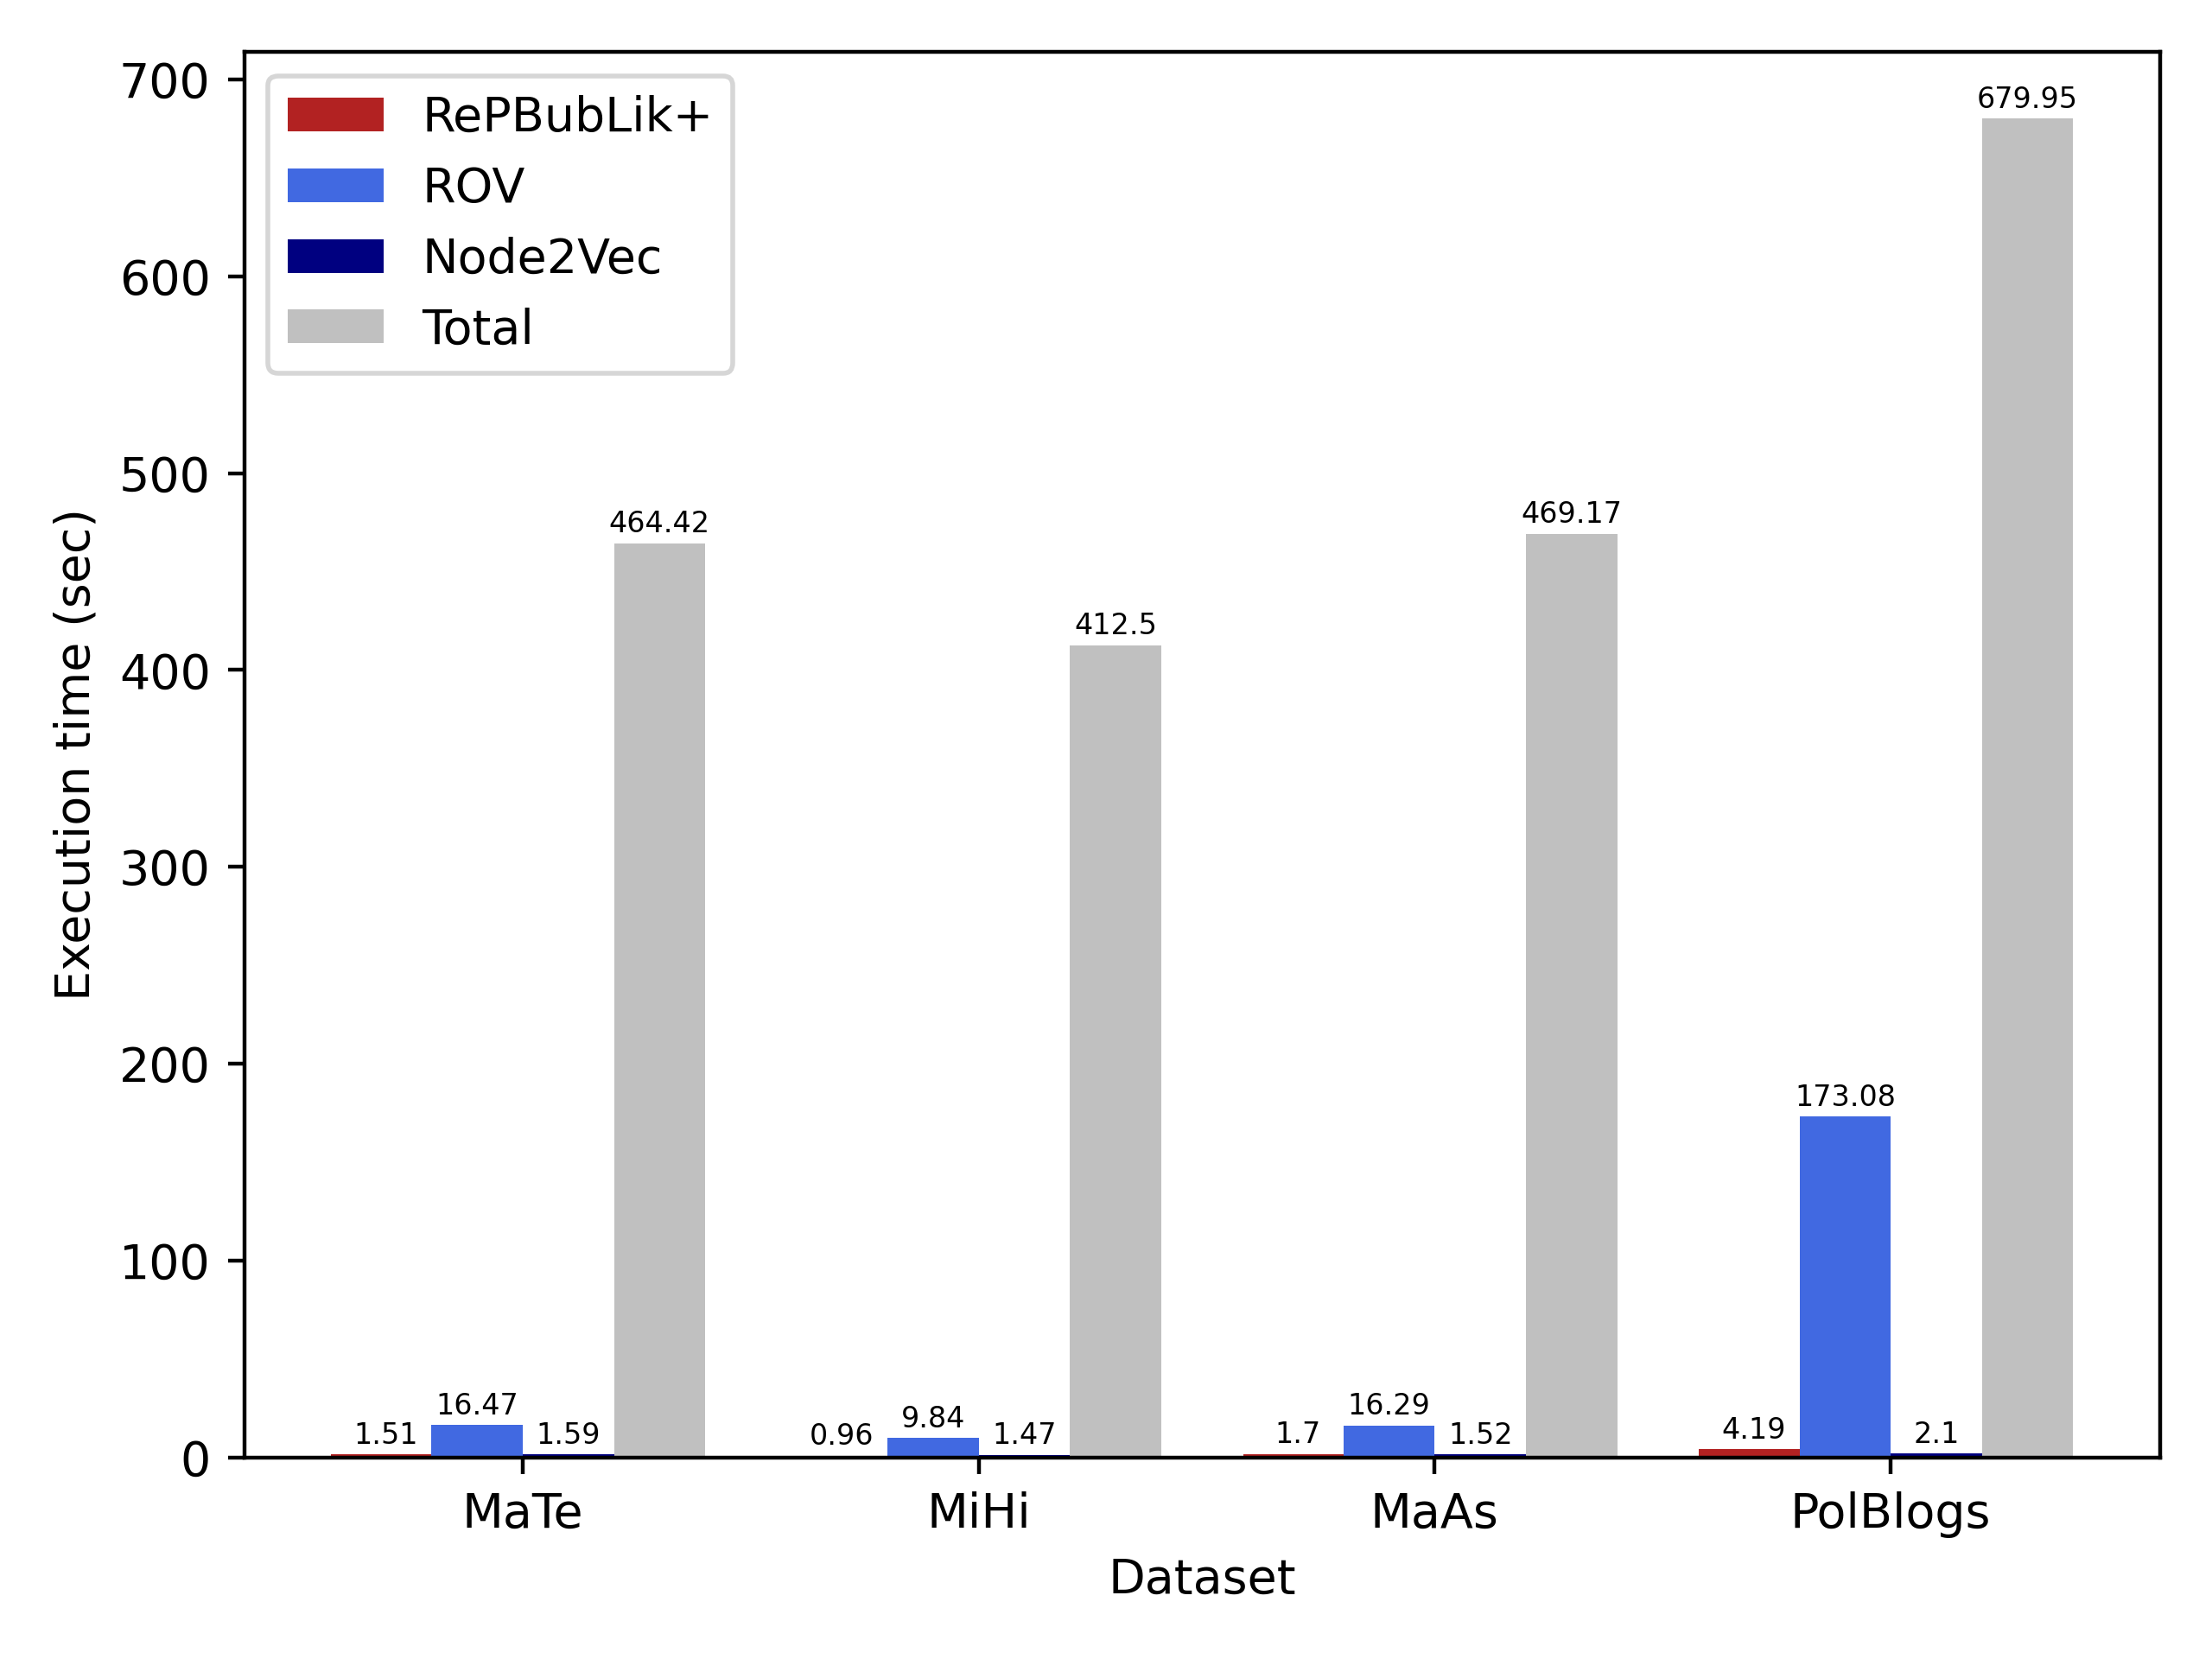
\includegraphics[width=\columnwidth]{5/ex_time_5.png}
    \caption{Parametro $t=5$}\label{fig:mate_e_5}
\end{subfigure}
\begin{subfigure}[h]{0.55\columnwidth}
    \centering
    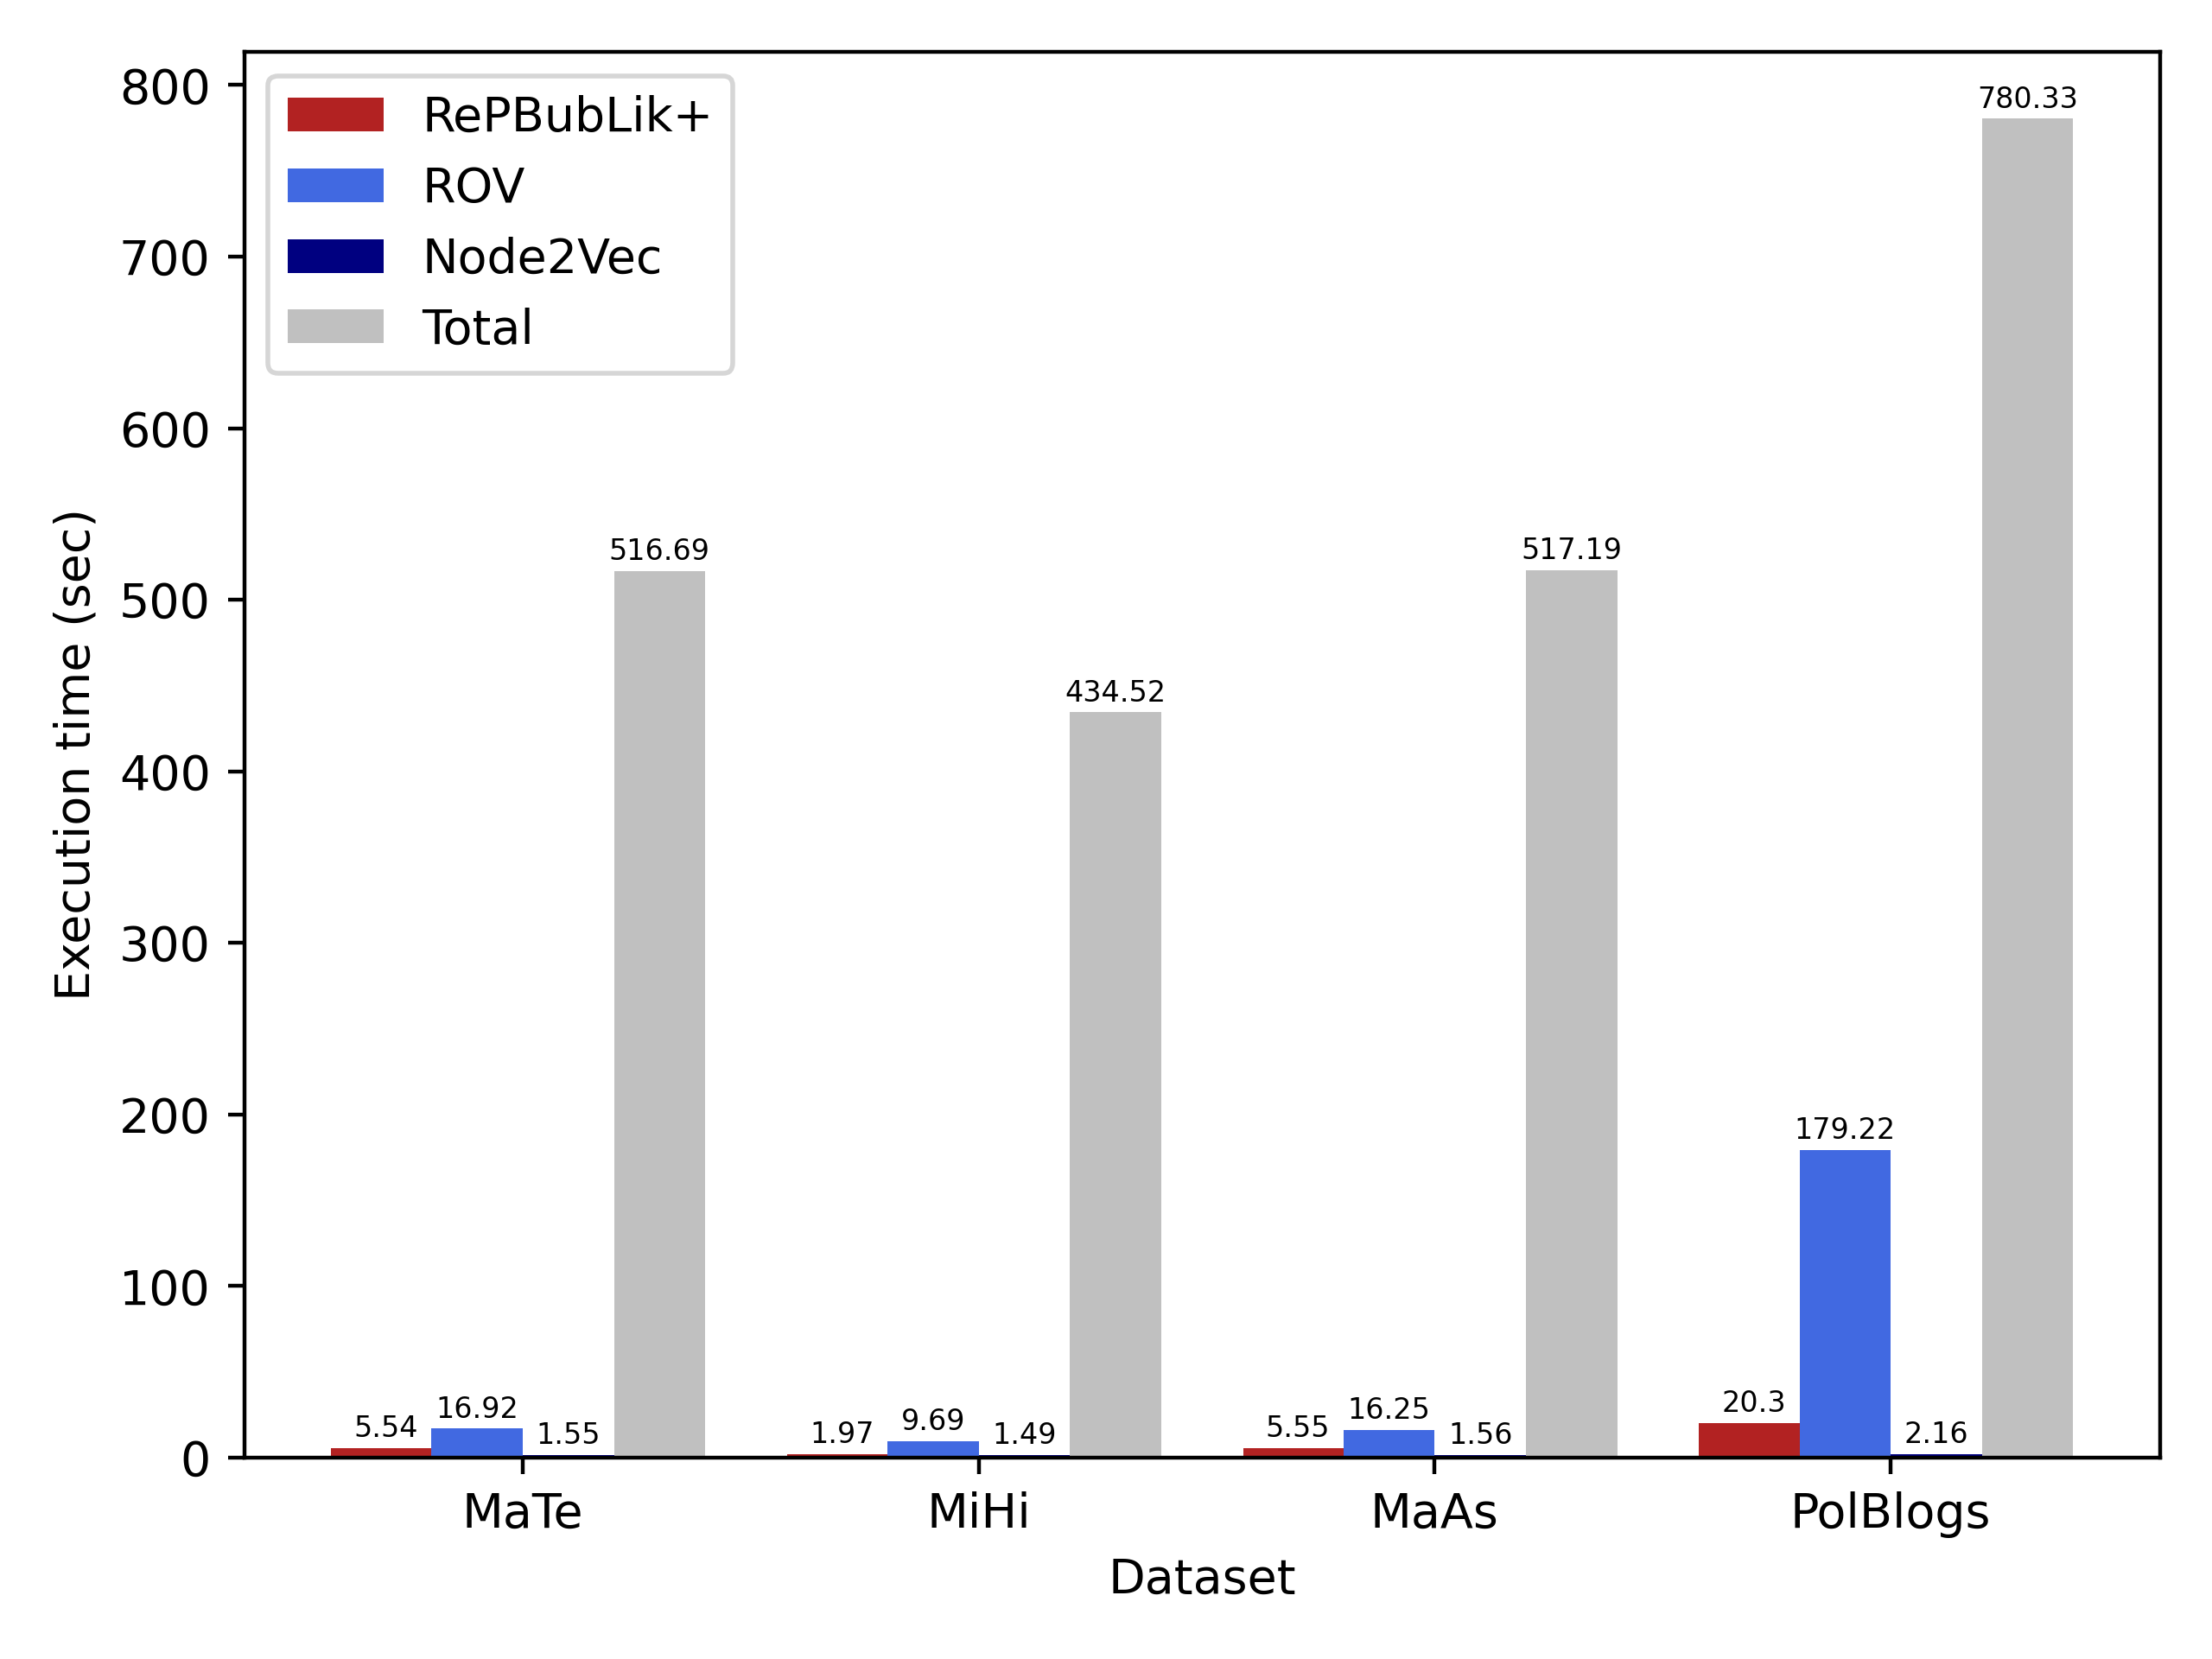
\includegraphics[width=\columnwidth]{10/ex_time_10.png}
    \caption{Parametro $t=10$}\label{fig:mihi_e_10}
\end{subfigure}
   
\end{figure}
\begin{figure}
\ContinuedFloat
\centering
\begin{subfigure}[h]{0.55\columnwidth}
    \centering
    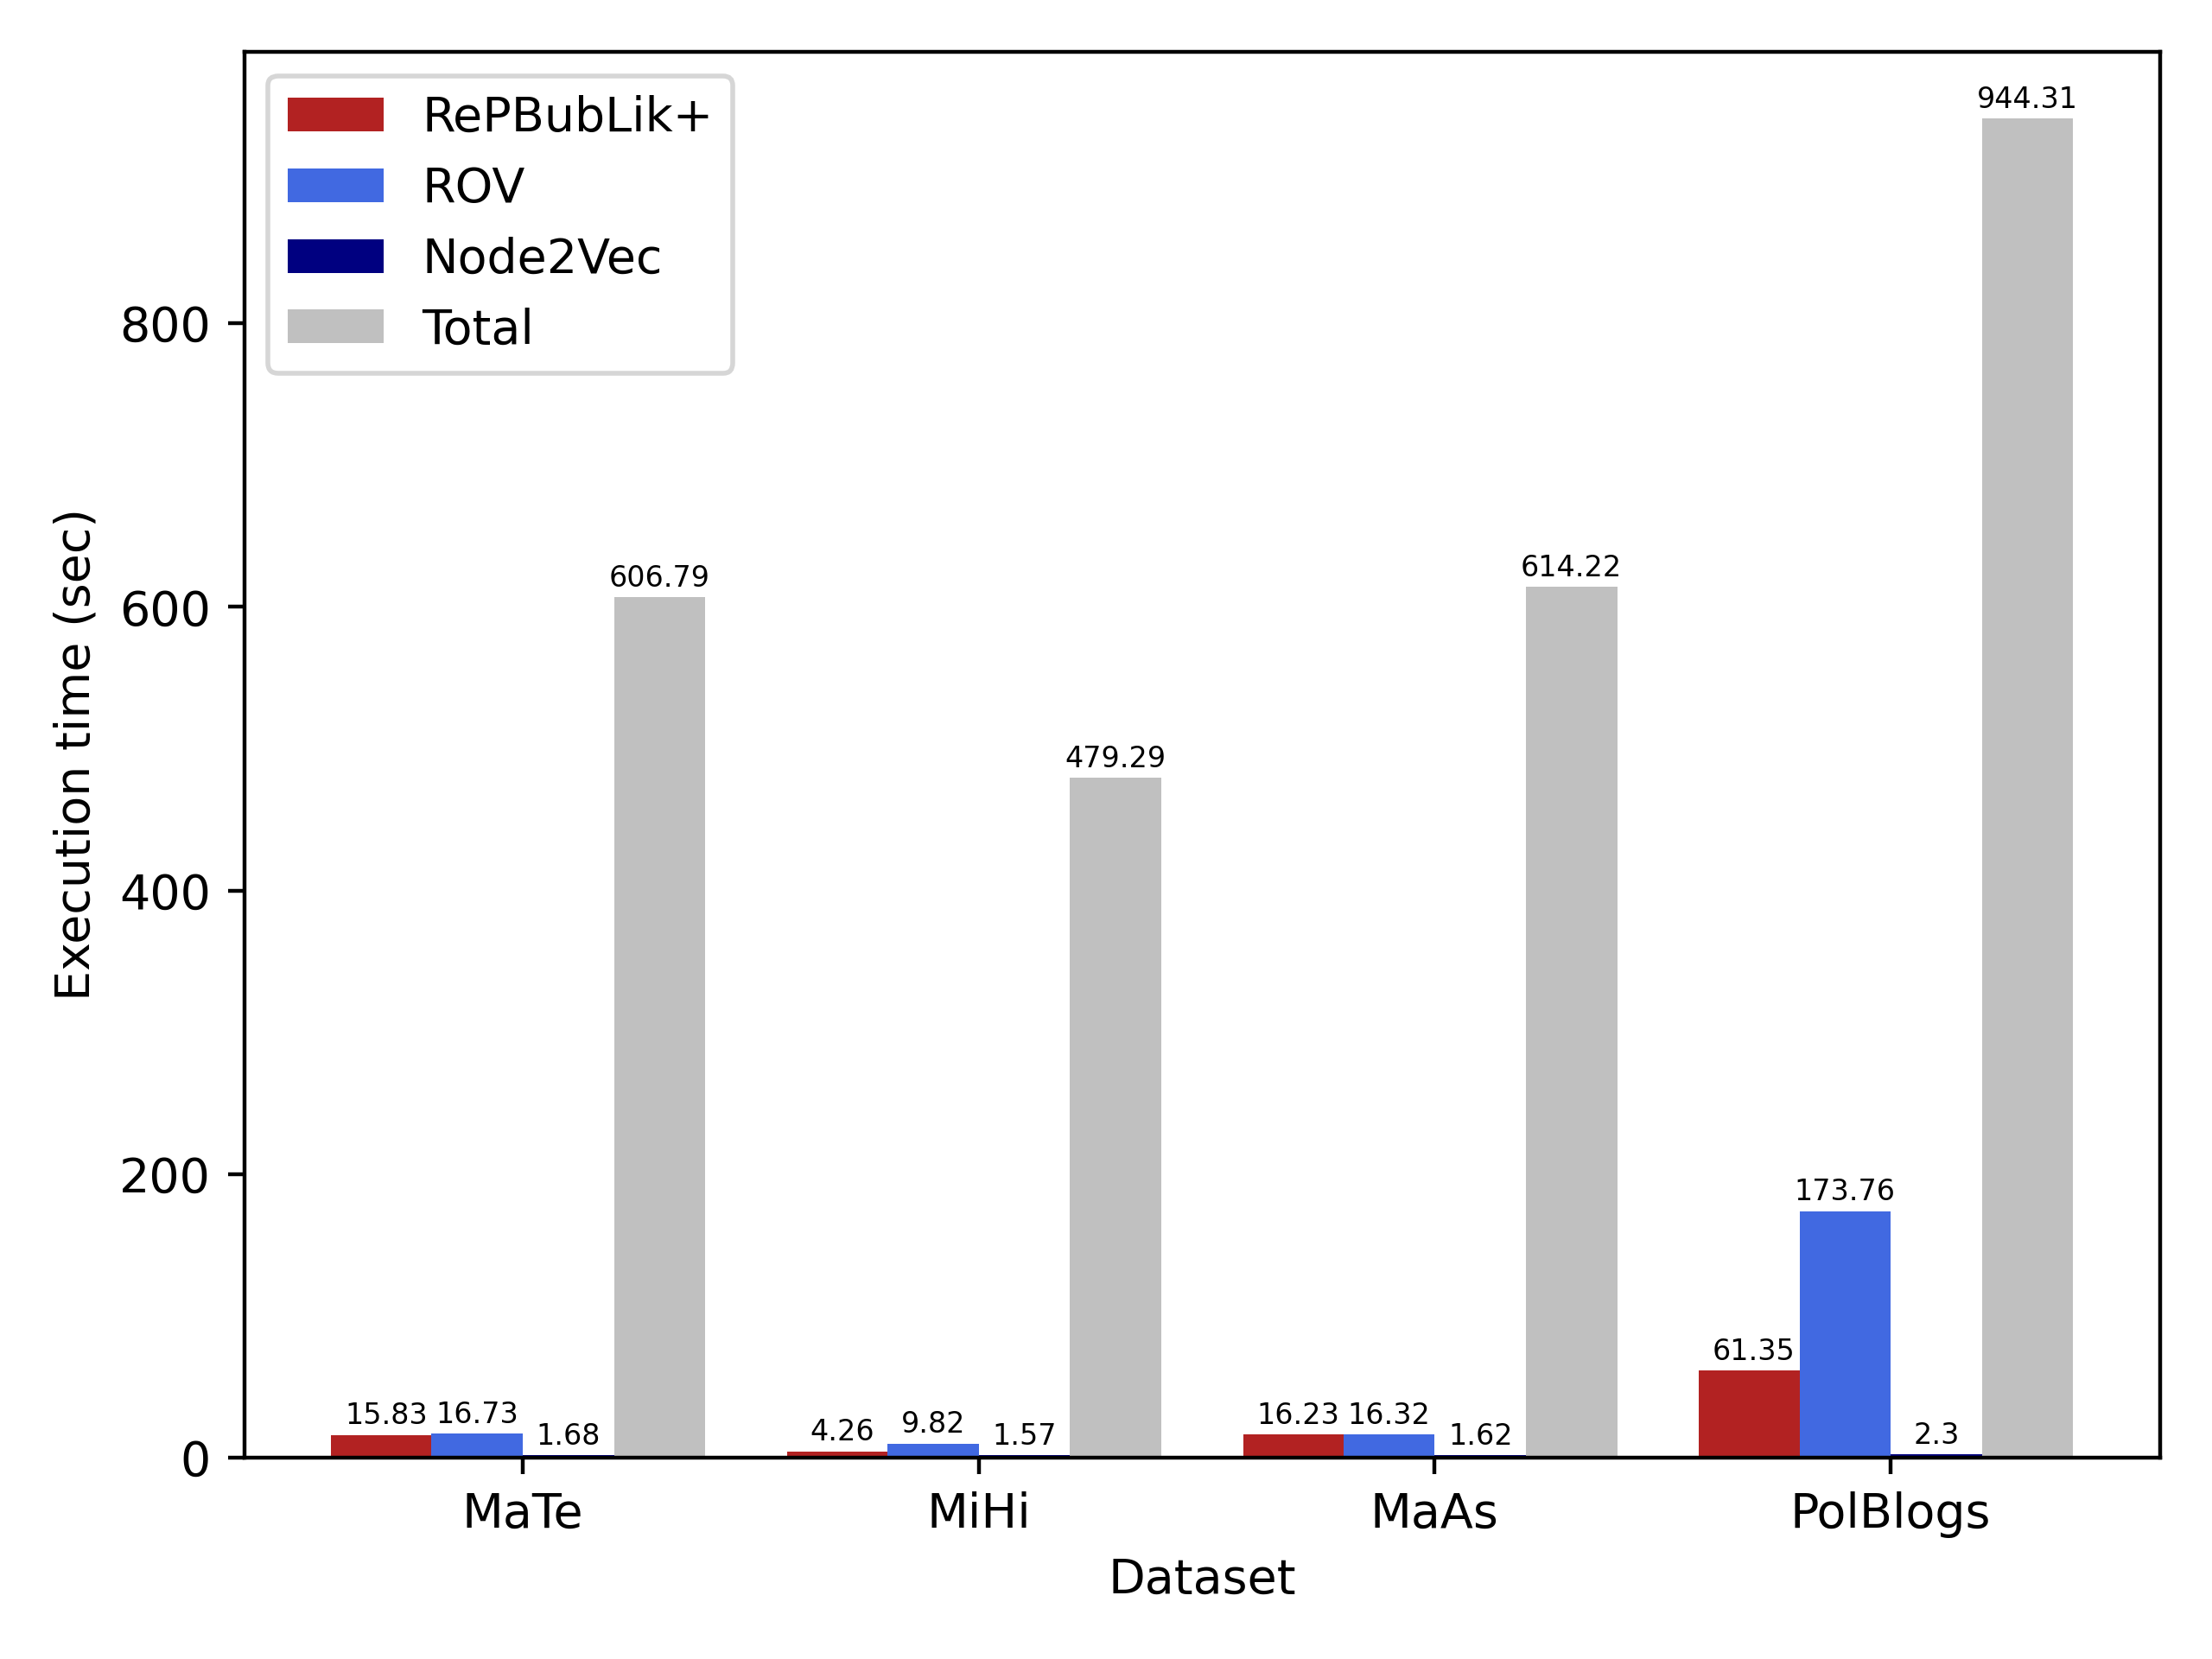
\includegraphics[width=\columnwidth]{15/ex_time_15.png}
    \caption{Parametro $t=15$}\label{fig:maas_e_15}
\end{subfigure}
\caption{Grafici dei tempi d'esecuzione}
\end{figure}
\newpage
Analizzando i grafici dei tempi di esecuzione, si possono trarre le seguenti conclusioni:
\begin{enumerate}
    \item Il tempo impiegato da ciascuna procedura aumenta in relazione alle dimensioni del grafo su cui è applicata.
    \item Node2Vec risulta essere il migliore in termini di tempo d'esecuzione, per ogni grafo e per ogni valore di $t$.
    \item Per ciascun grafo, l'esecuzione di ROV impiega all'incirca lo stesso tempo, indipendentemente dal valore di $t$. 
            Questo è dato dal fatto che ROV utilizza delle metriche differenti dagli altri algoritmi proposti.
    \item RePBubLik+ ha tempistiche intermedie tra quelle di ROV e Node2Vec.
\end{enumerate}
\subsection{Guadagno $\Delta(G,\Sigma)$}
La seconda metrica che viene anlizzata è il il guadagno $\Delta(G,\Sigma)$ (\ref{REP:gain}) in relazione al numero 
degli archi aggiunti al grafo $G$. Lo studio di questa misura è interessante, in quanto permette di valutare il cambiamento medio del Bubble Radius dei vertici parochial $P(G)$.
\\
Nella pagina successiva, i guadagni per ciascun grafo e per ciascun valore di $t$.
\begin{figure}[!h]
    \centering
\begin{subfigure}[h]{0.4\textwidth}
    \centering
    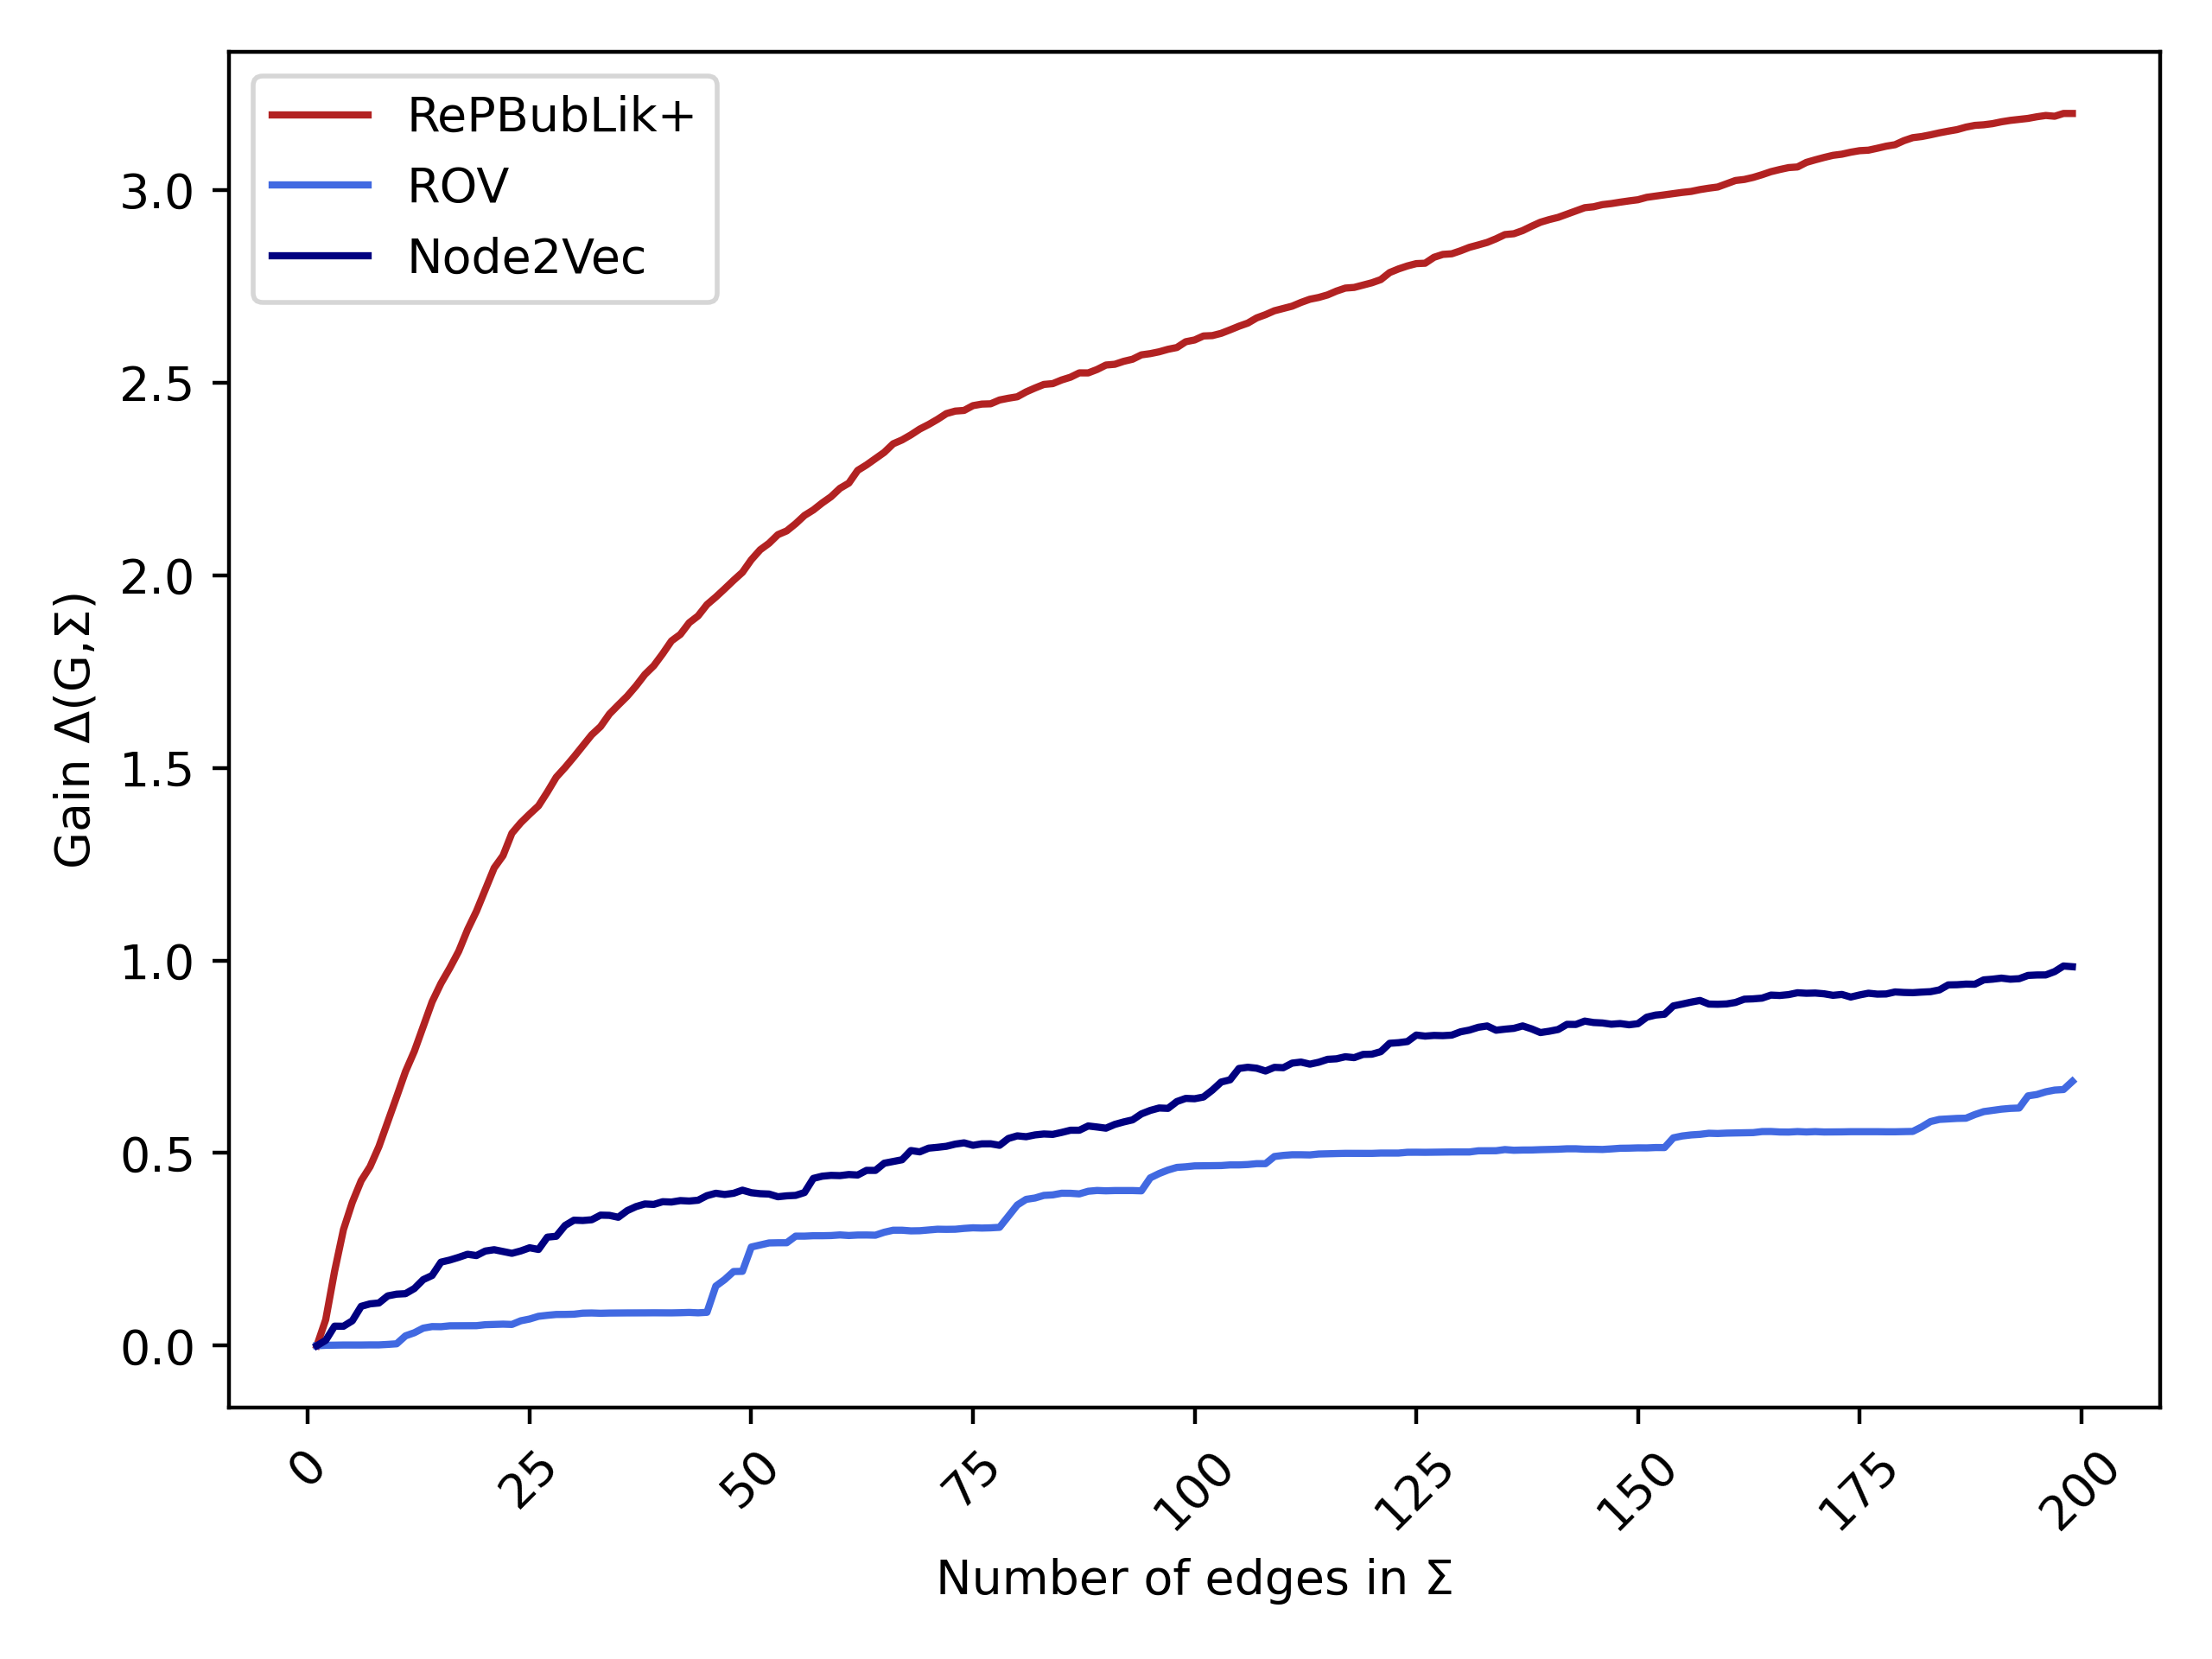
\includegraphics[width=\columnwidth]{5/math_tech_gain_5.png}
    \caption{\emph{MaTe} plot}\label{fig:mate_g_5}
\end{subfigure}
\hspace{0.1\columnwidth}
\begin{subfigure}[h]{0.4\textwidth}
    \centering
    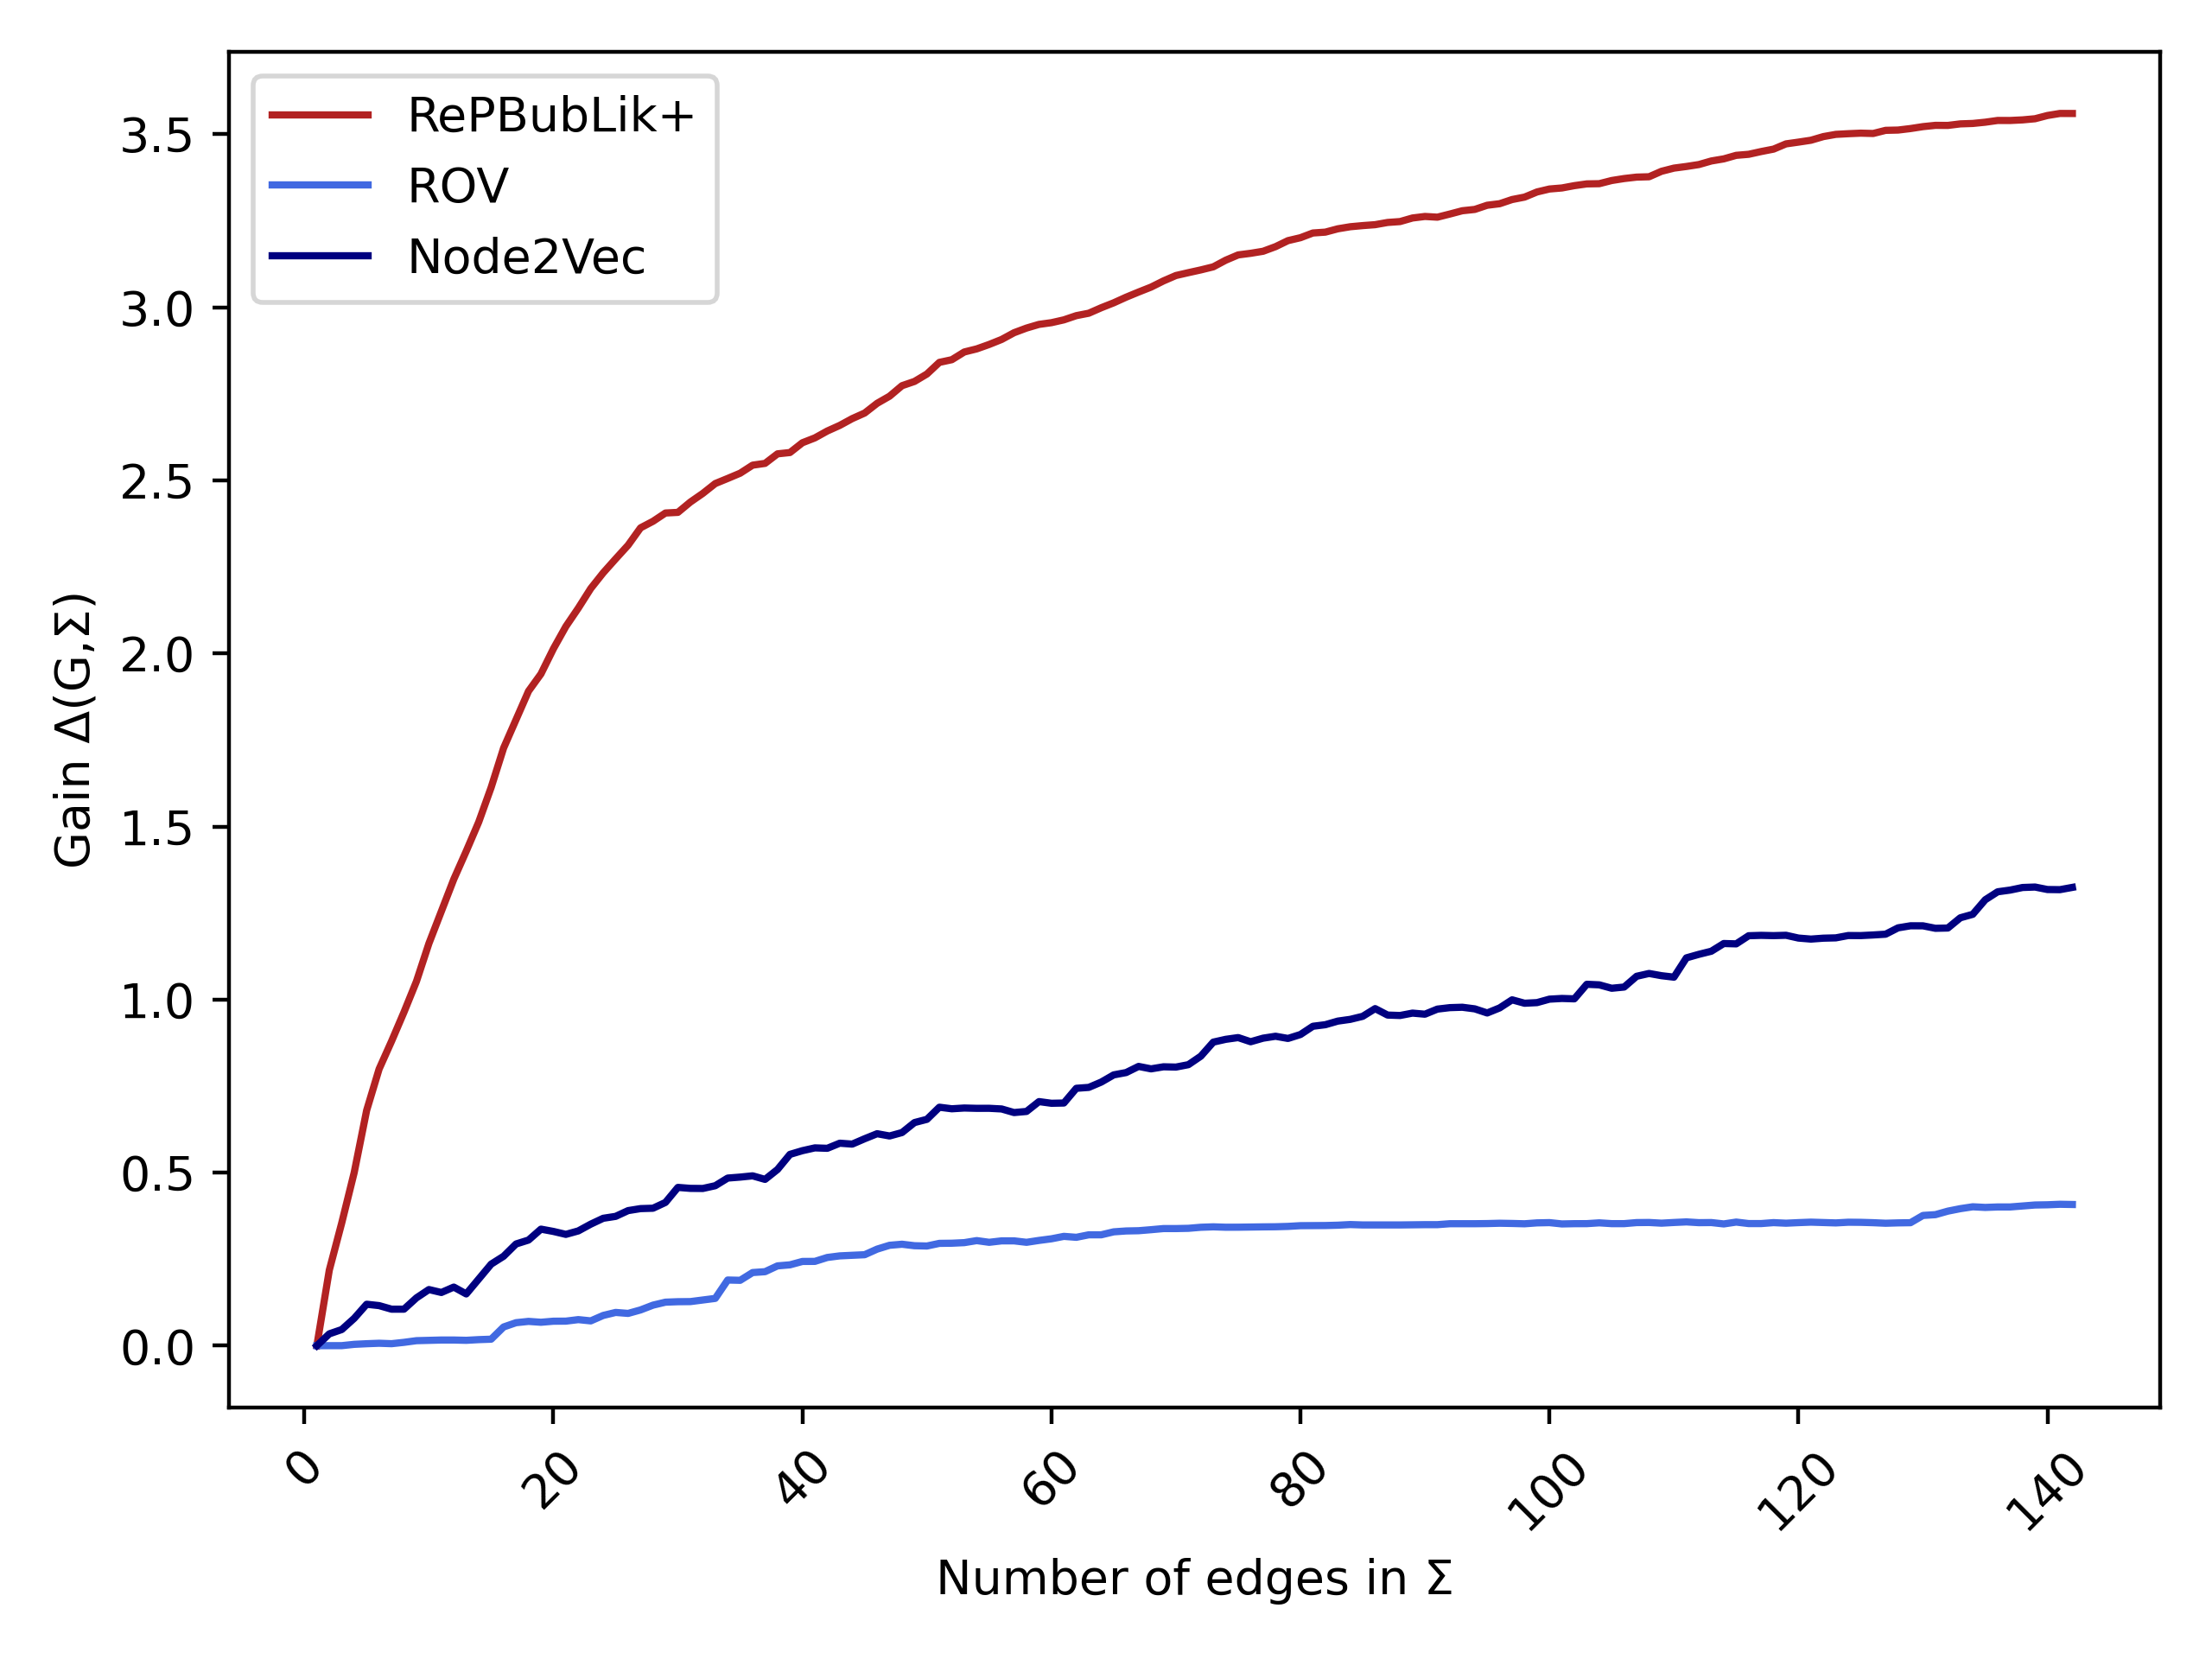
\includegraphics[width=\columnwidth]{5/tech_mil_gain_5.png}
    \caption{\emph{MiHi} plot}\label{fig:mihi_g_5}
\end{subfigure}
\end{figure}
\begin{figure}
    \ContinuedFloat
    \centering
\begin{subfigure}[h]{0.4\textwidth}
    \centering
    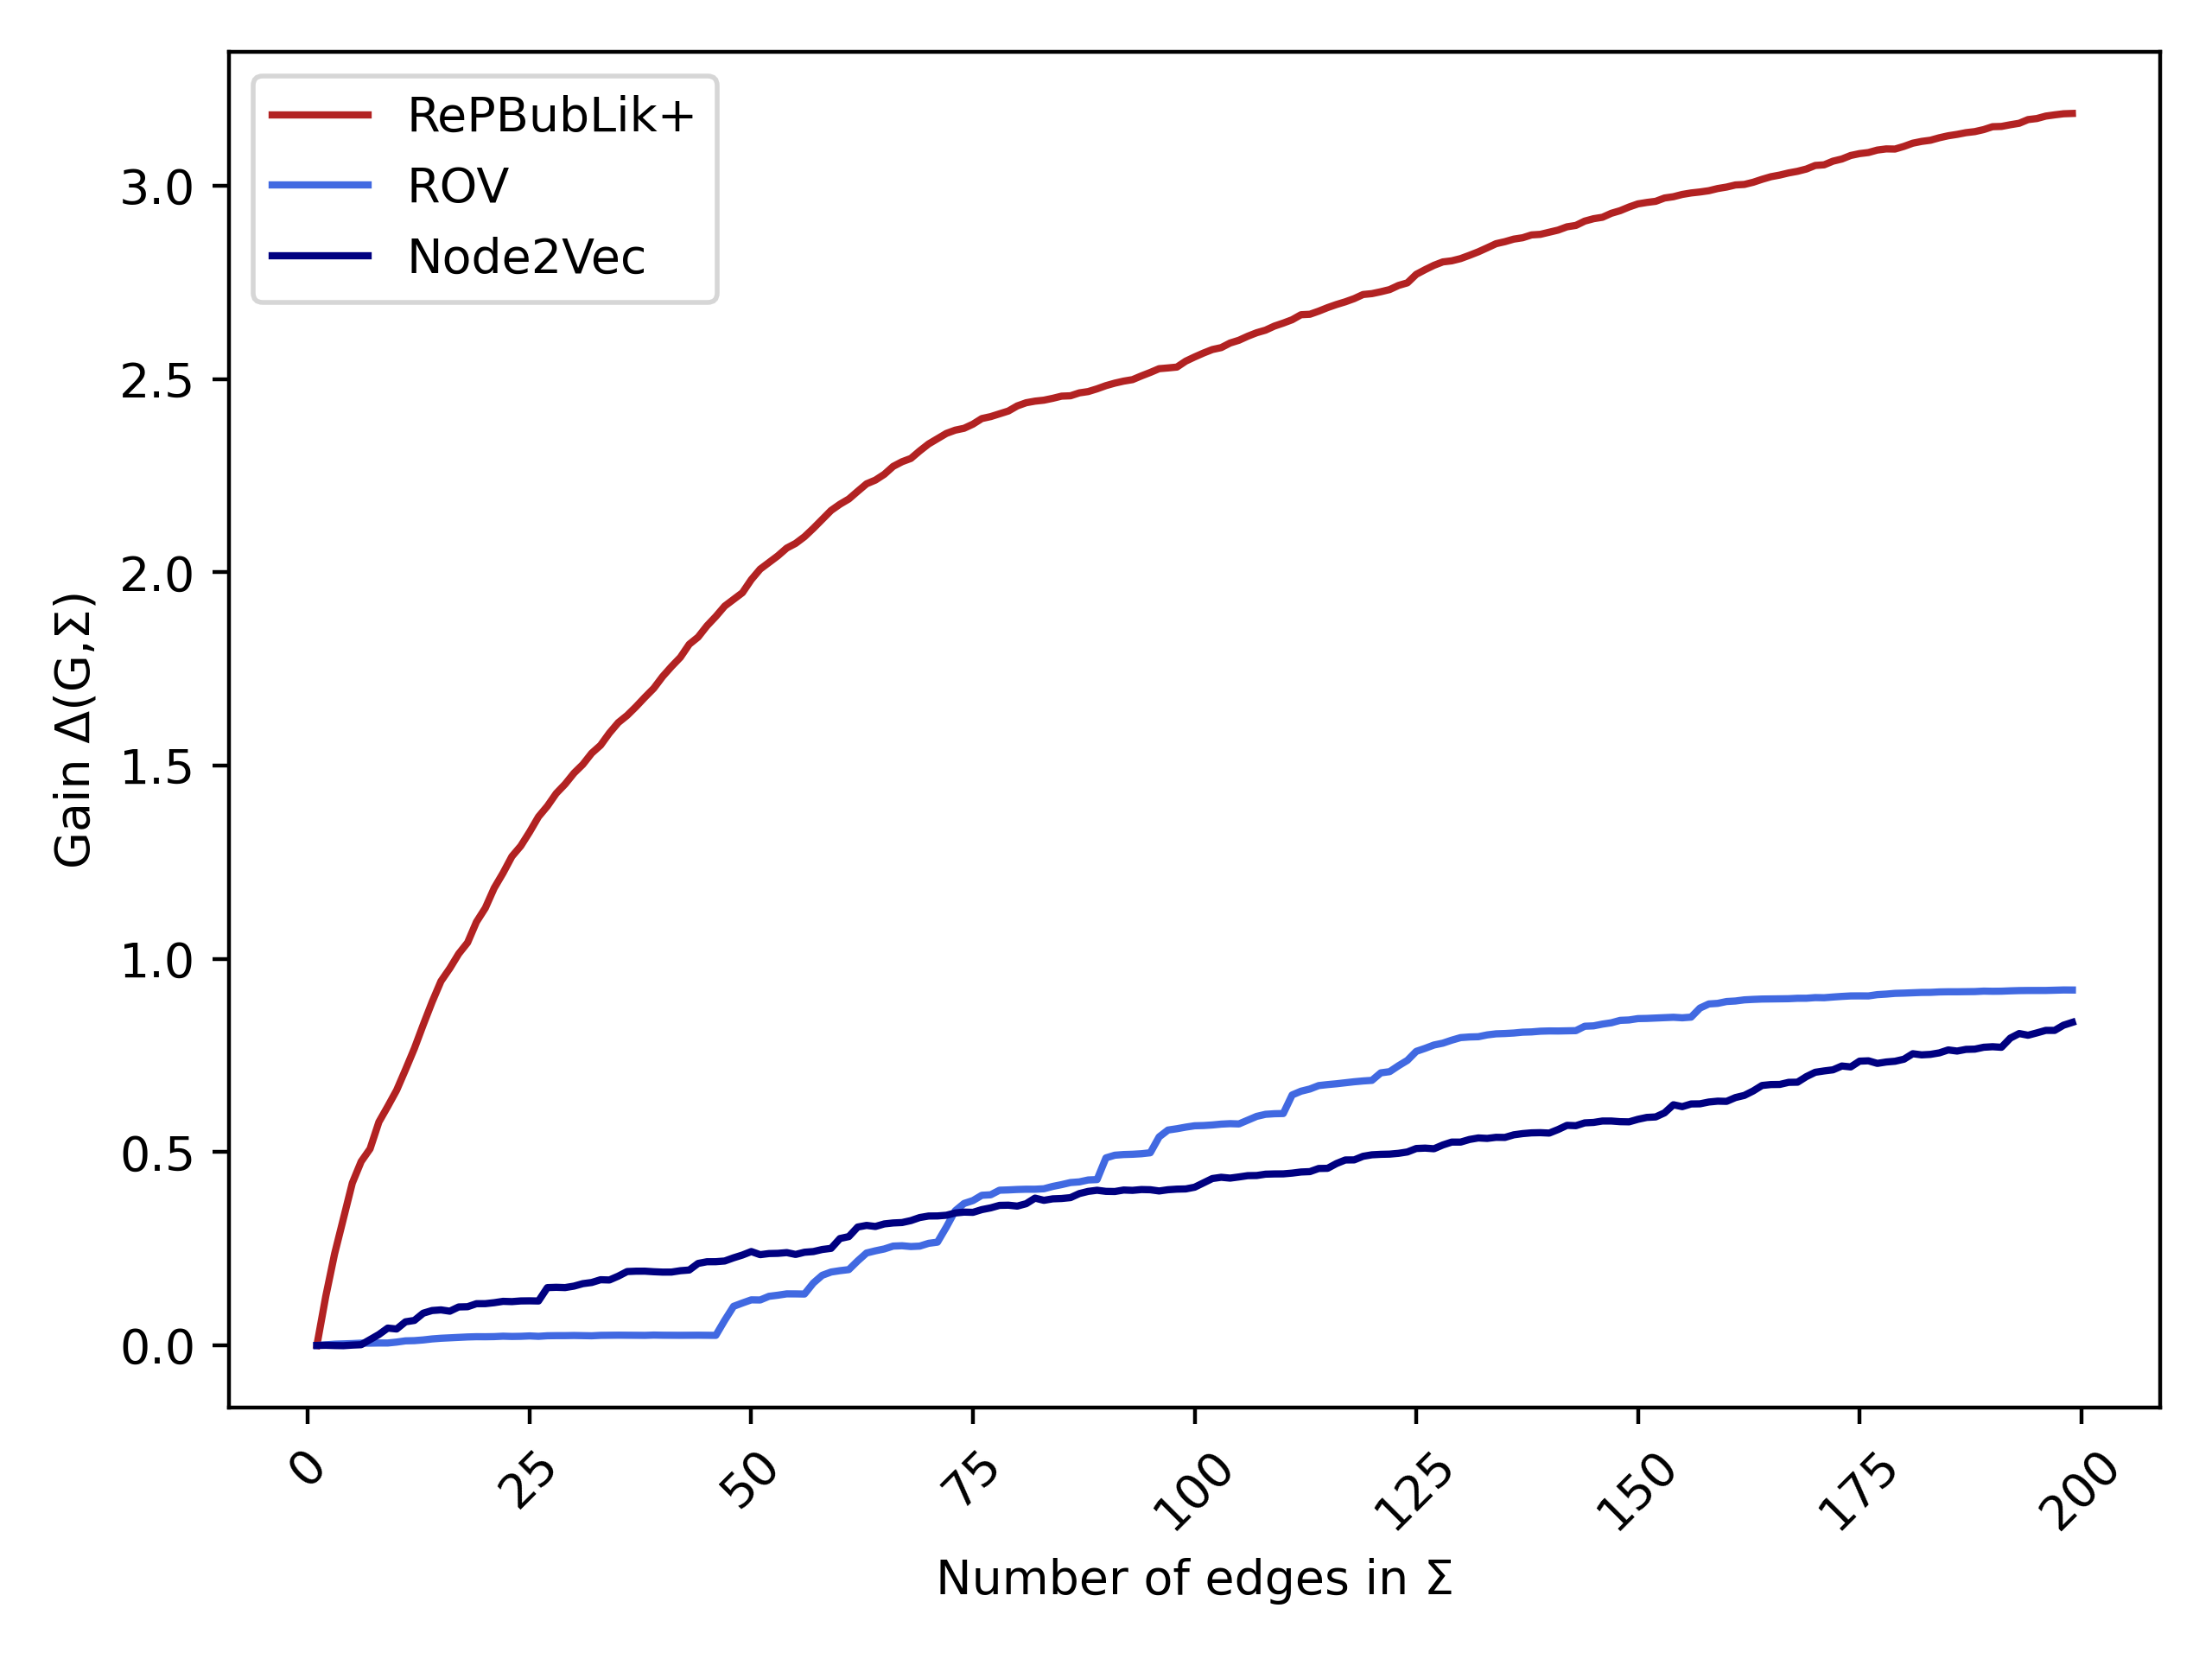
\includegraphics[width=\columnwidth]{5/math_ast_gain_5.png}
    \caption{\emph{MaA}s plot}\label{fig:maas_g_5}
\end{subfigure}
\hspace{0.1\columnwidth}
\begin{subfigure}[h]{0.4\textwidth}
    \centering
    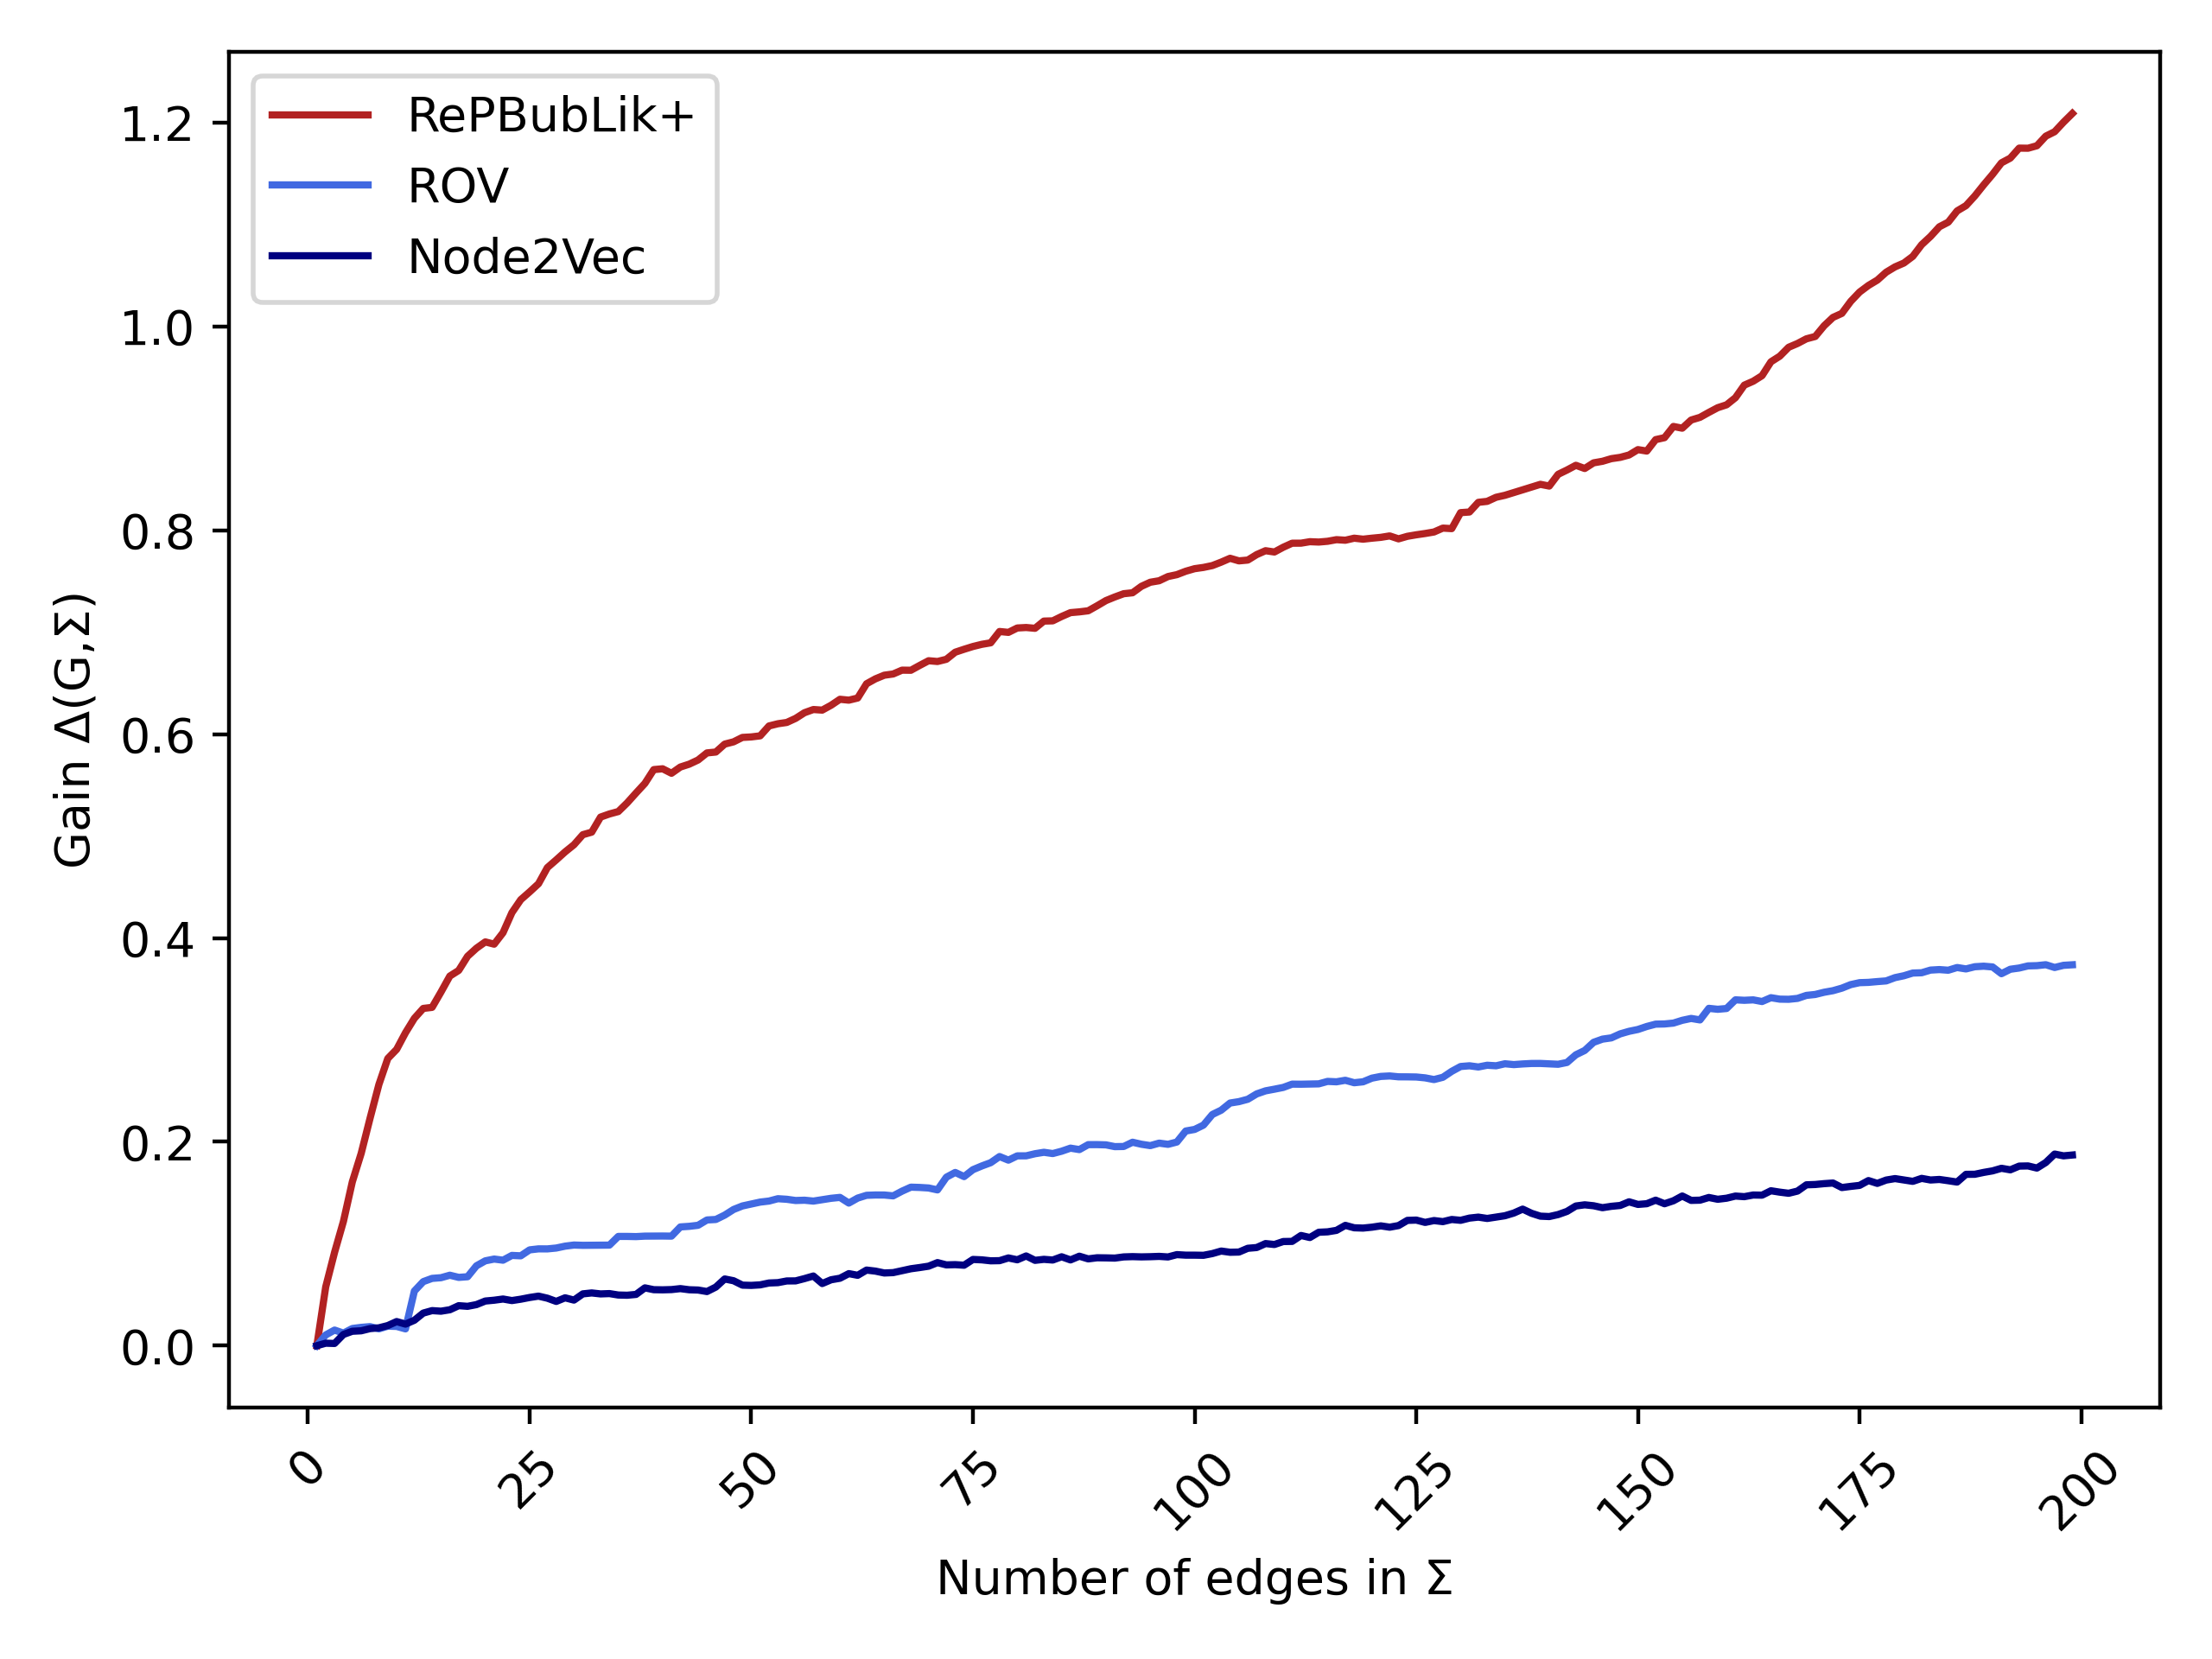
\includegraphics[width=\columnwidth]{5/polblogs_gain_5.png}
    \caption{\emph{PolBlogs} plot}\label{fig:polblogs_g_5}
\end{subfigure}
\caption{Grafici $\Delta(G,\Sigma)$ per $t=5$}
\end{figure}
\begin{figure}[!h]
    \centering
\begin{subfigure}[b]{0.4\textwidth}
    \centering
    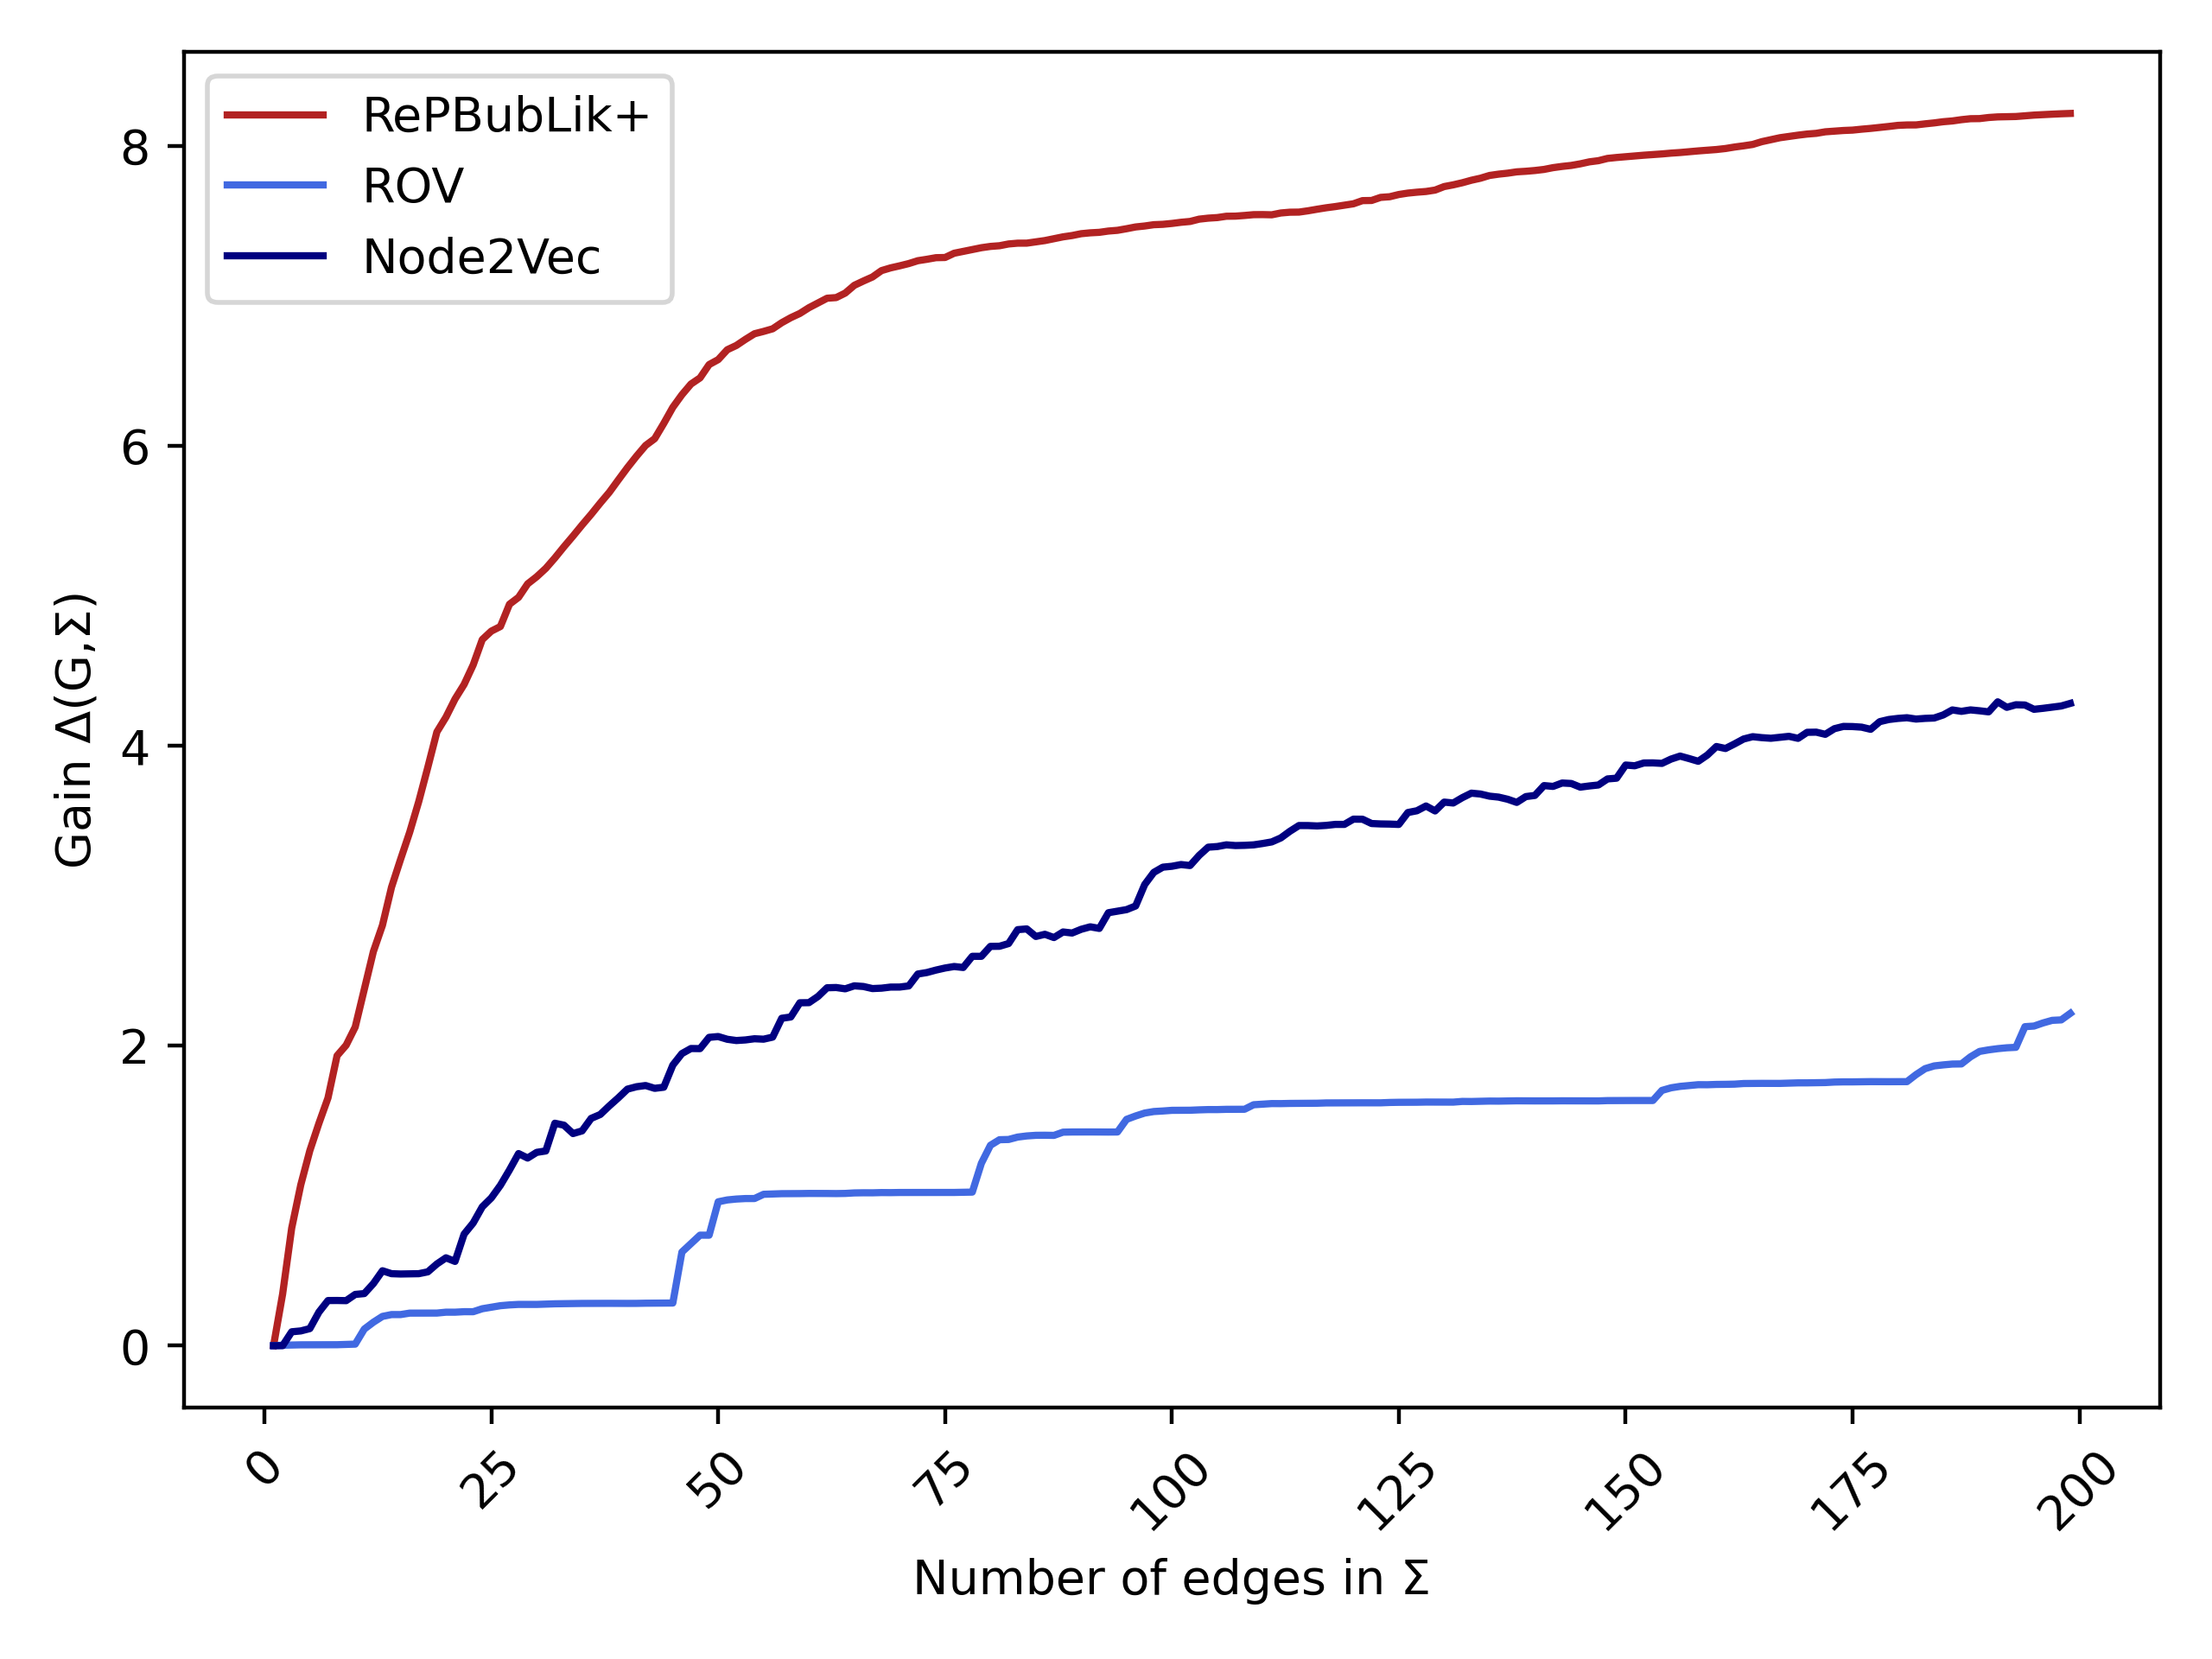
\includegraphics[width=\columnwidth]{10/math_tech_gain_10.png}
    \caption{\emph{MaTe} plot}\label{fig:mate_g_10}
\end{subfigure}
\hspace{0.1\columnwidth}
\begin{subfigure}[b]{0.4\textwidth}
    \centering
    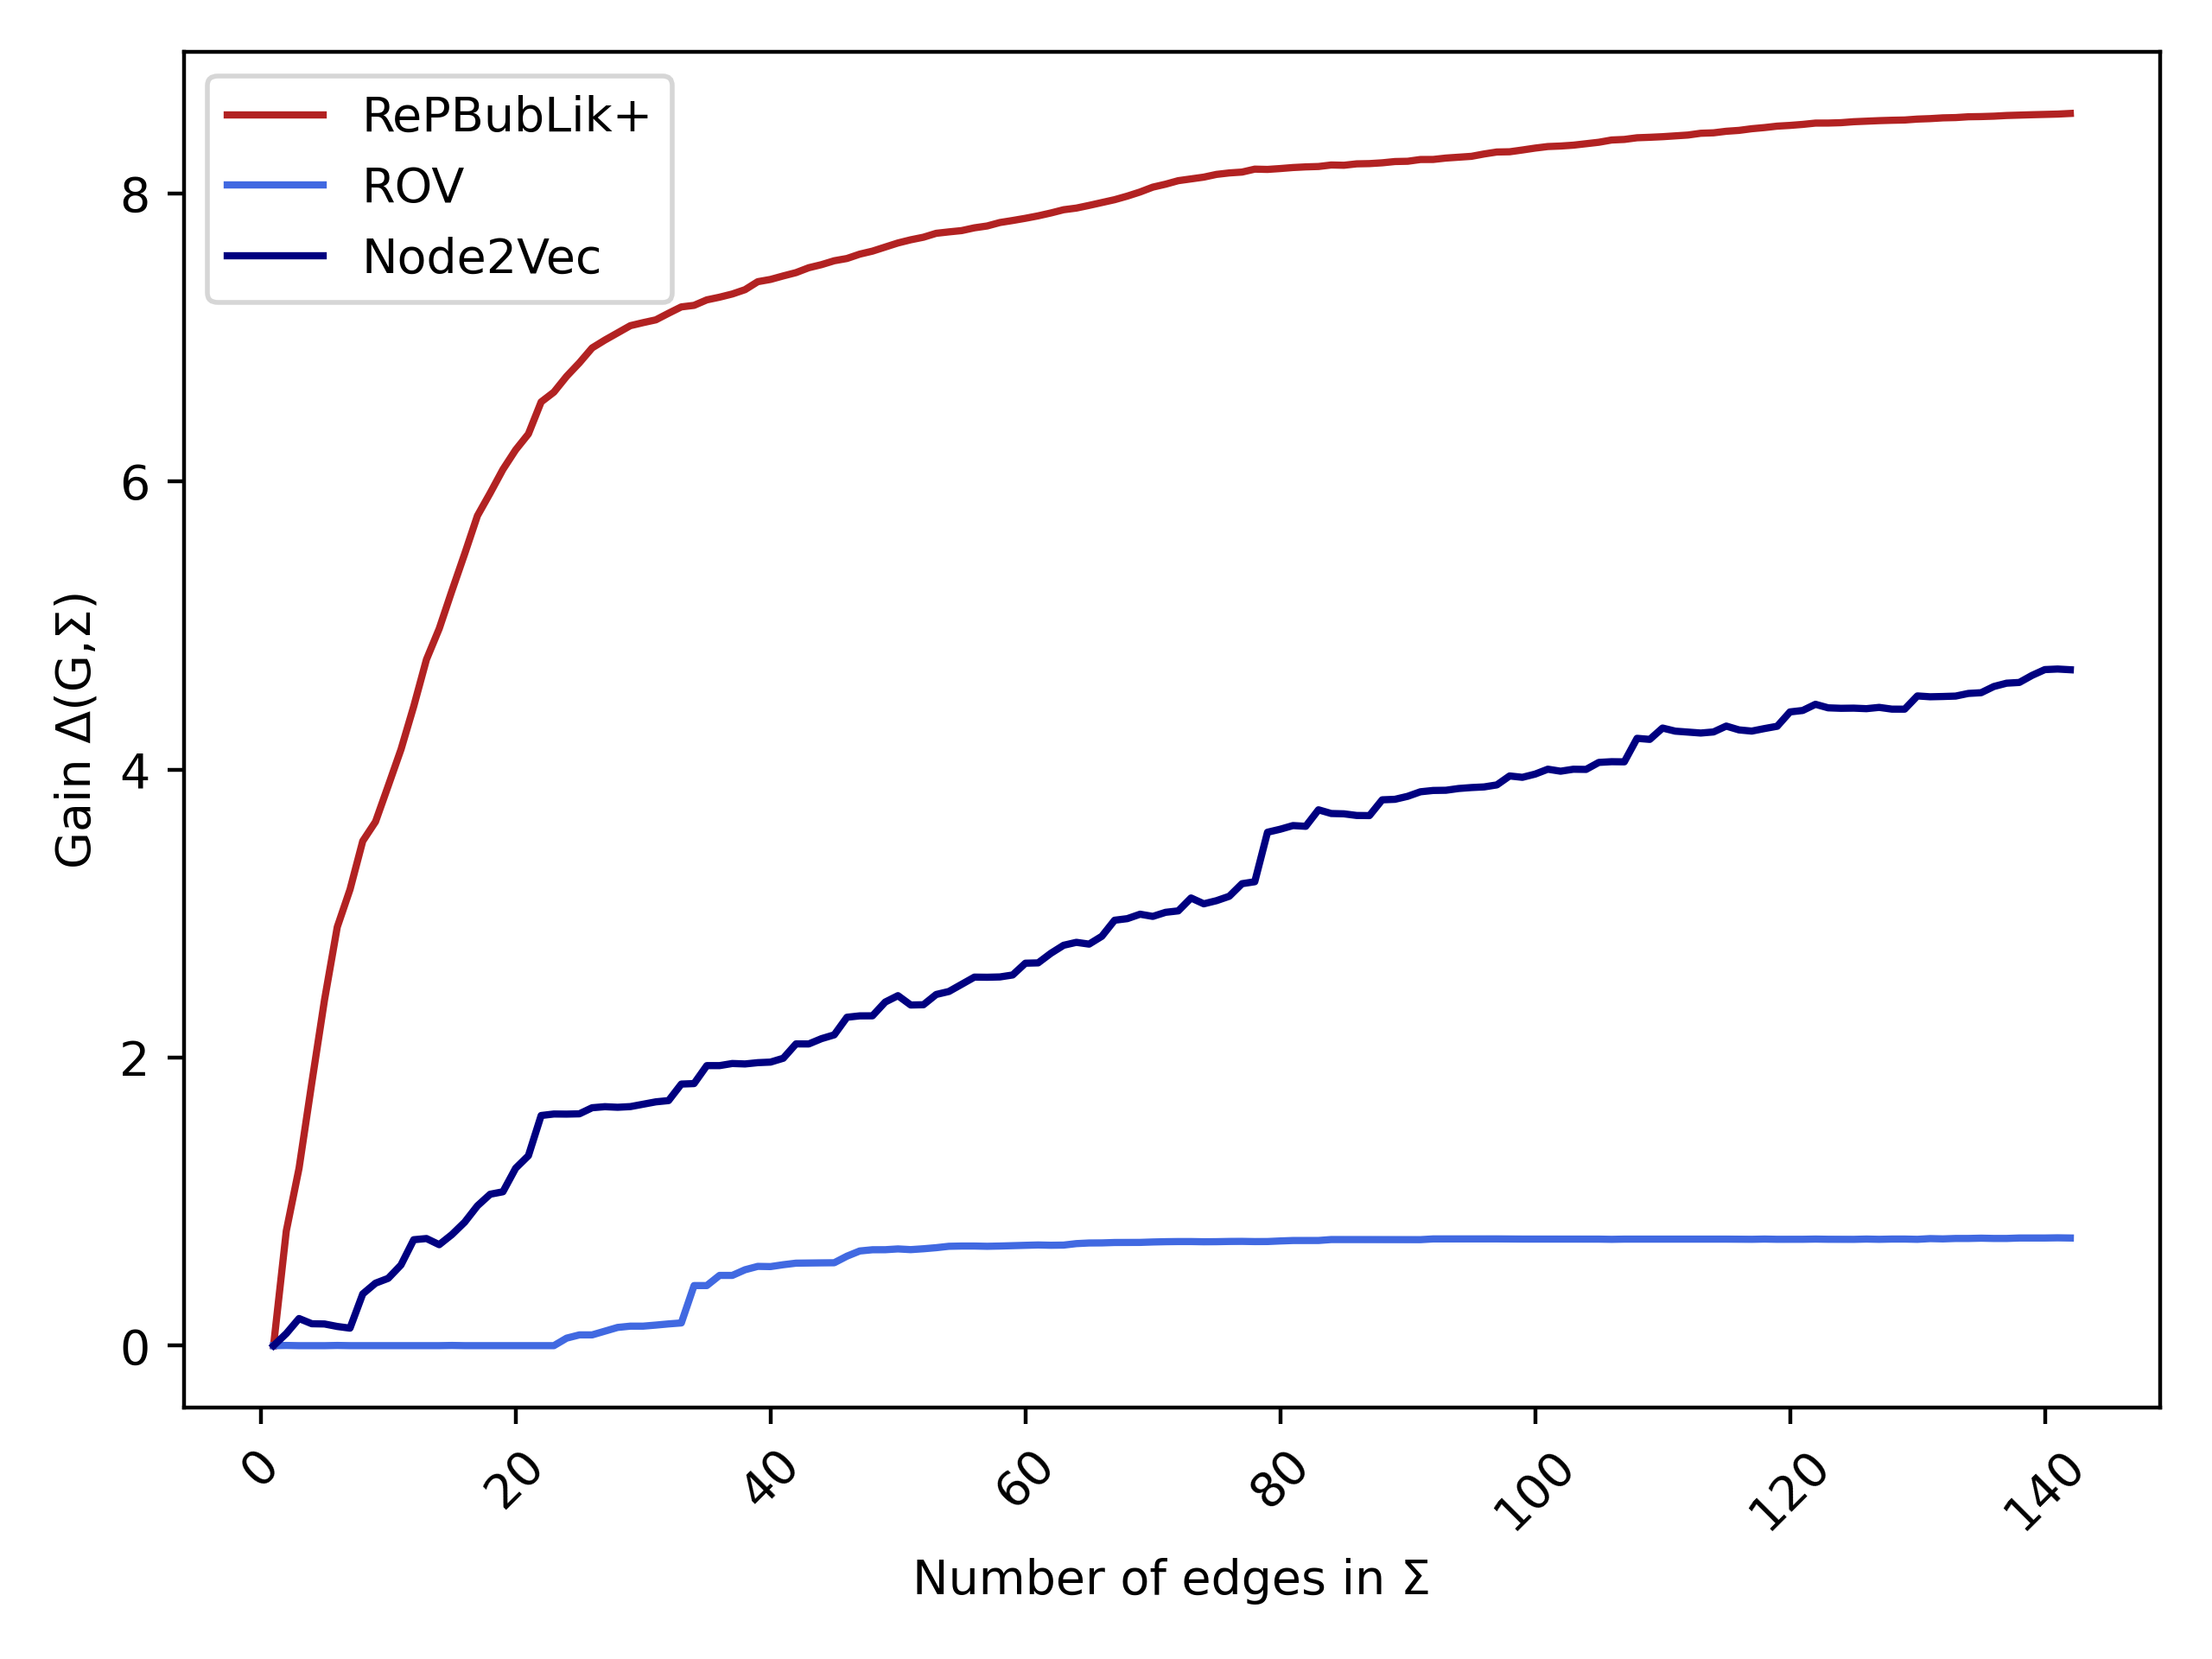
\includegraphics[width=\columnwidth]{10/tech_mil_gain_10.png}
    \caption{\emph{MiHi} plot}\label{fig:mihi_g_10}
\end{subfigure}

\begin{subfigure}[b]{0.4\textwidth}
    \centering
    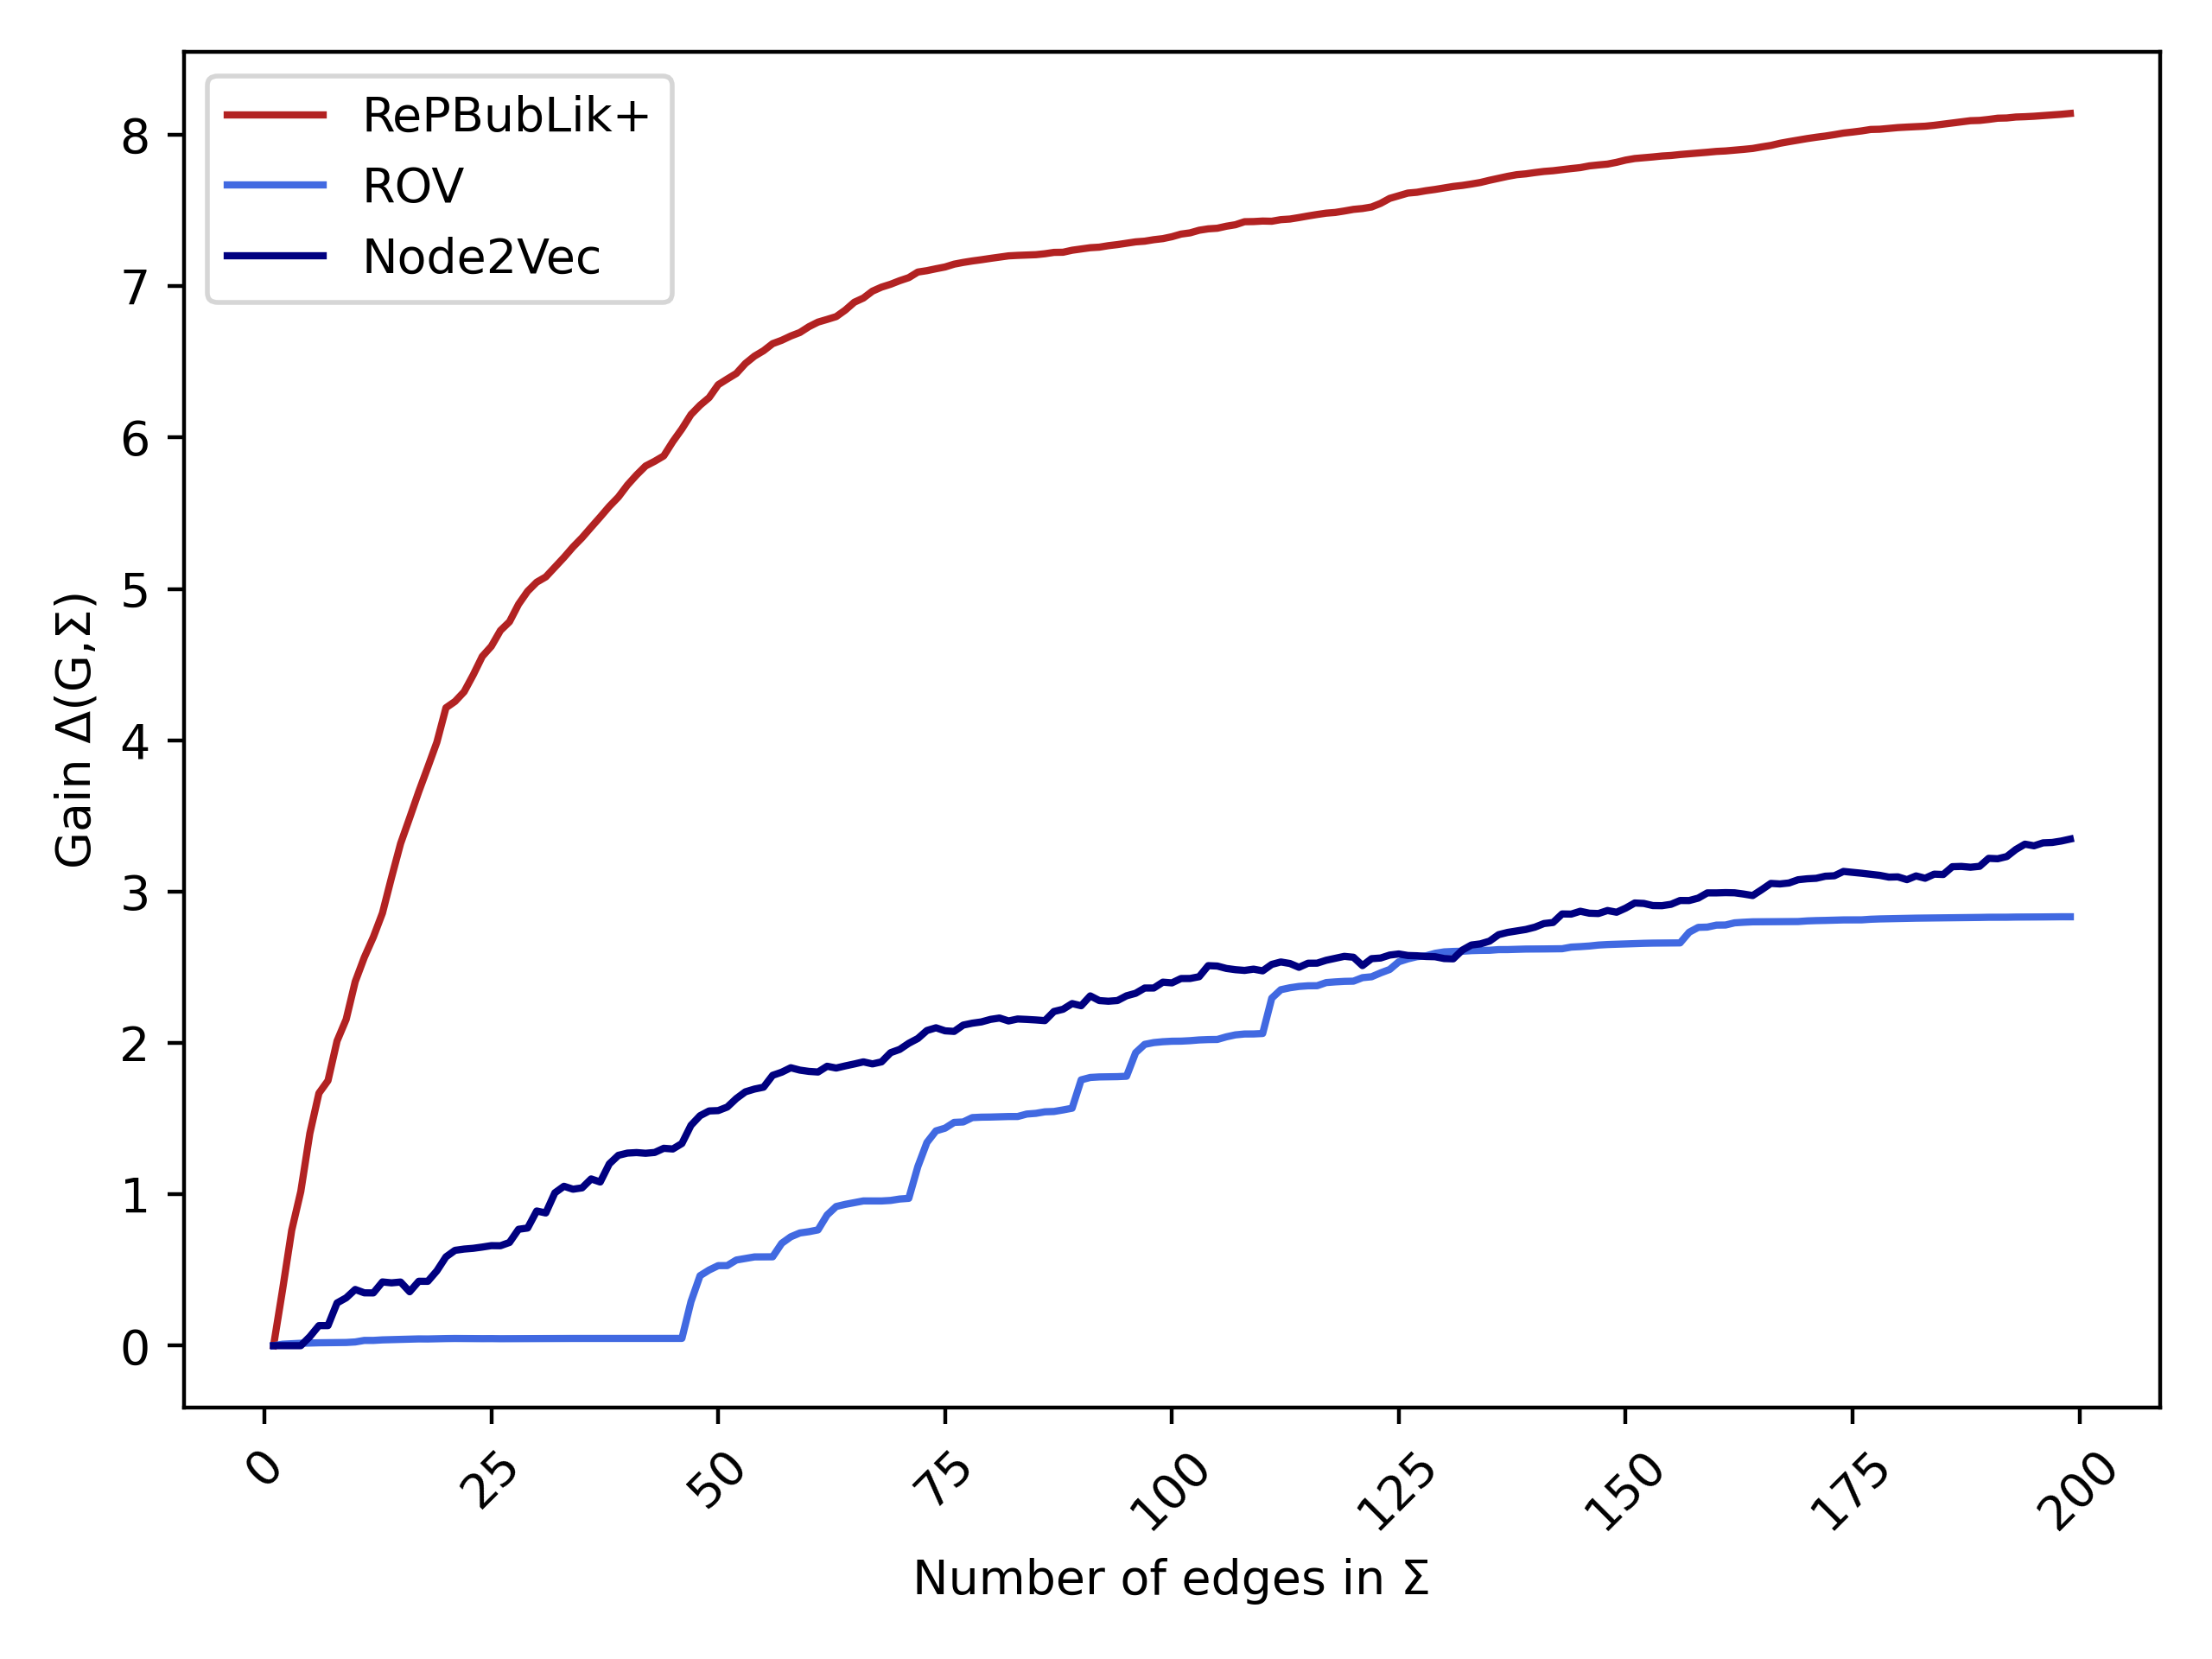
\includegraphics[width=\columnwidth]{10/math_ast_gain_10.png}
    \caption{\emph{MaA}s plot}\label{fig:maas_g_10}
\end{subfigure}
\hspace{0.1\columnwidth}
\begin{subfigure}[b]{0.4\textwidth}
    \centering
    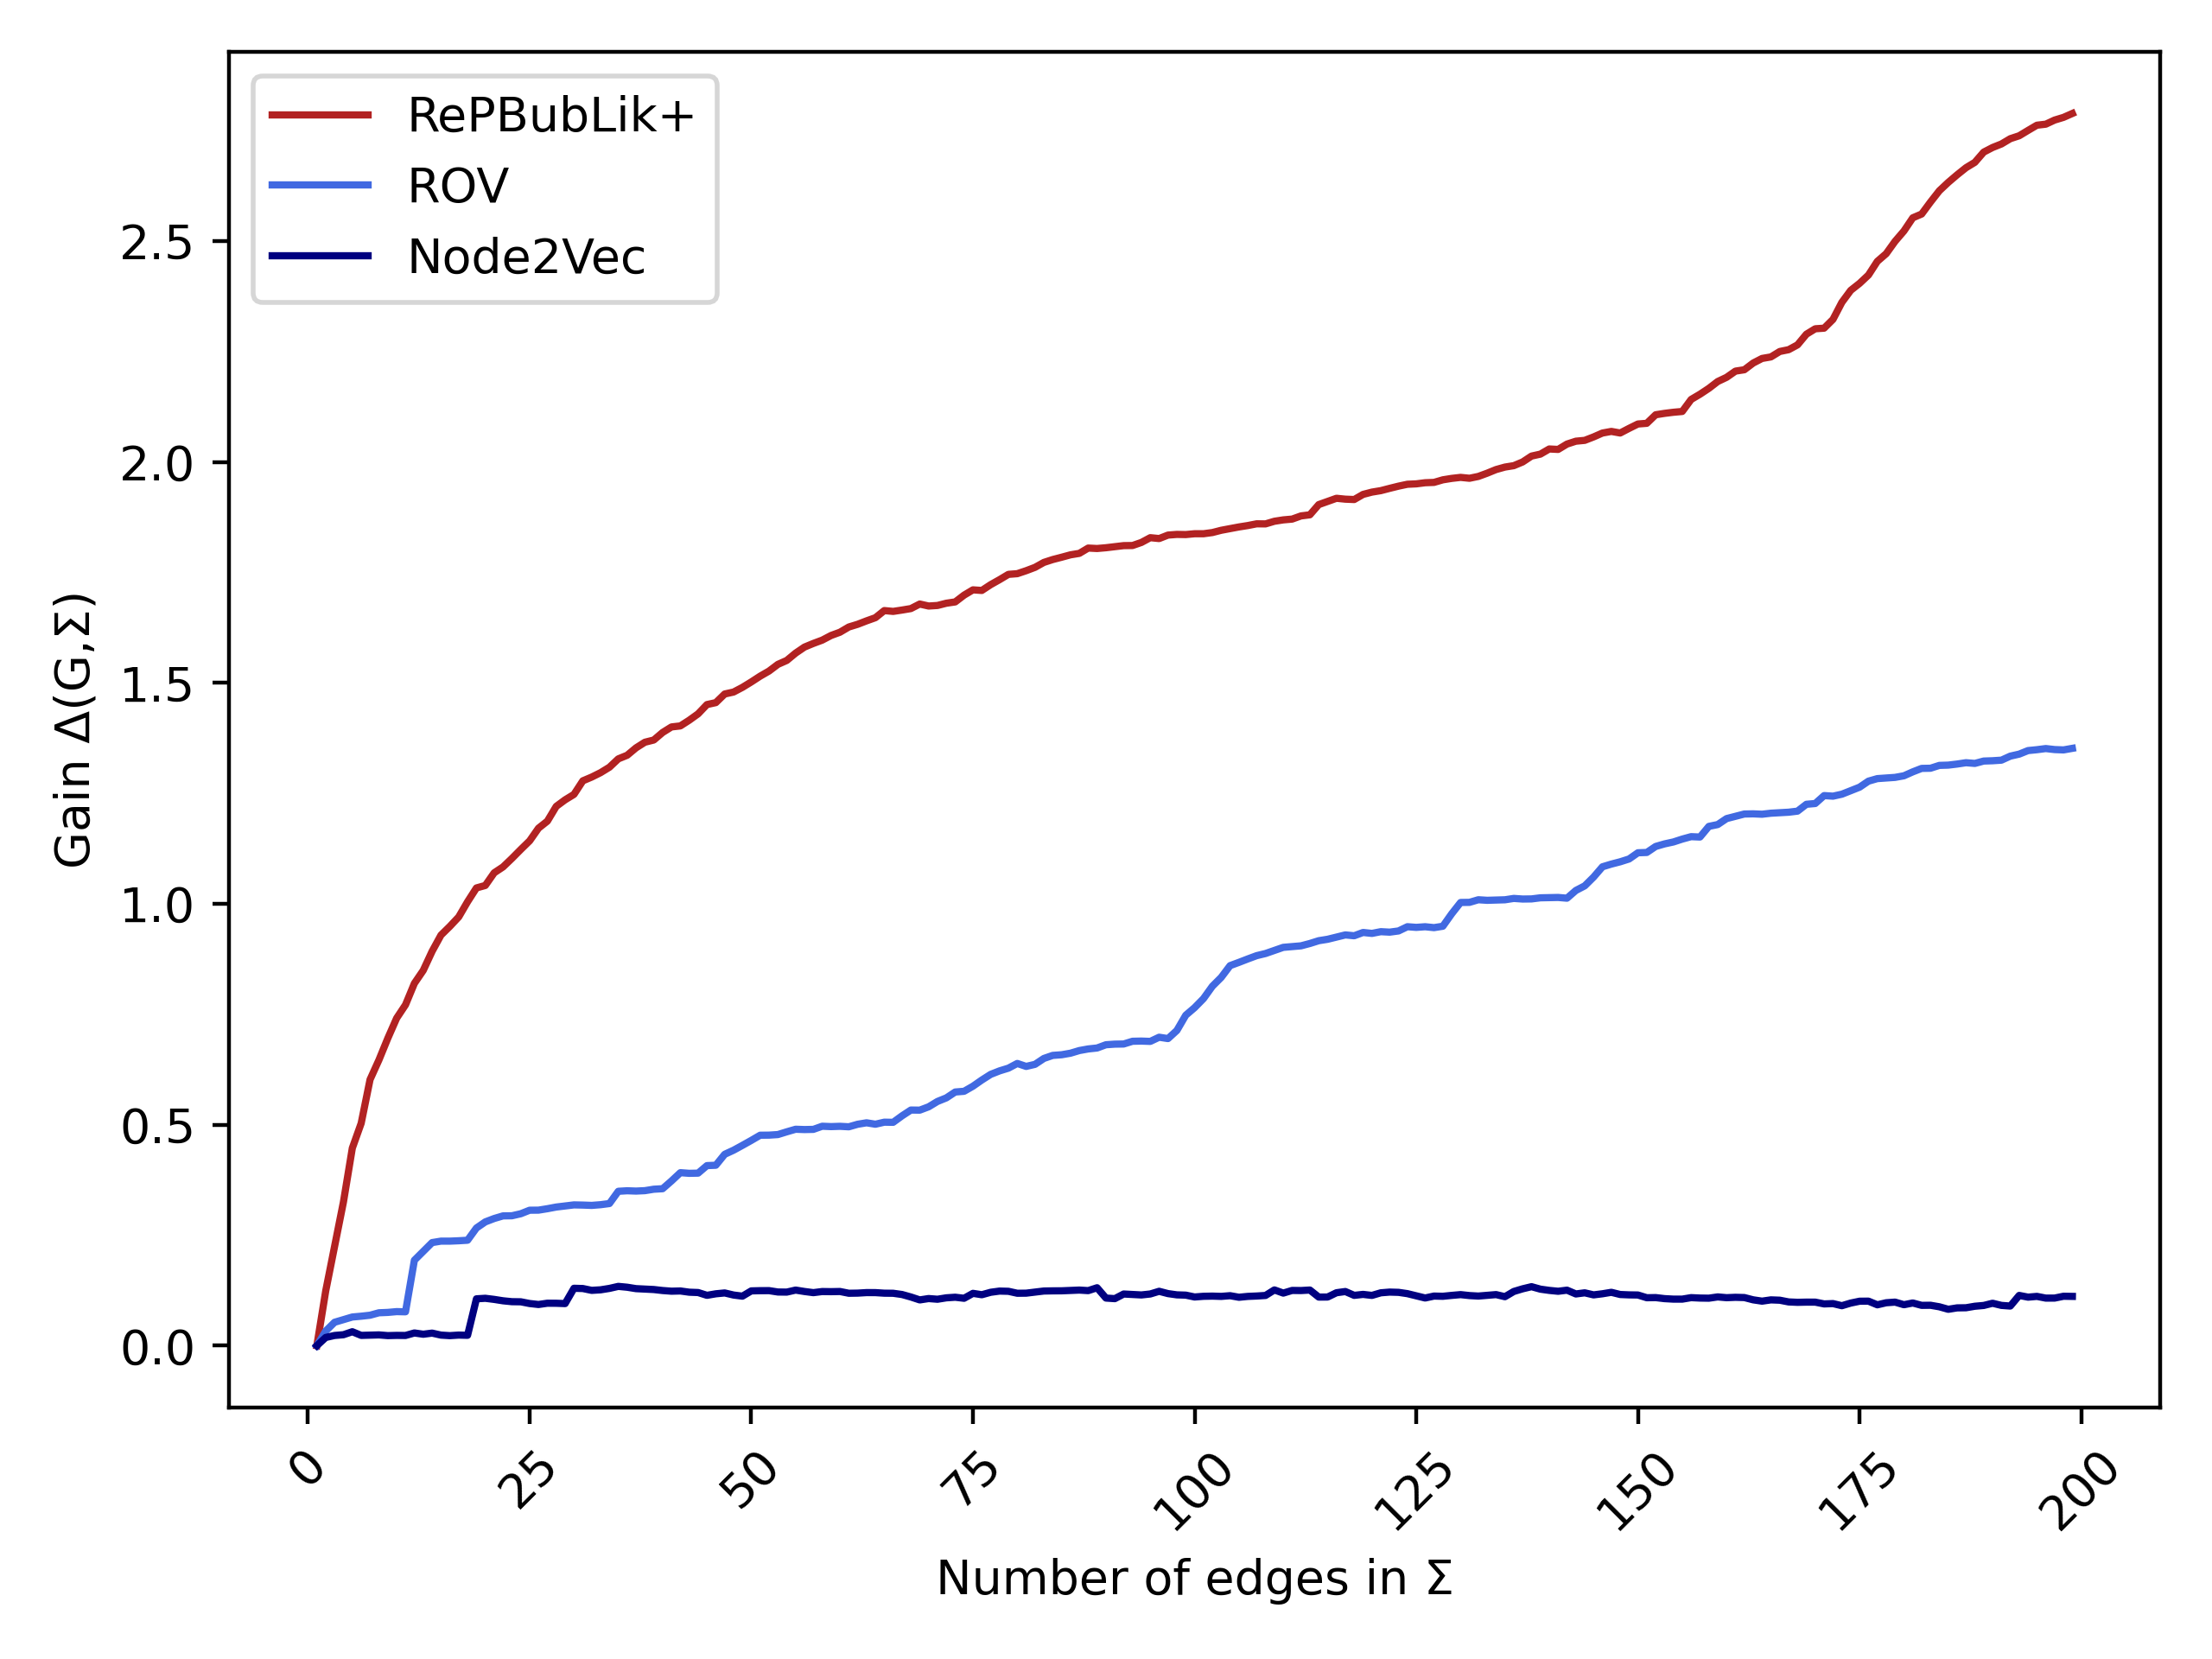
\includegraphics[width=\columnwidth]{10/polblogs_gain_10.png}
    \caption{\emph{PolBlogs} plot}\label{fig:polblogs_g_10}
\end{subfigure}
\caption{Grafici $\Delta(G,\Sigma)$ per $t=10$}
\end{figure}
\newpage
\begin{figure}[!h]
    \centering
\begin{subfigure}[b]{0.4\textwidth}
    \centering
    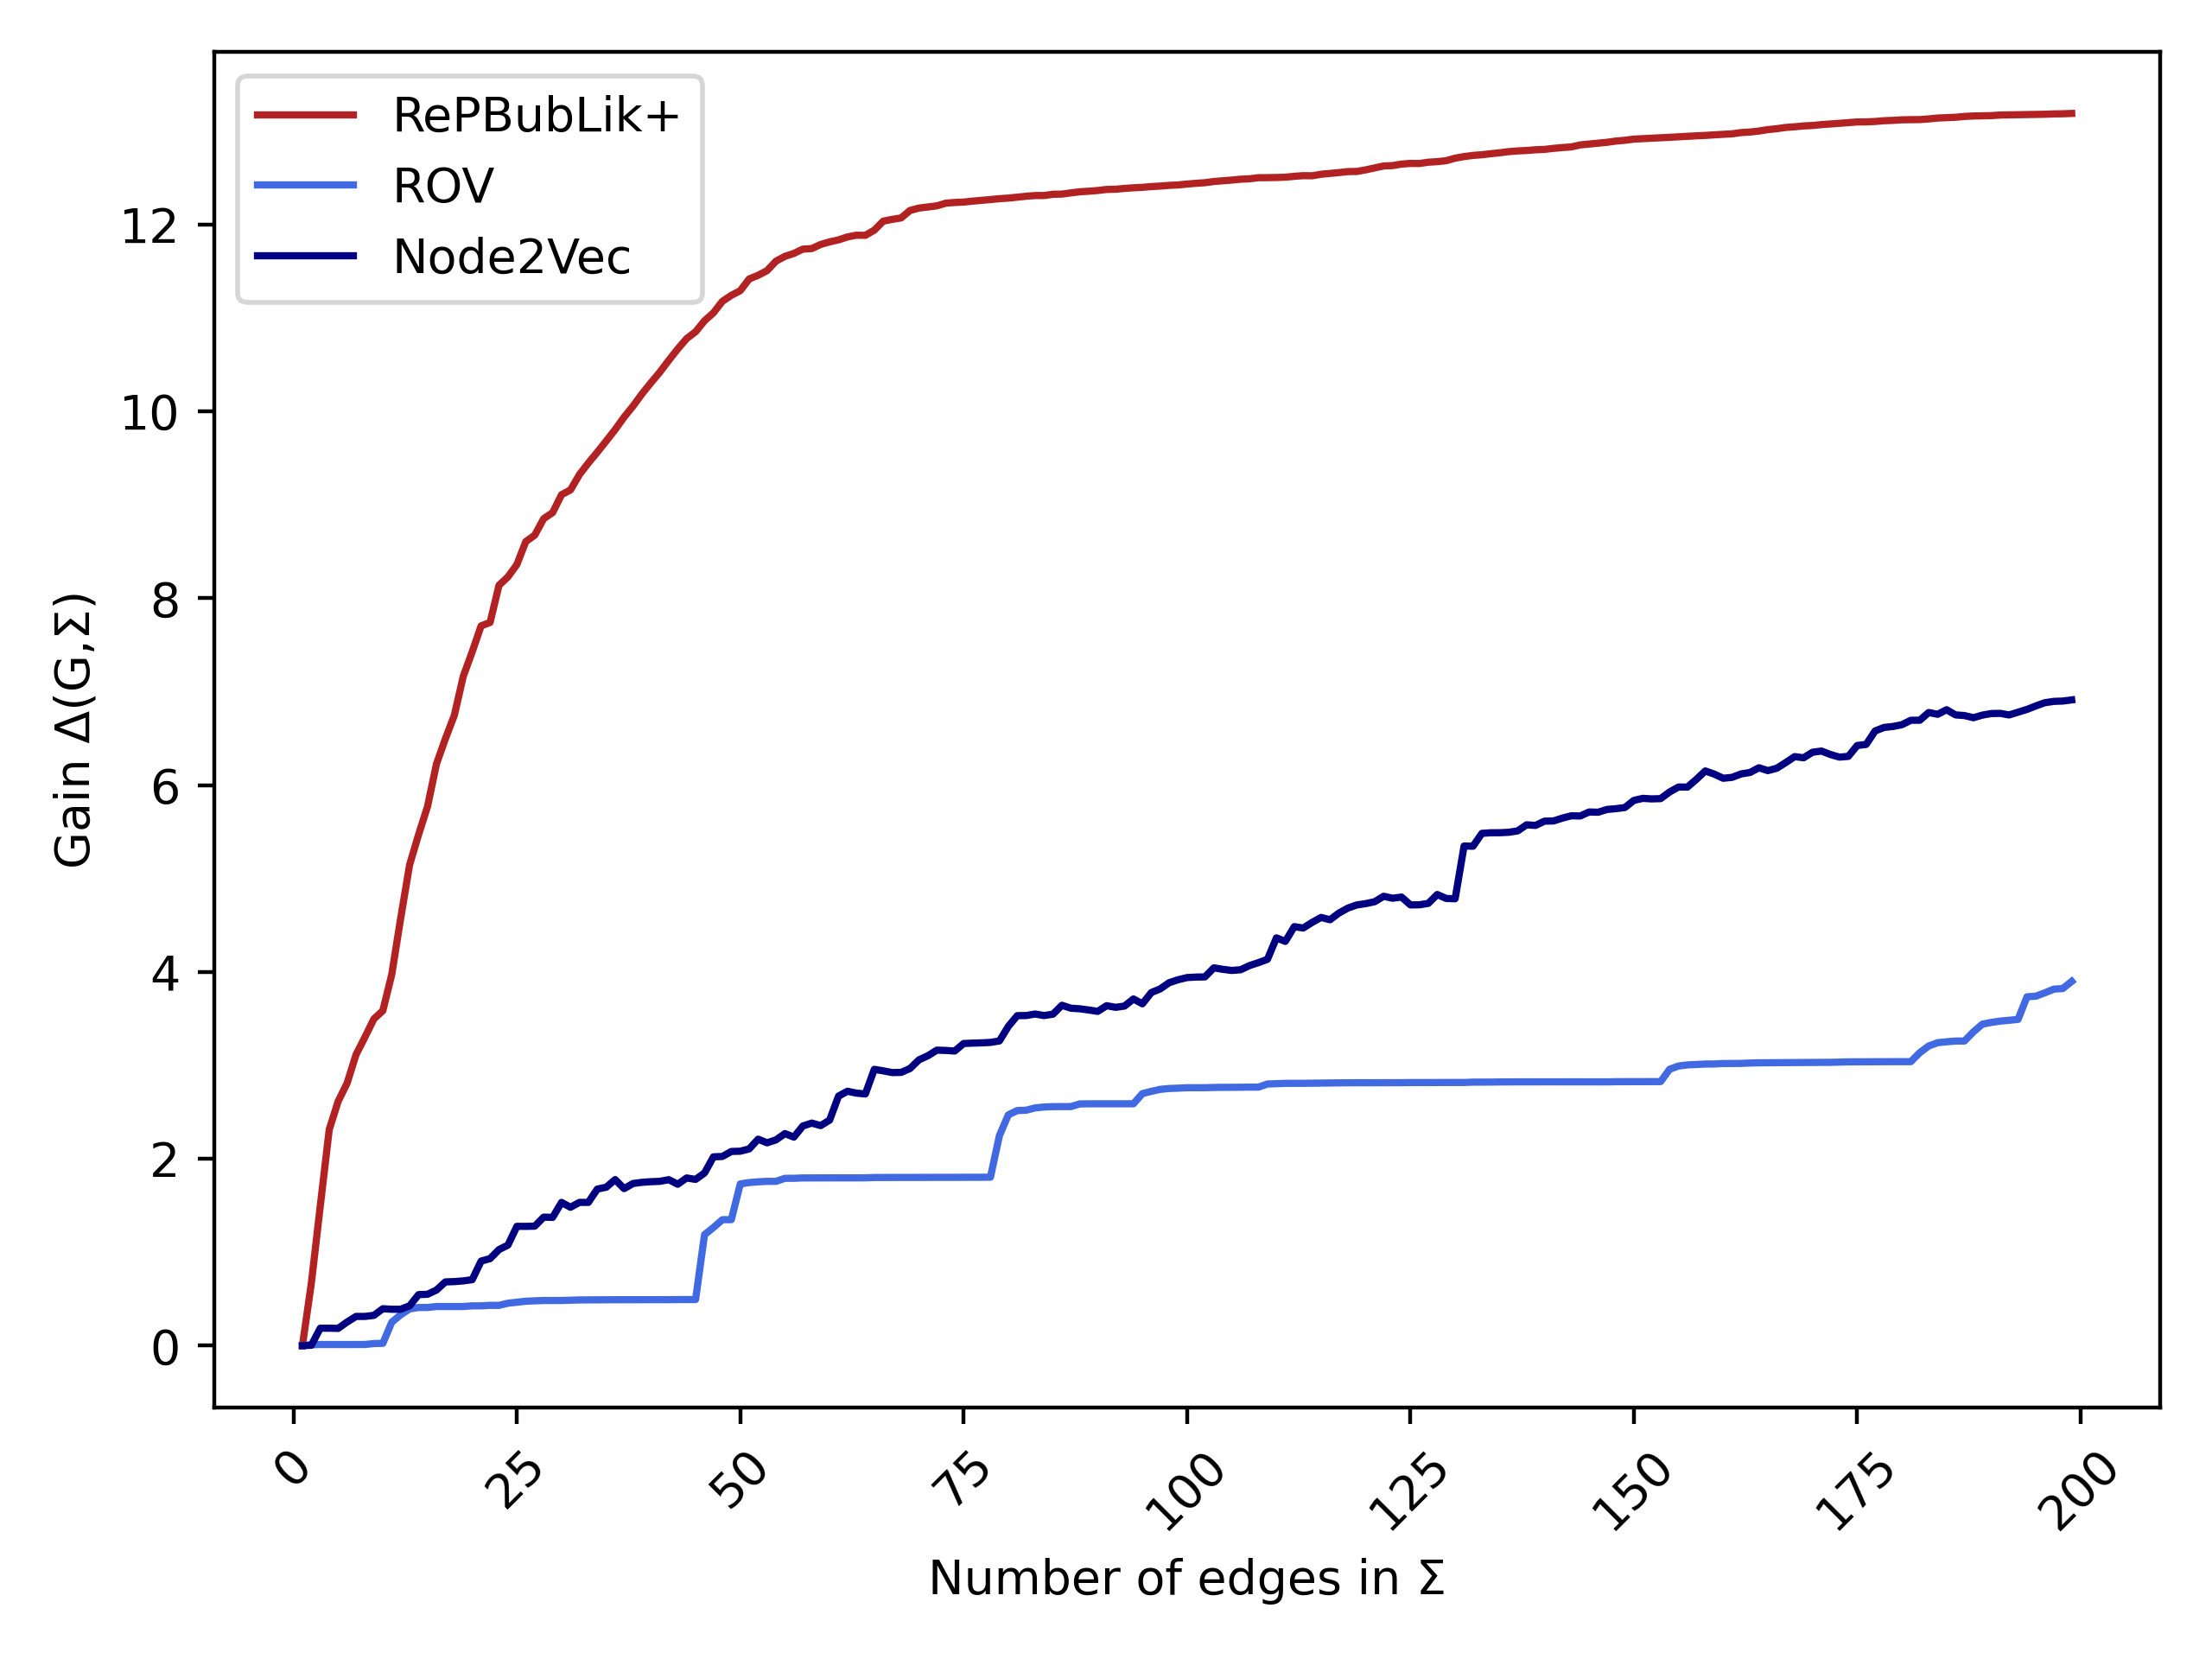
\includegraphics[width=\columnwidth]{15/math_tech_gain_15.png}
    \caption{\emph{MaTe} plot}\label{fig:mate_g_15}
\end{subfigure}
\hspace{0.1\columnwidth}
\begin{subfigure}[b]{0.4\textwidth}
    \centering
    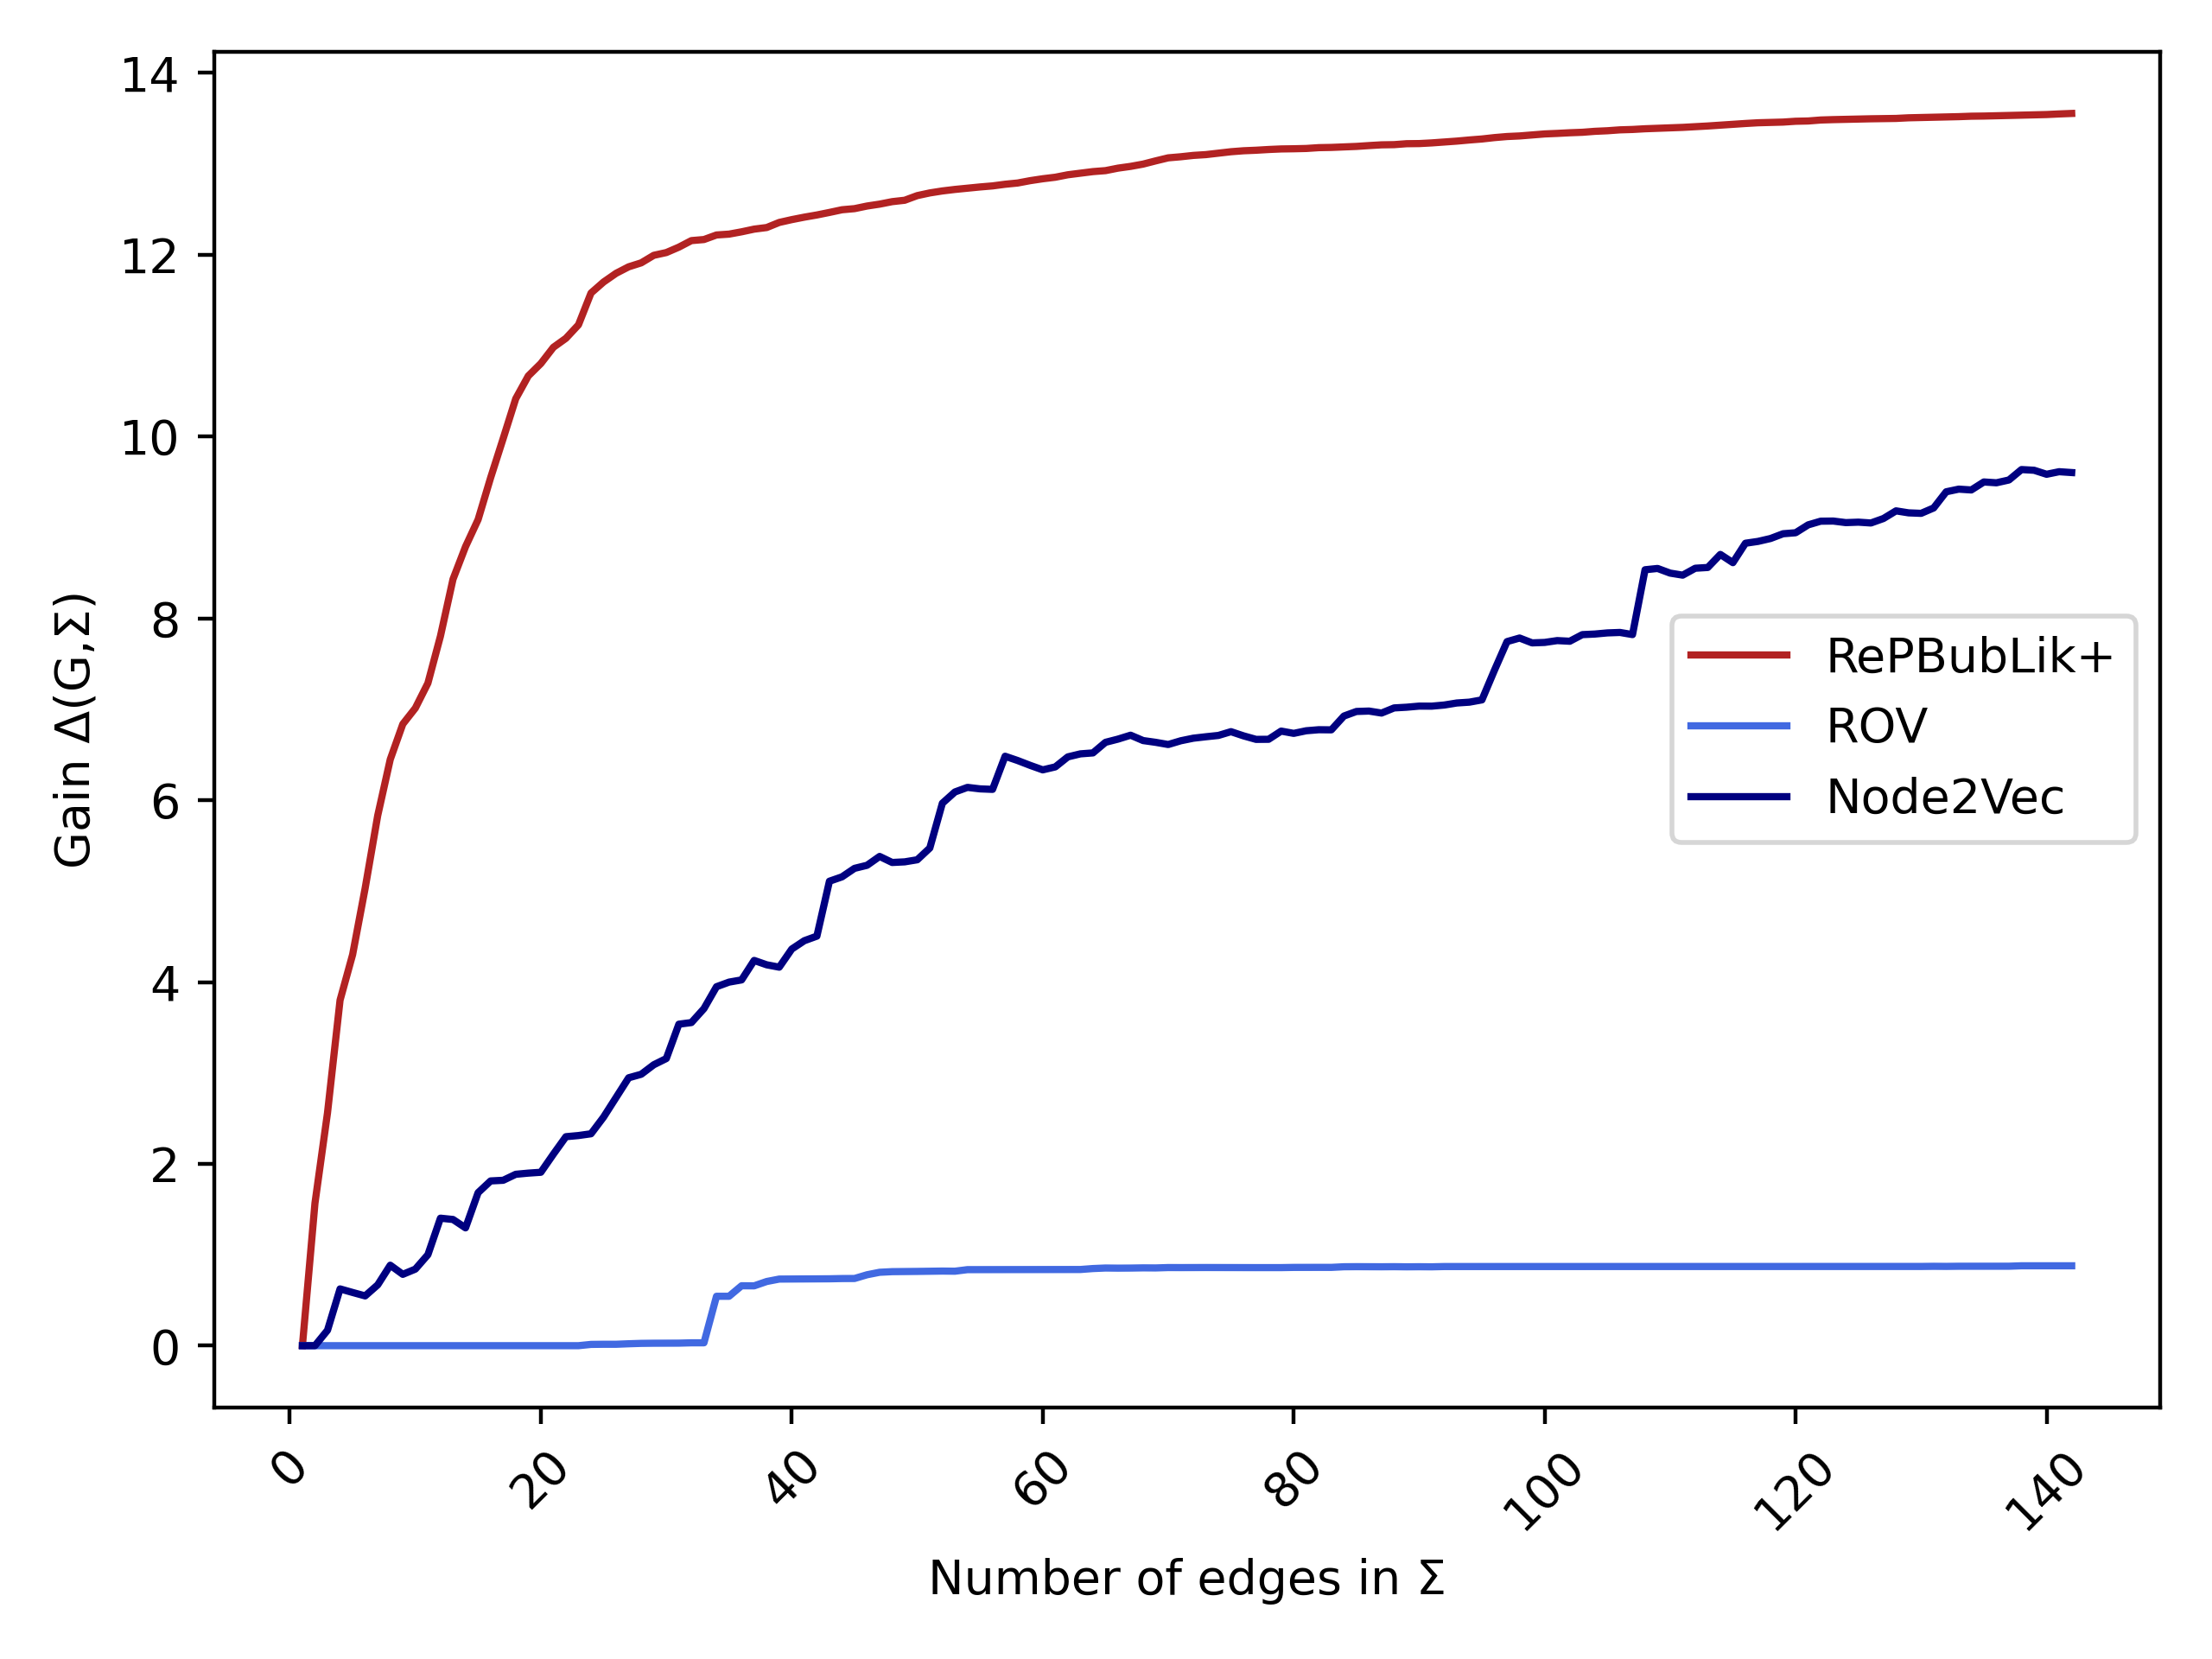
\includegraphics[width=\columnwidth]{15/tech_mil_gain_15.png}
    \caption{\emph{MiHi} plot}\label{fig:mihi_g_15}
\end{subfigure}

\begin{subfigure}[b]{0.4\textwidth}
    \centering
    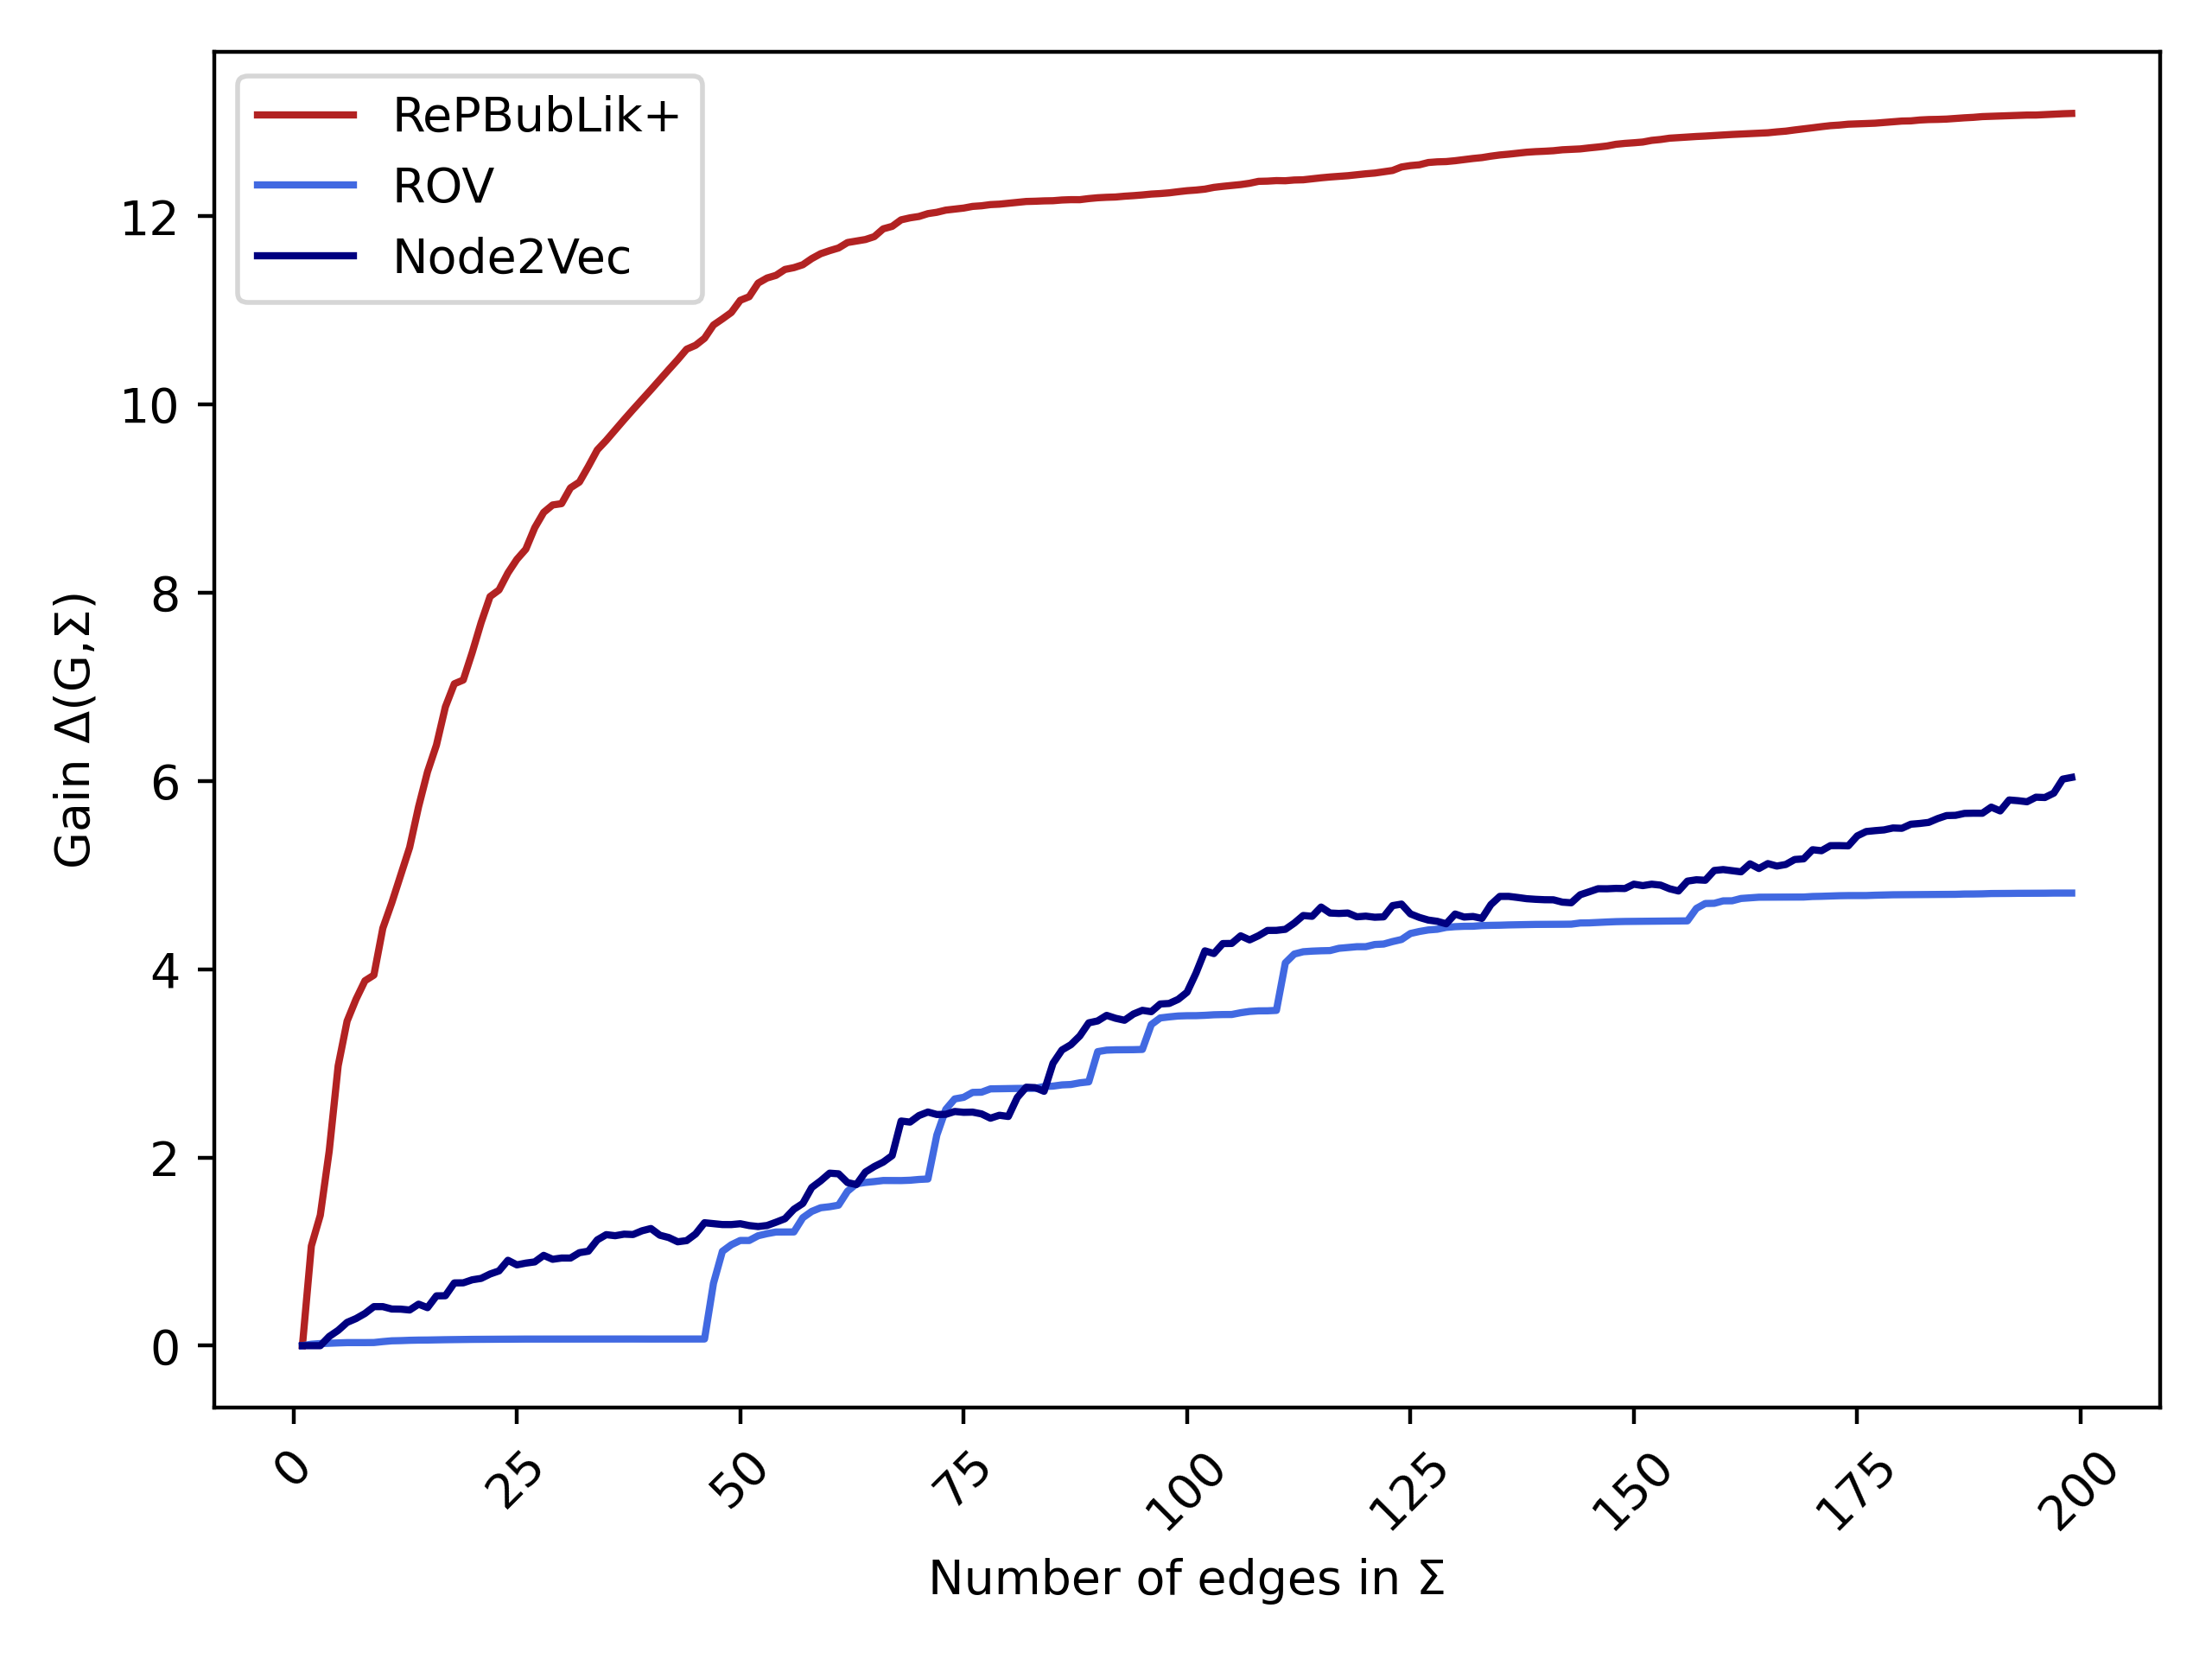
\includegraphics[width=\columnwidth]{15/math_ast_gain_15.png}
    \caption{\emph{MaA}s plot}\label{fig:maas_g_15}
\end{subfigure}
\hspace{0.1\columnwidth}
\begin{subfigure}[b]{0.4\textwidth}
    \centering
    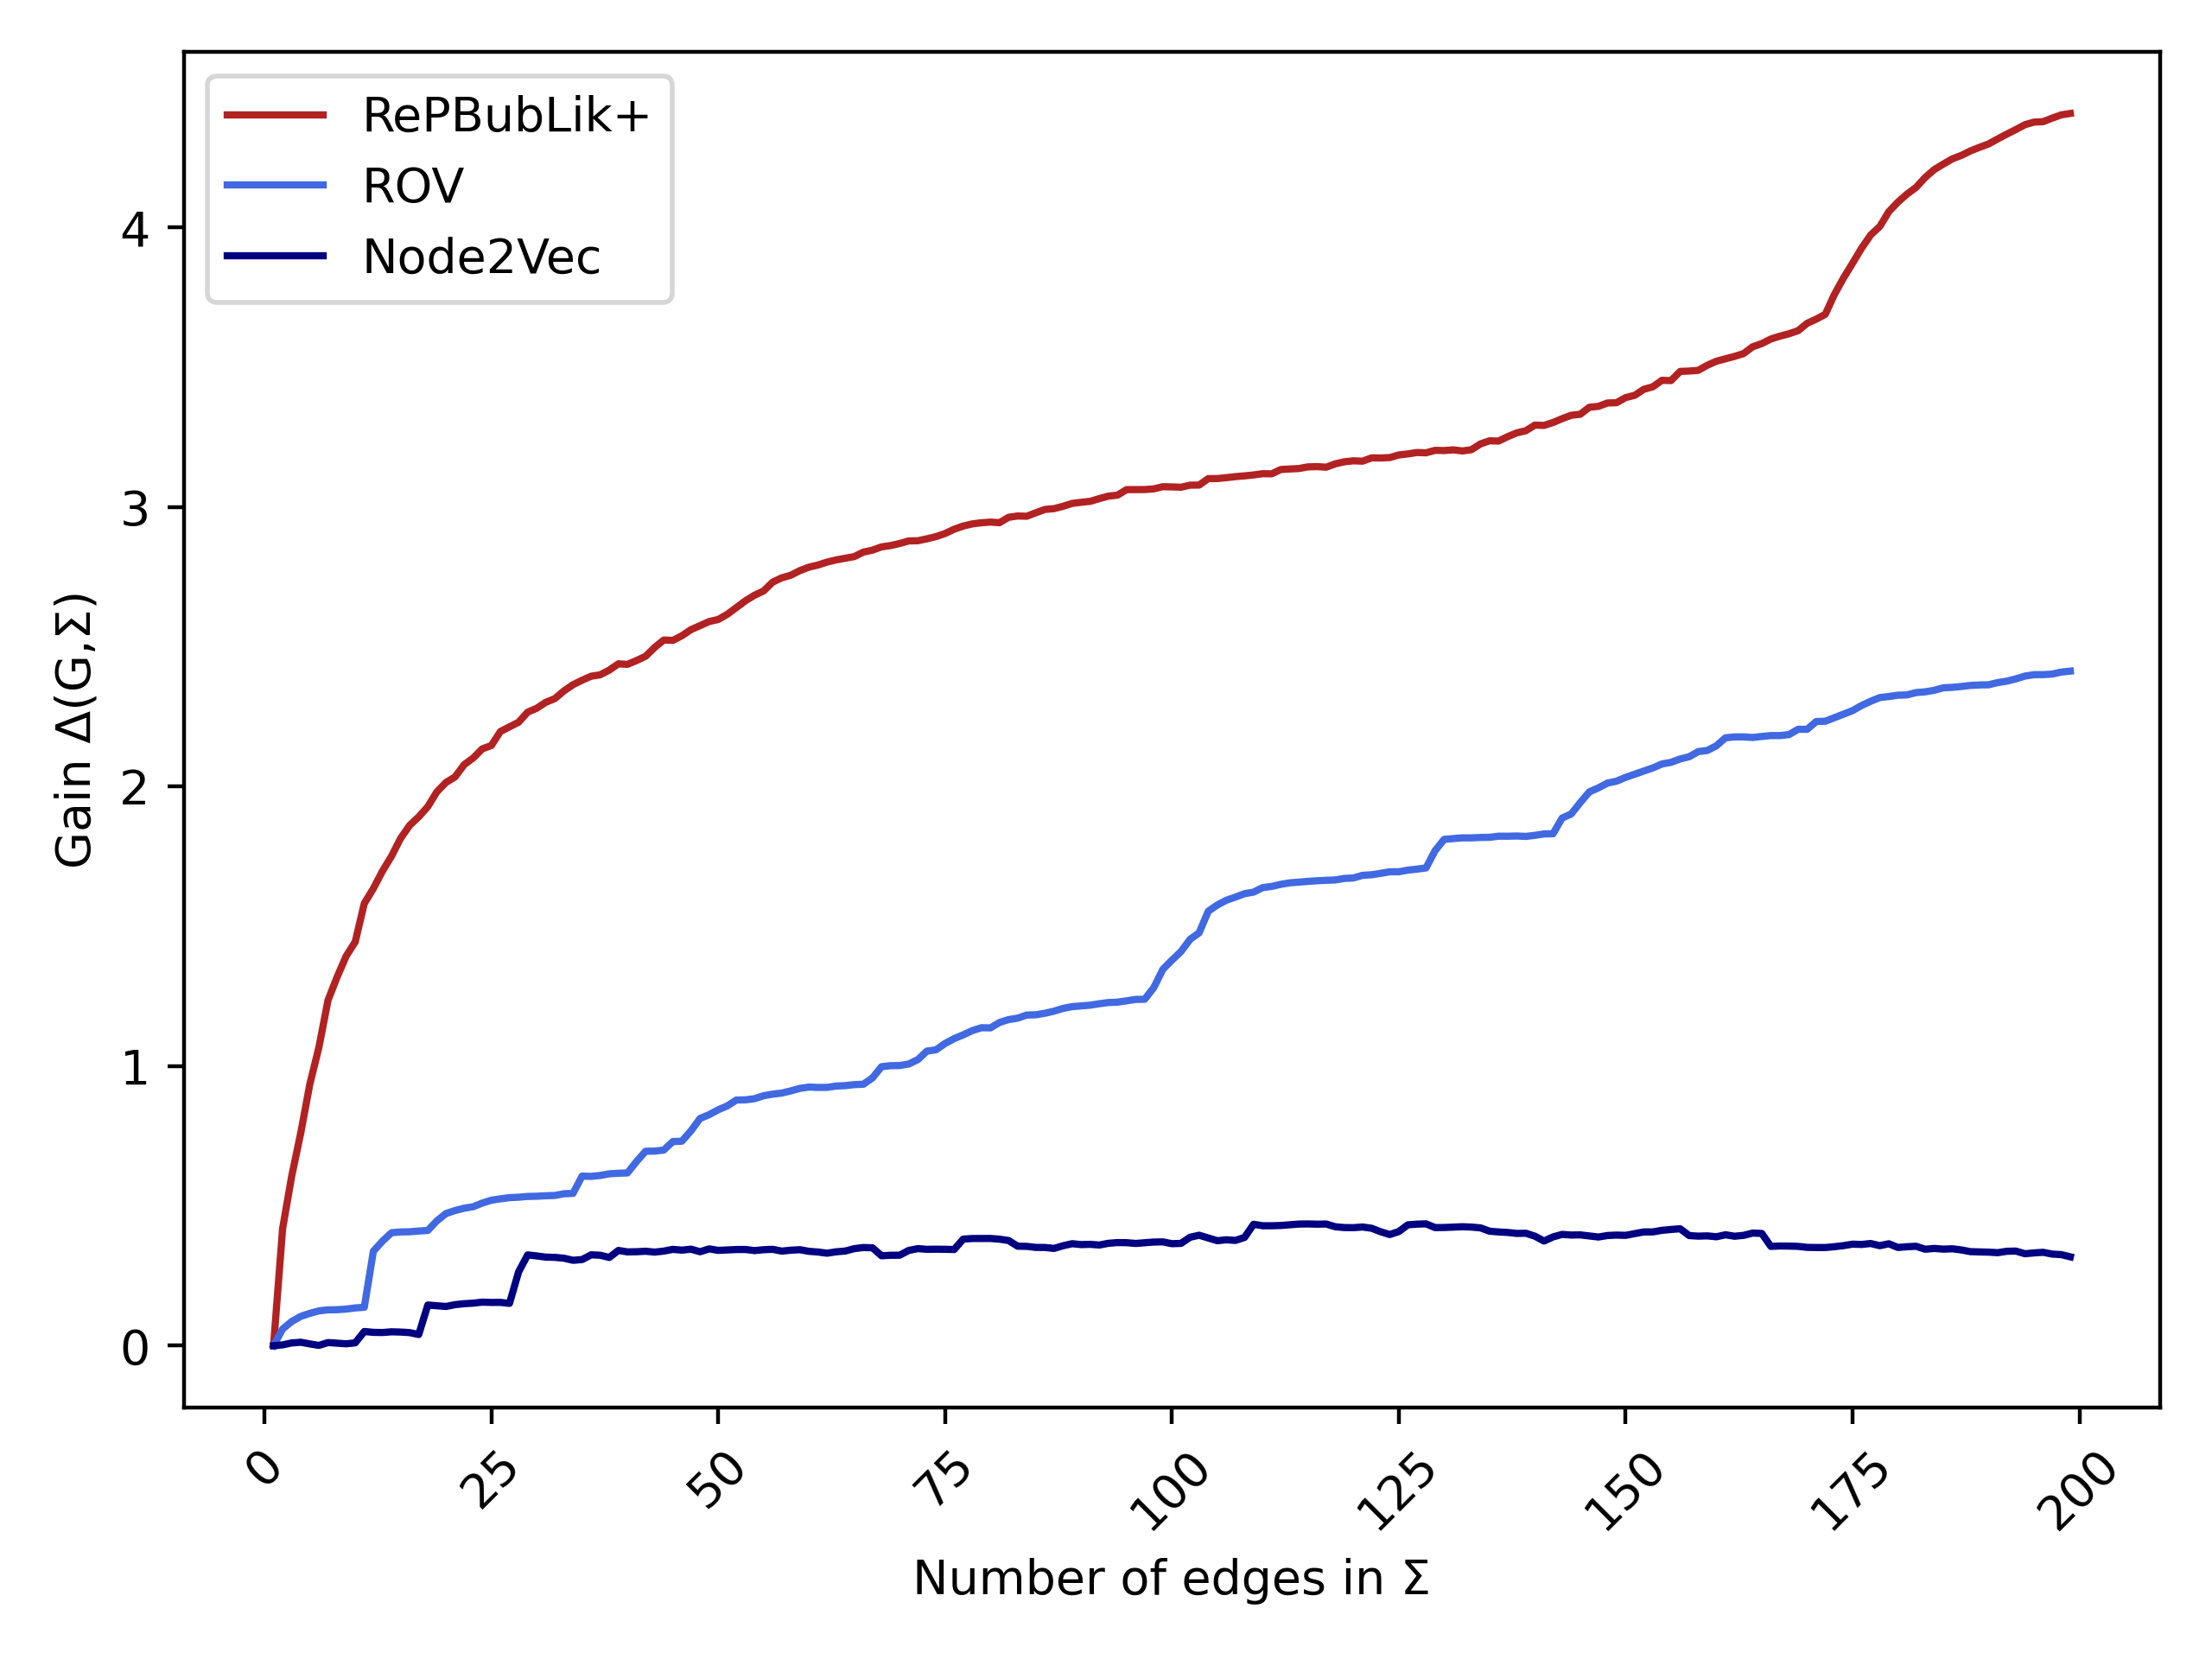
\includegraphics[width=\columnwidth]{15/polblogs_gain_15.png}
    \caption{\emph{PolBlogs} plot}\label{fig:polblogs_g_15}
\end{subfigure}
\caption{Grafici $\Delta(G,\Sigma)$ per $t=15$}
\end{figure}

Dai grafici dei guadagni, si evince che:
\begin{enumerate}
    \item RePBubLik+ è il migliore tra gli algoritmi proposti, in termini di guadagno $\Delta(G,\Sigma)$ rispetto al numero di archi in $\Sigma$.
    \item L'applicazione di RePBubLik+ a grafi di piccole dimensioni (\emph{MaTe}, \emph{MaAs}, \emph{MiHi}) porta ad un guadagno massimo maggiore rispetto a quello ottenuto mediante gli algoritmi ROV e Node2Vec (es. (\emph{MaAs}) ${\Delta_{R+}\over{\Delta_{ROV}}}=2.93$, ${\Delta_{R+}\over{\Delta_{Node2Vec}}}=2.56$ per $k=200,t=10$).
    \item L'applicazione di RePBubLik+ a grafi di medie dimensioni (\emph{PolBlogs}) porta ad un guadagno massimo maggiore rispetto a quello ottenuto mediante gli algoritmi ROV e Node2Vec (es. (\emph{PolBlogs}) ${\Delta_{R+}\over{\Delta_{ROV}}}=2.34$, ${\Delta_{R+}\over{\Delta_{Node2Vec}}}=18.67$ per  $k=200,t=10$).
    \item RePBubLik+ risulta essere il miglior algoritmo in quanto per un numero ridotto di archi riporta un notevole guadagno: nei grafici sovrastanti, la curva dell'algoritmo RePBubLik+ cresce molto rapidamente per valori piccoli di $k$, raggiungendo una plateau per un certo valore di $\Delta(G,\Sigma)$.
            Questo, dal punto di vista pratico, è molto interessante perchè permette con pochi archi aggiuntivi di ridurre notevolmente la polarizzazione in grafi simili a quelli presi in esame (es. (\emph{MaTe}) ${\Delta_{R+}\over{\Delta_{ROV}}}=7.45$, ${\Delta_{R+}\over{\Delta_{Node2Vec}}}=3.35$ per $k=50,t=10$).
    \item Le considerazioni fatte nei punti precedenti sono generalmente valide, per qualsiasi valore di $t$ e qualsiasi grafo. Valutando i guadagni dei grafi anche in termini di RW massimo, si può notare che per valori di $t$ maggiori, RePBubLik+ raggiunge il plateau con un numero inferiore d'archi (es. (\emph{MaTe}) $\Delta_{R+}=2$ per $k=50, t=5$,  $\Delta_{R+}=6.75$ per $k=50,t=10$, $\Delta_{R+}=11.5$ per $k=50,t=15$).
\end{enumerate}
\subsection{Bias strutturale $\rho(G)$}
L'ultima metrica che viene anlizzata è il il bias $\rho(G)$ (\ref{REP:bias}) in relazione al numero 
degli archi aggiunti al grafo $G$. Lo studio di questa misura è interessante, in quanto permette di valutare il cambiamento della polarizzazione del grafo $G$.
\\
Di seguito i bias per ciascun grafo e per ciascun valore di $t$.

\begin{figure}[!h]
    \centering
\begin{subfigure}[b]{0.4\textwidth}
    \centering
    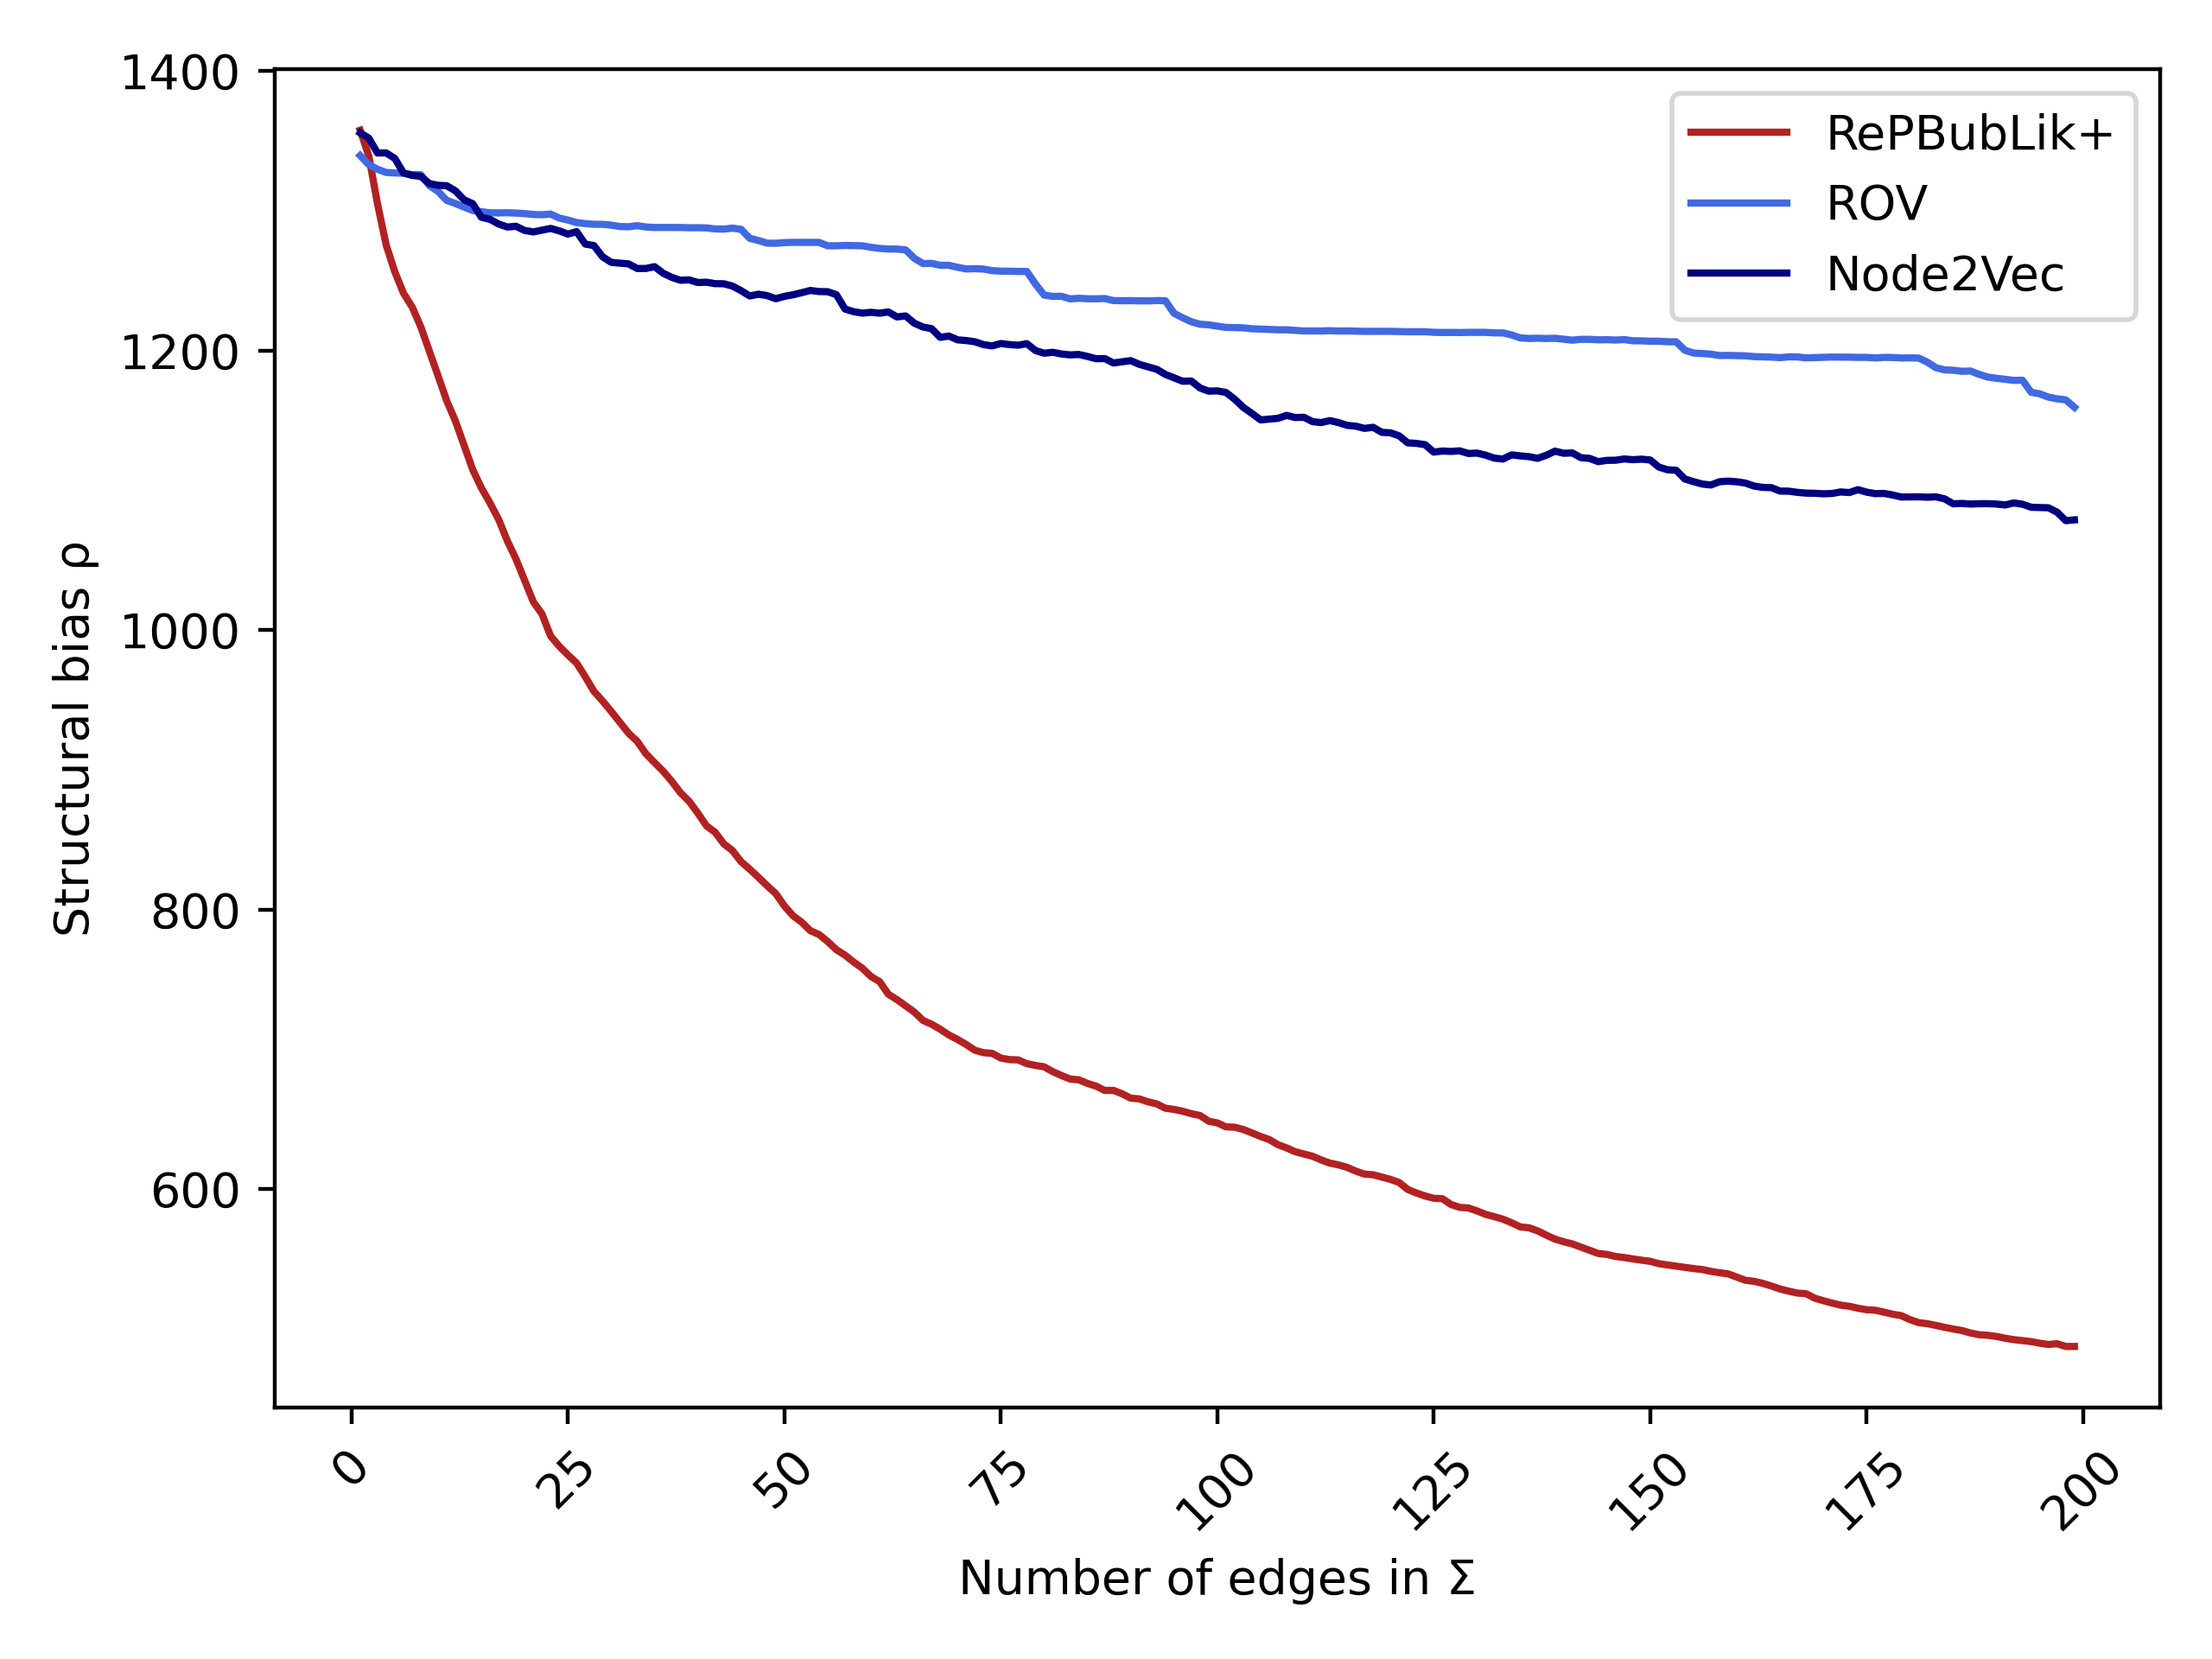
\includegraphics[width=\columnwidth]{5/math_tech_bias_5.png}
    \caption{\emph{MaTe} plot}\label{fig:mate_b_5}
\end{subfigure}
\hspace{0.1\columnwidth}
\begin{subfigure}[b]{0.4\textwidth}
    \centering
    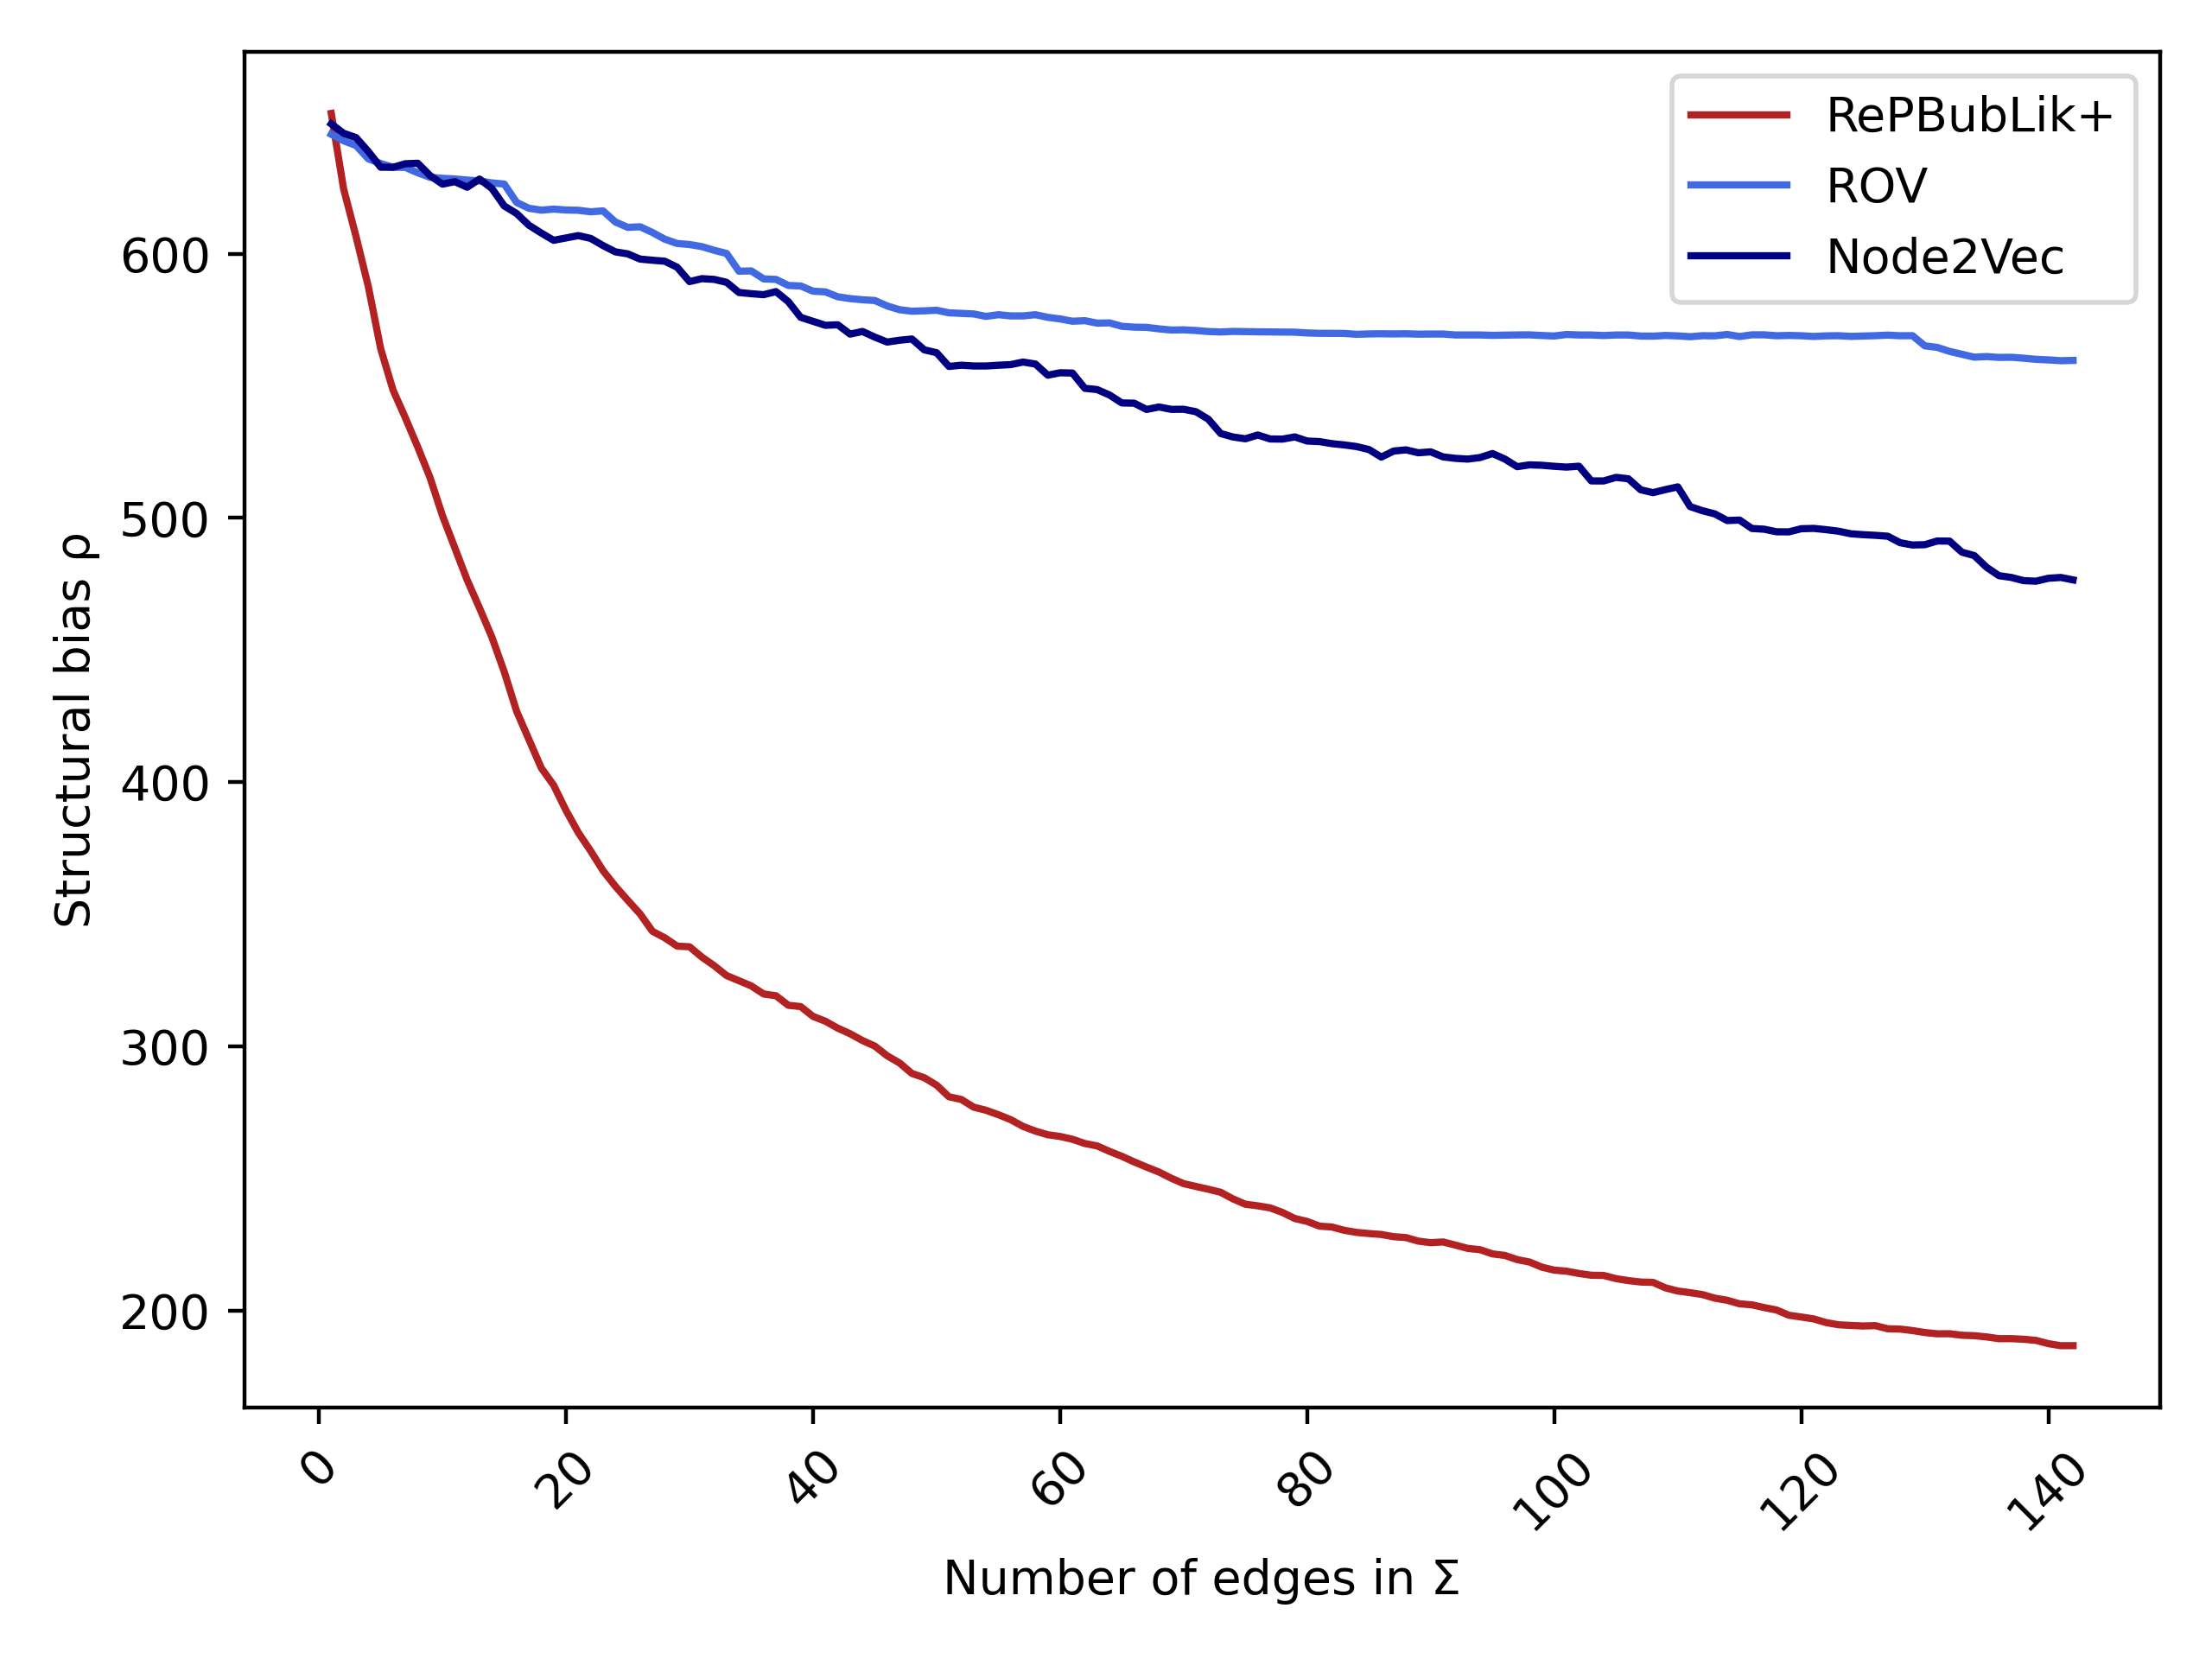
\includegraphics[width=\columnwidth]{5/tech_mil_bias_5.png}
    \caption{\emph{MiHi} plot}\label{fig:mihi_b_5}
\end{subfigure}

\begin{subfigure}[b]{0.4\textwidth}
    \centering
    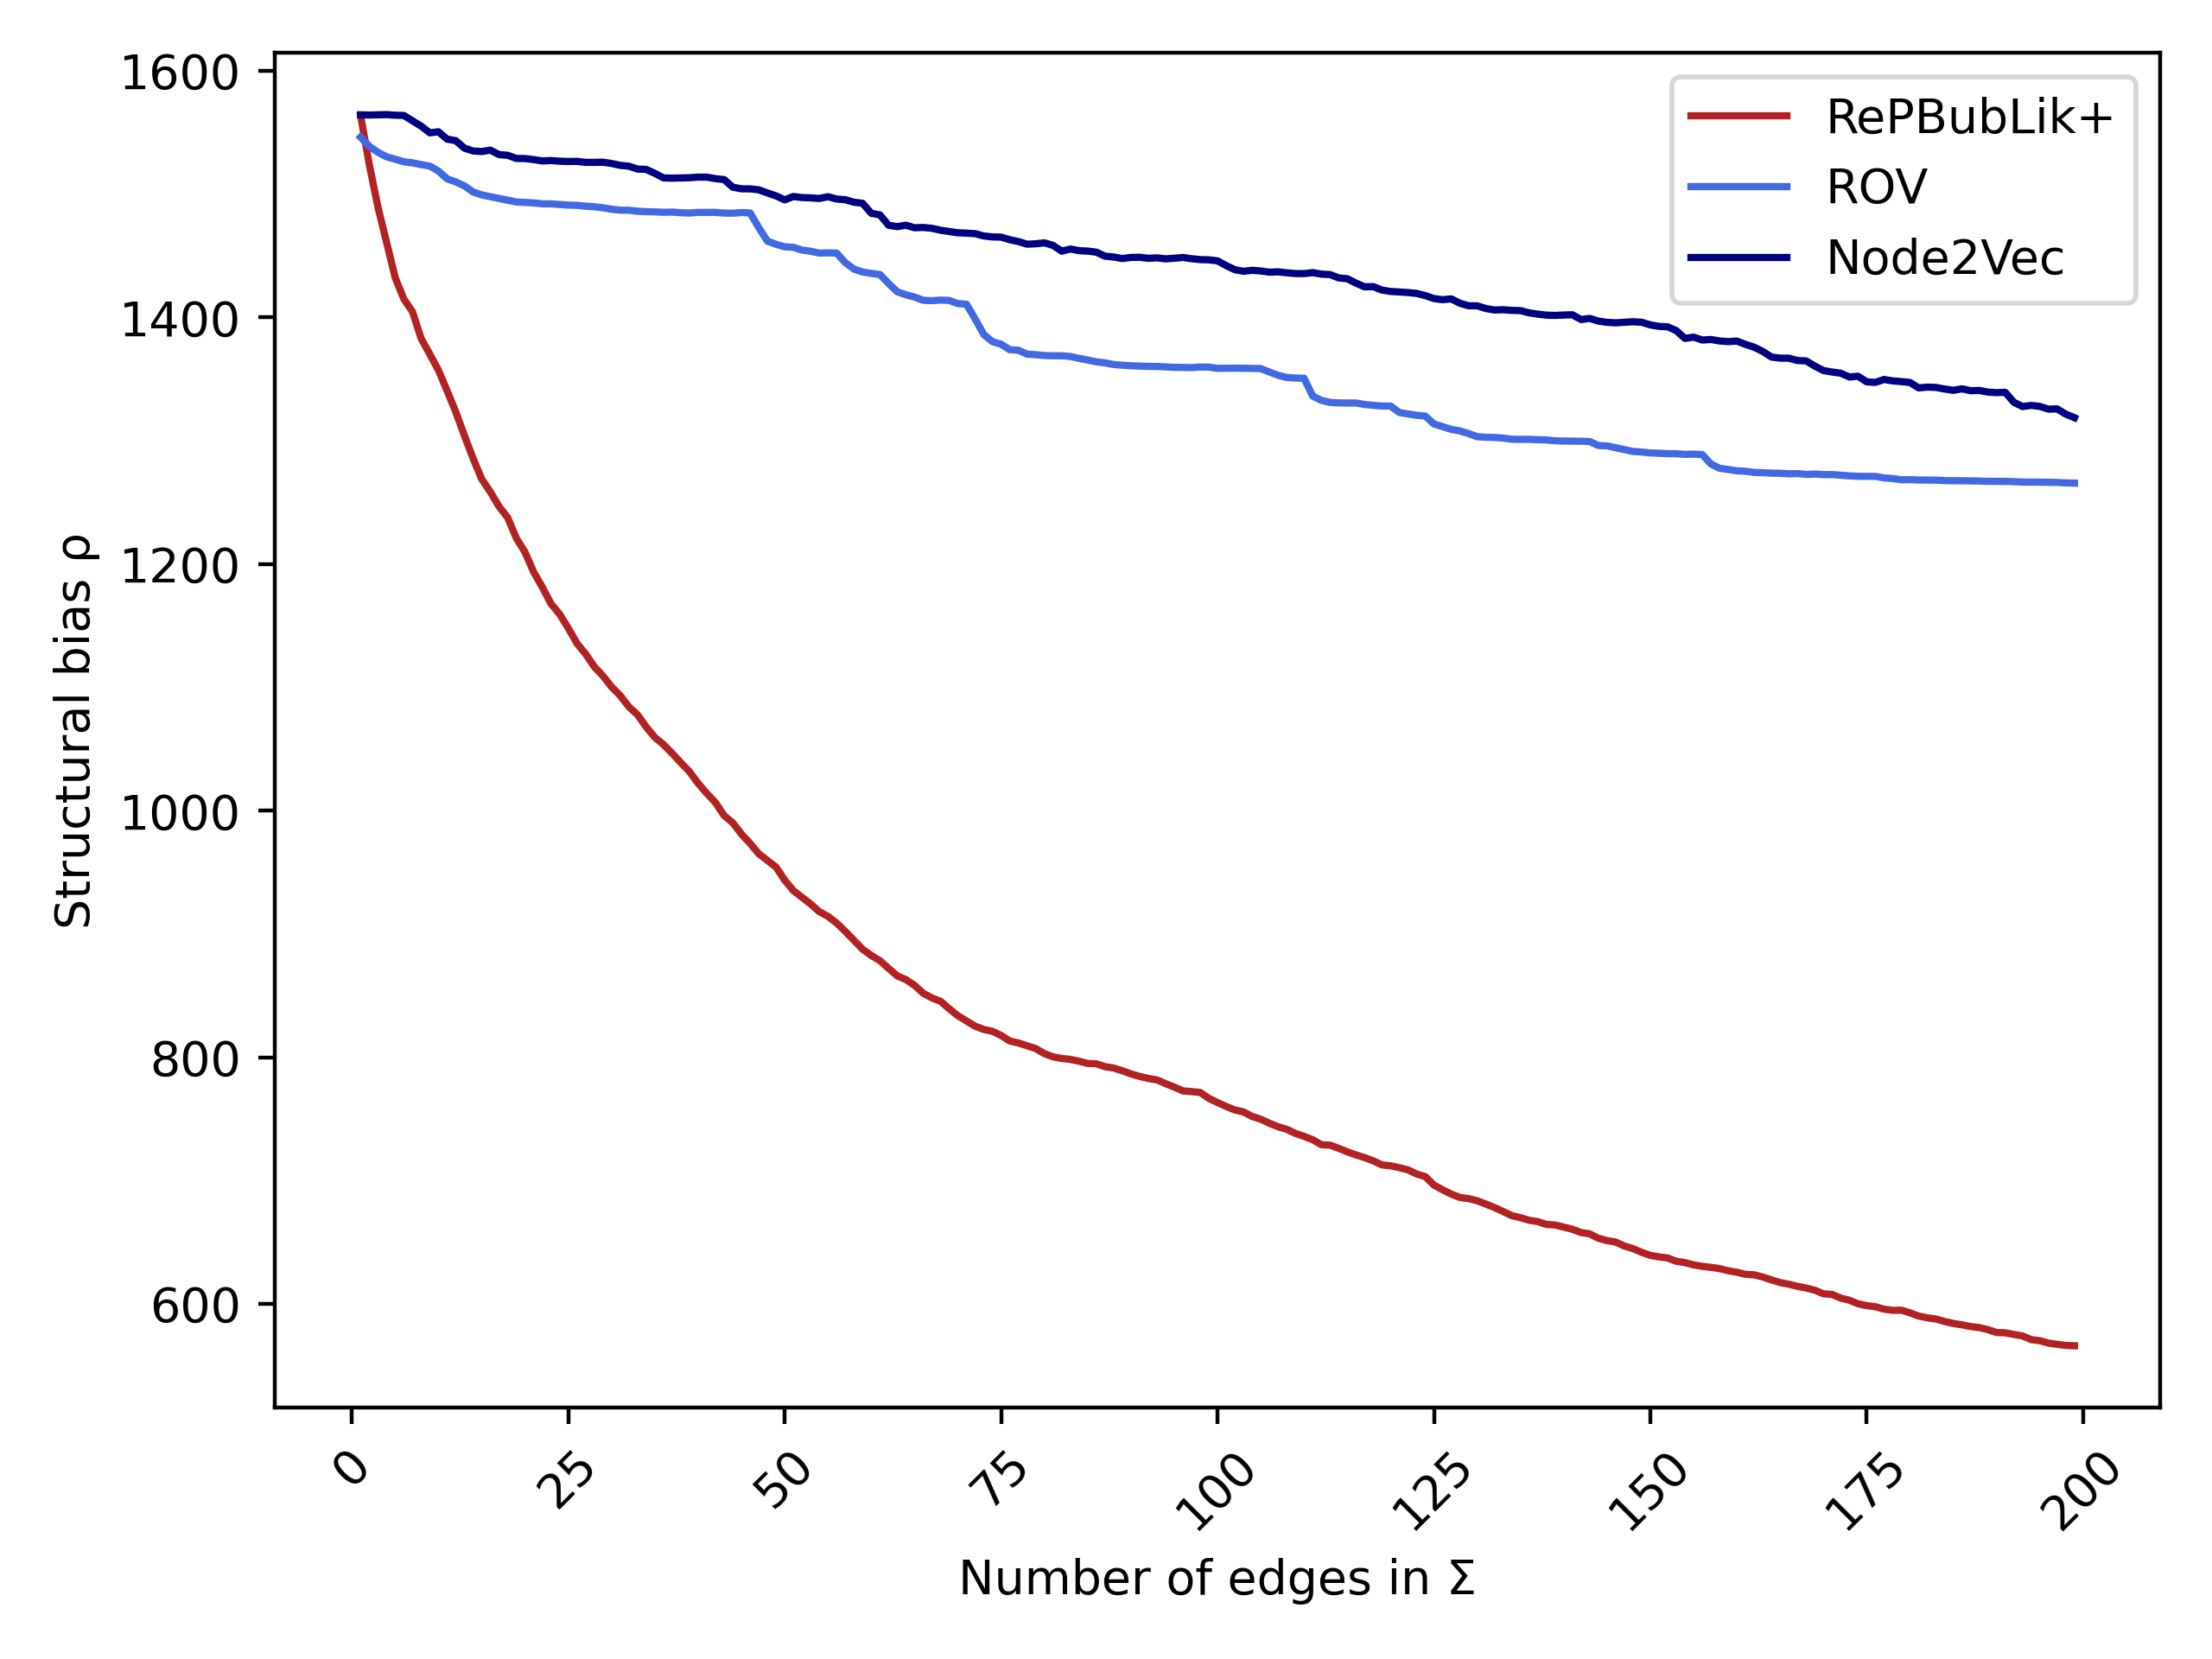
\includegraphics[width=\columnwidth]{5/math_ast_bias_5.png}
    \caption{\emph{MaA}s plot}\label{fig:maas_b_5}
\end{subfigure}
\hspace{0.1\columnwidth}
\begin{subfigure}[b]{0.4\textwidth}
    \centering
    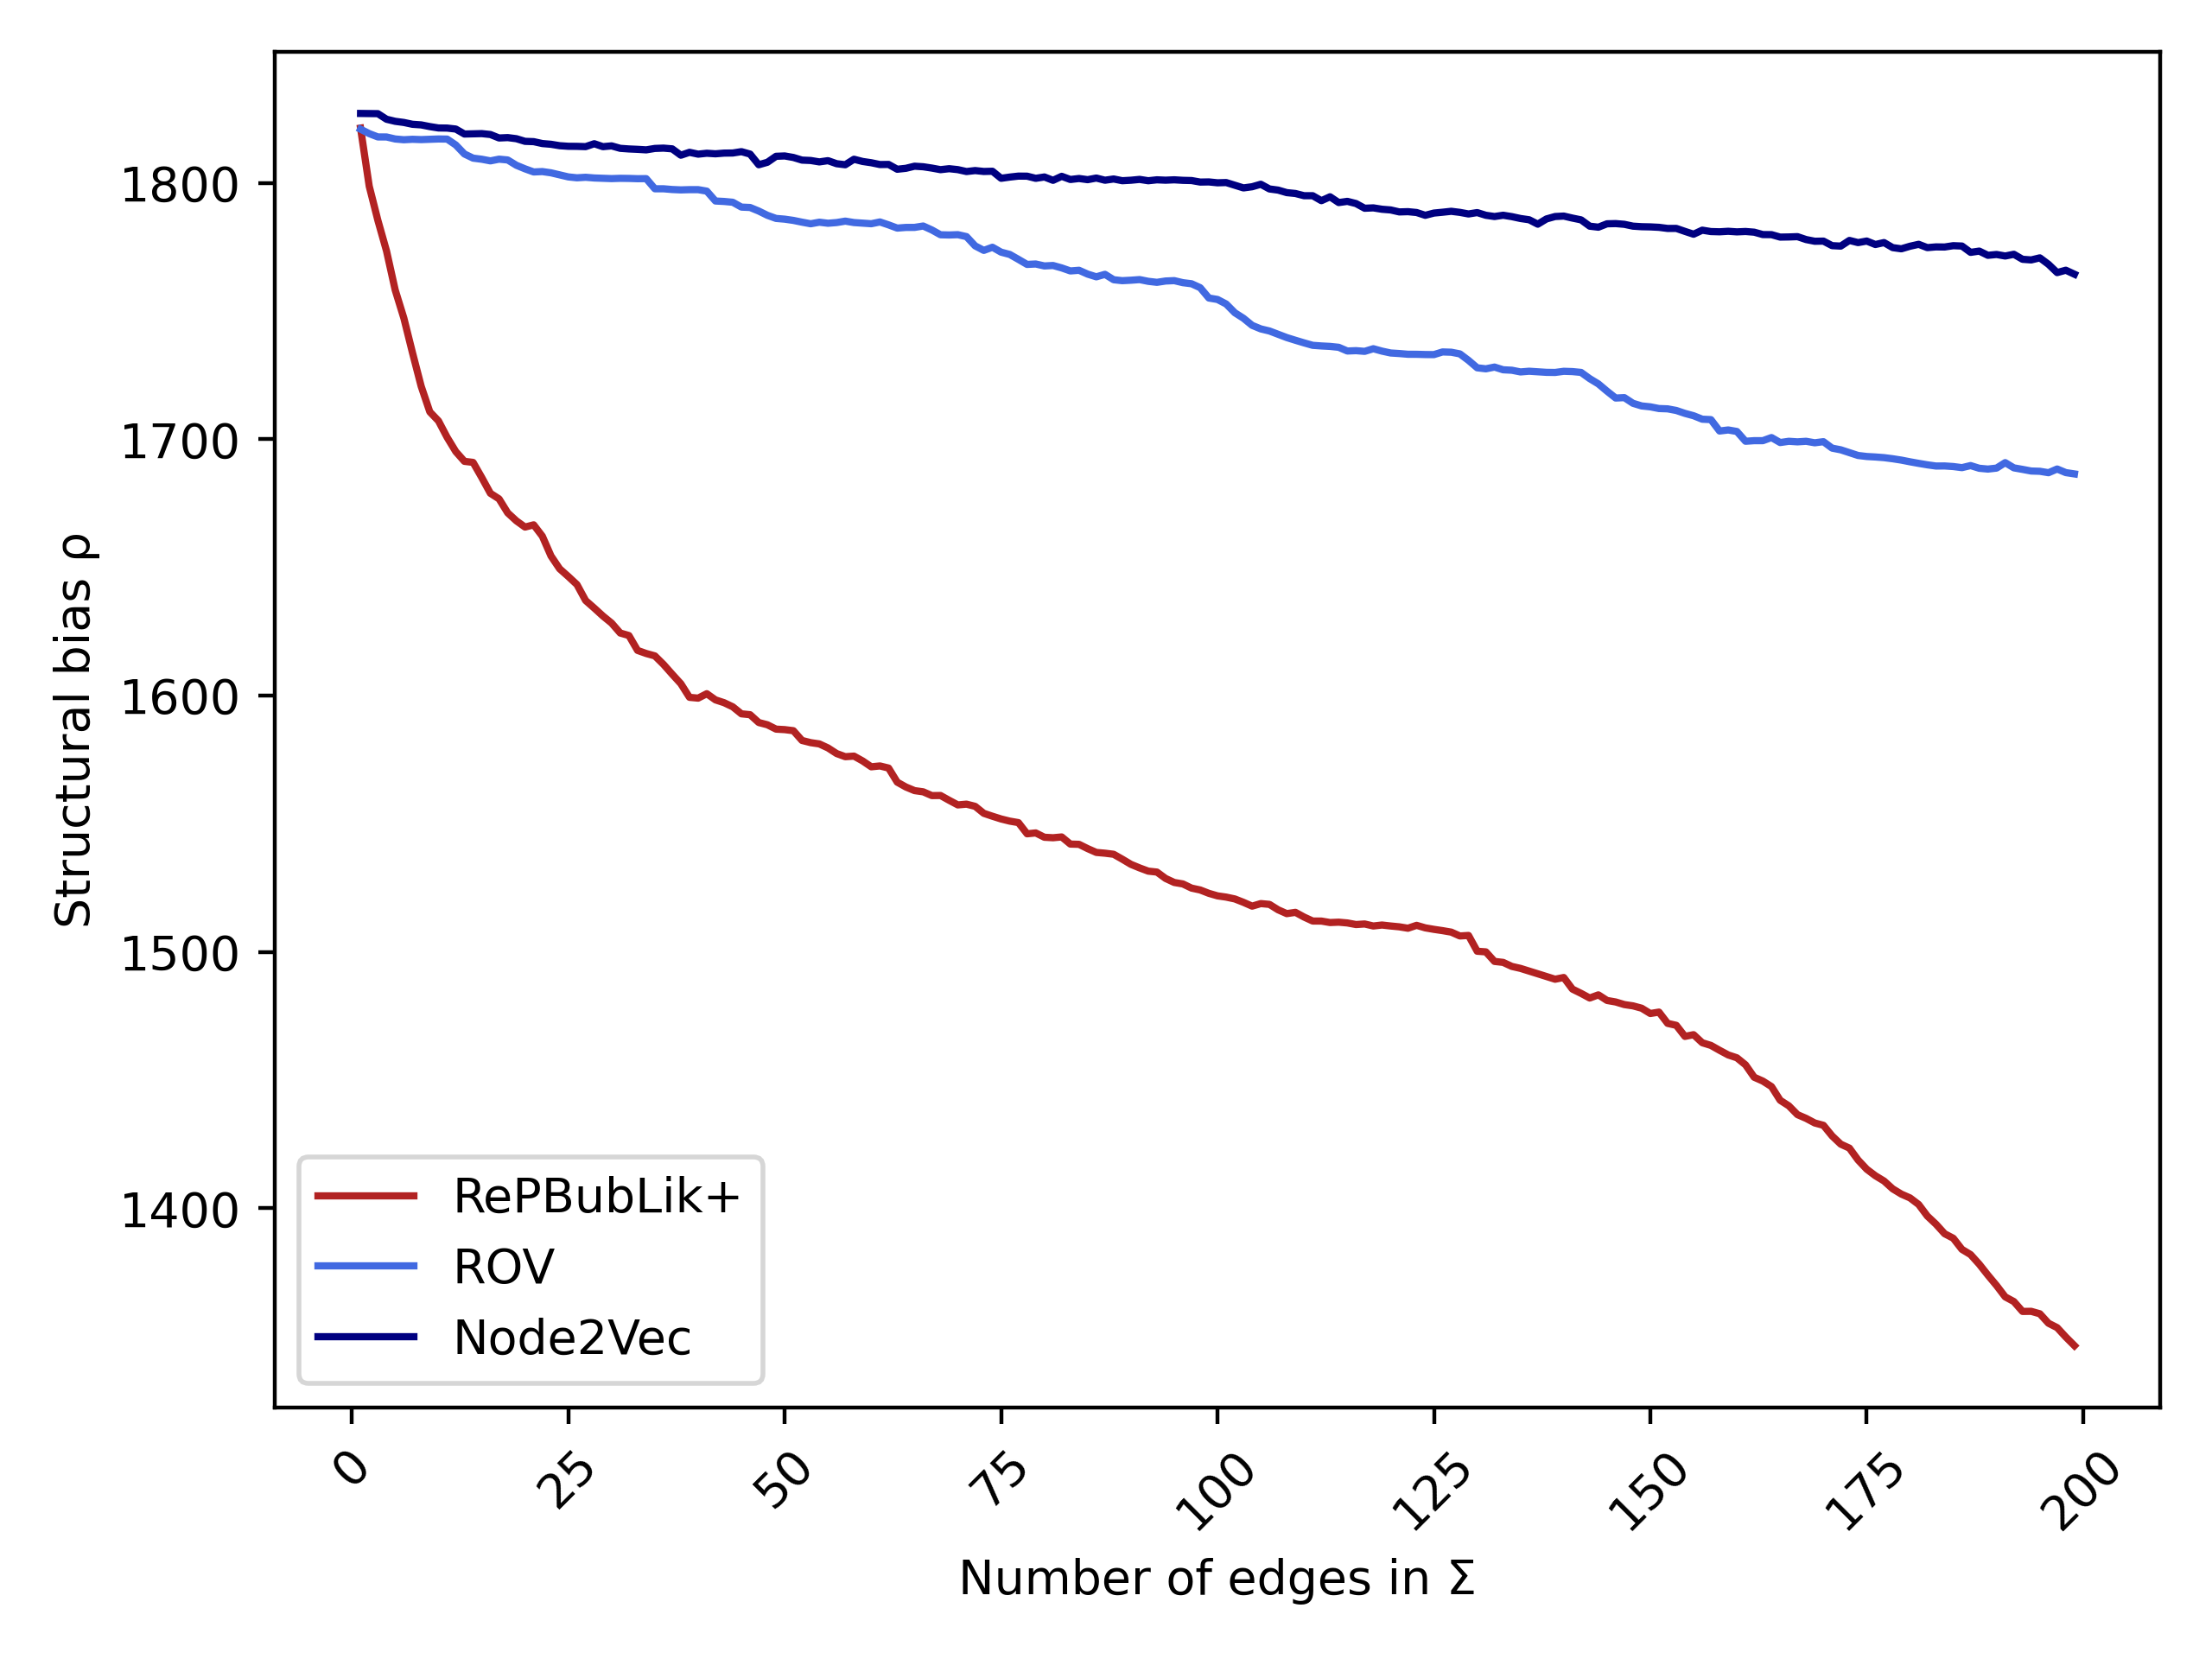
\includegraphics[width=\columnwidth]{5/polblogs_bias_5.png}
    \caption{\emph{PolBlogs} plot}\label{fig:polblogs_b_5}
\end{subfigure}
\caption{Grafici $\rho(G)$ per $t=5$}
\end{figure}
\begin{figure}[!h]
    \centering
\begin{subfigure}[b]{0.4\textwidth}
    \centering
    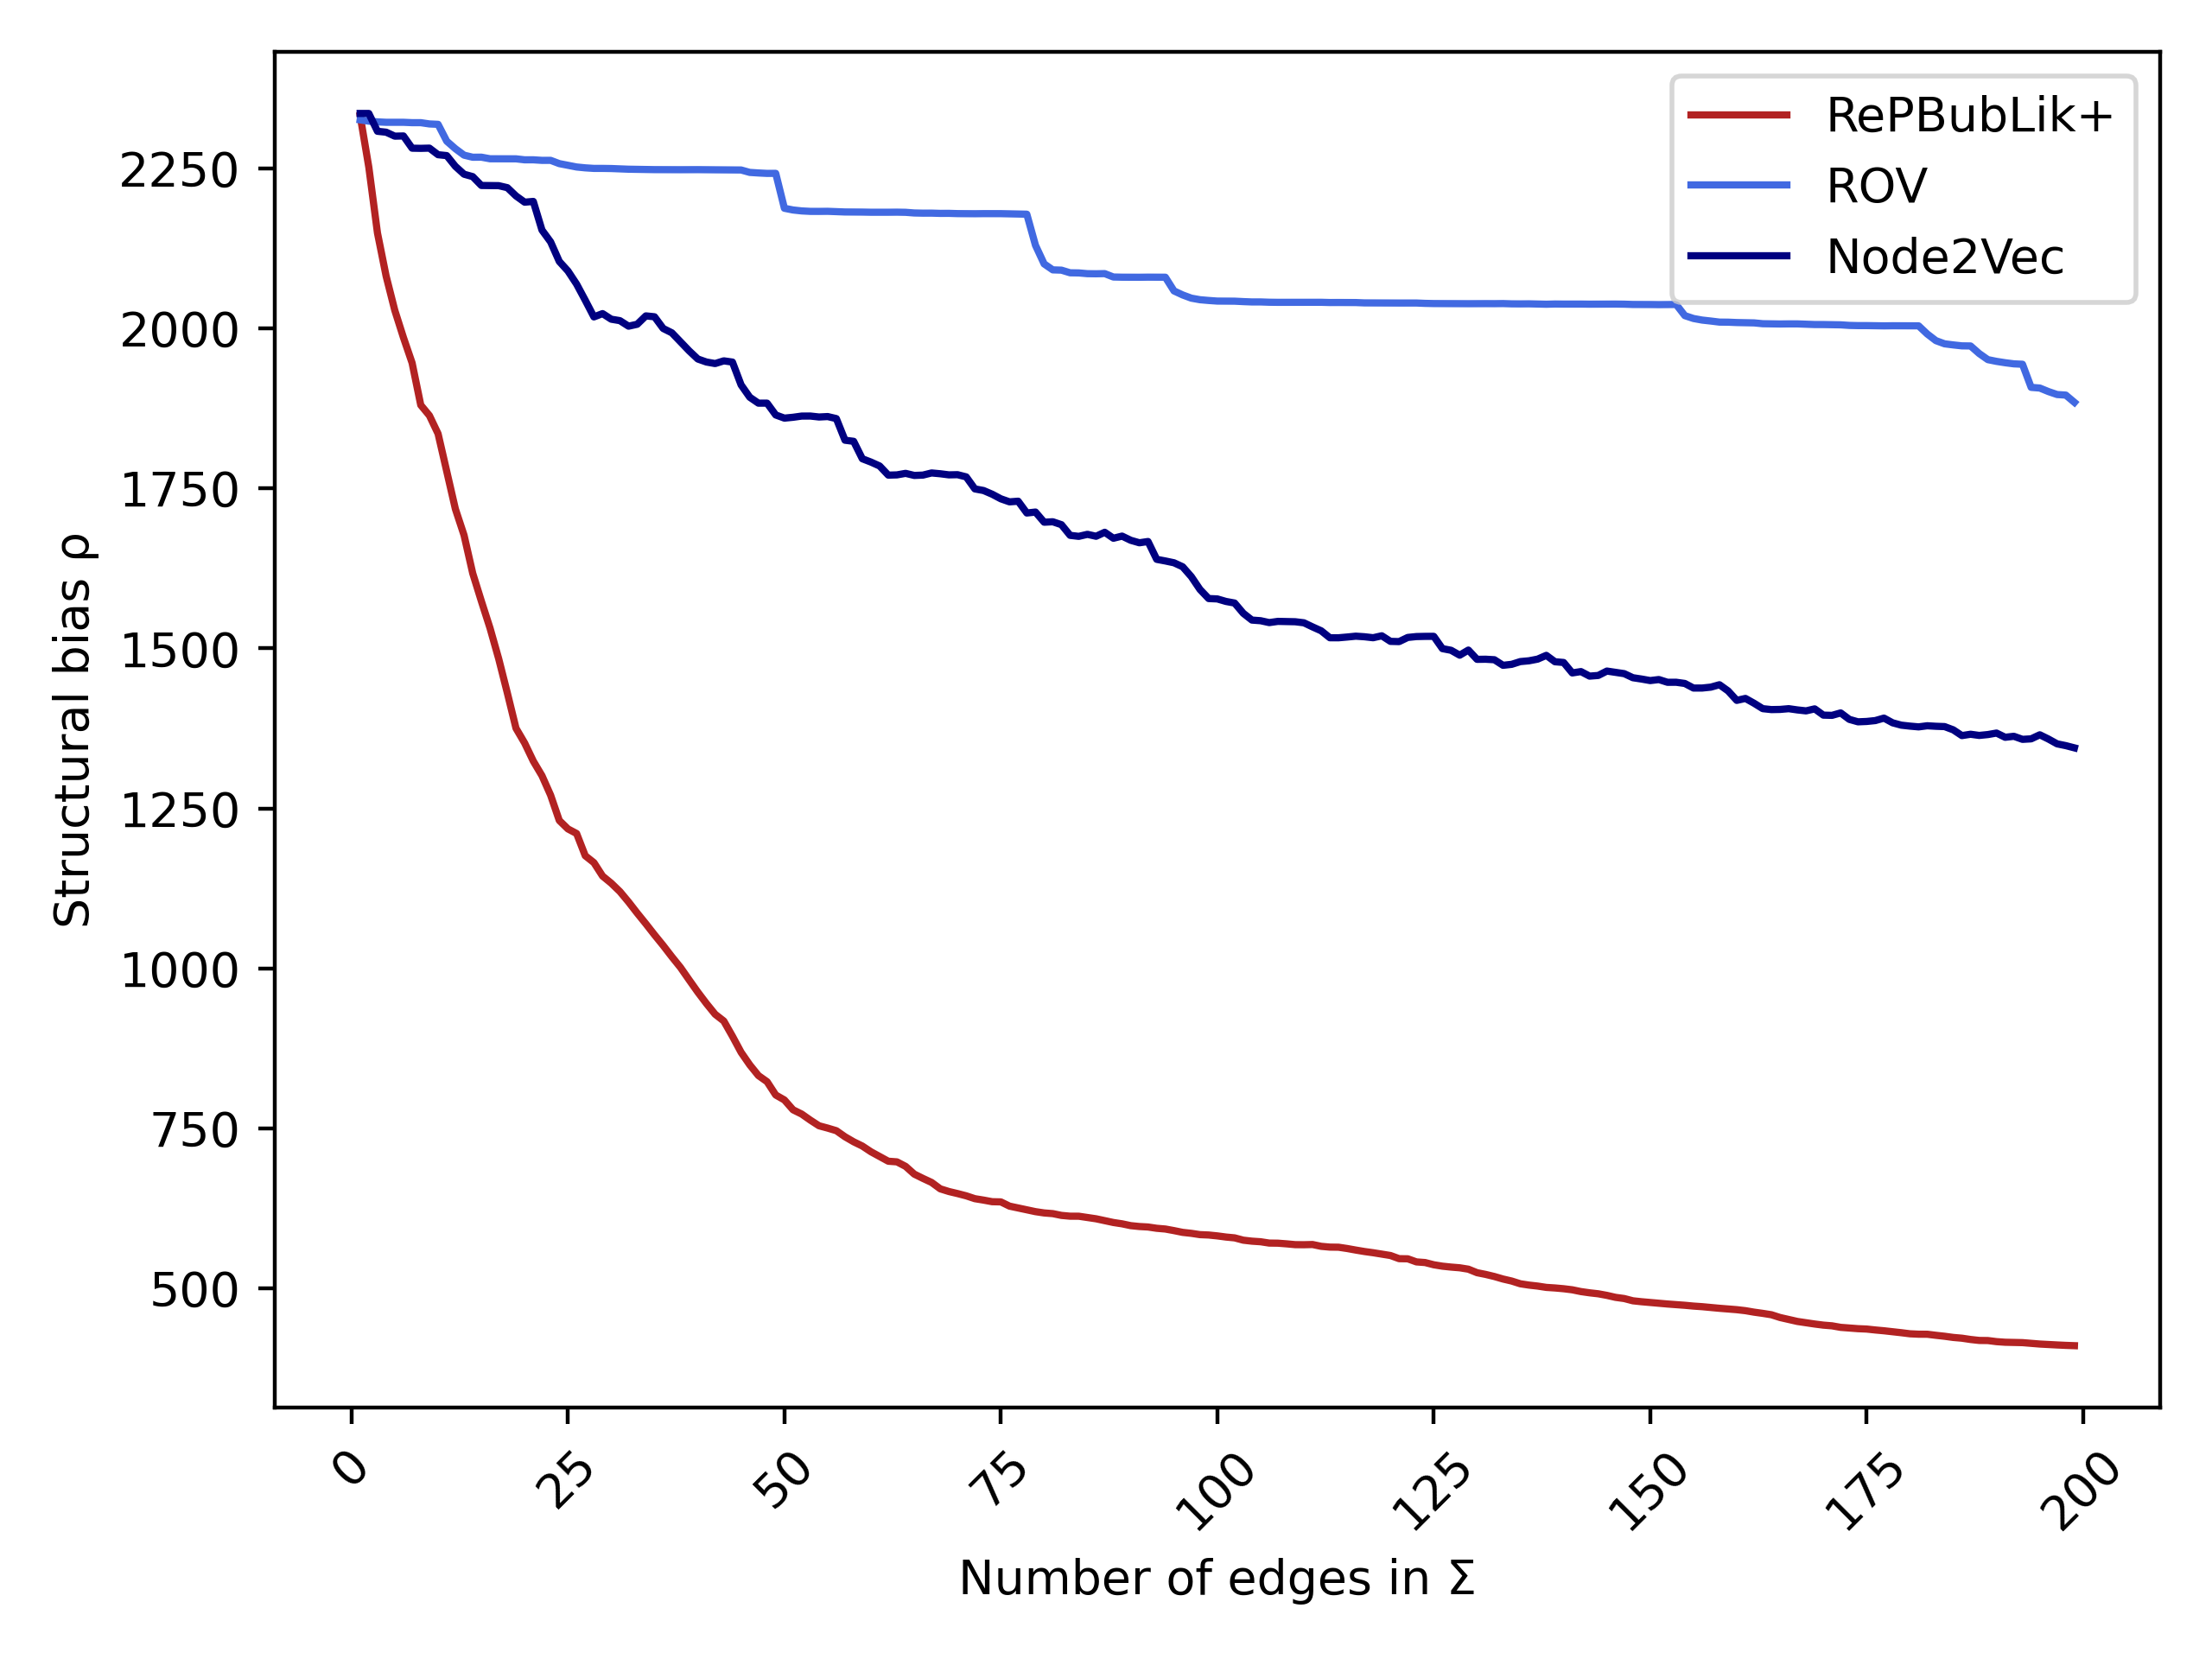
\includegraphics[width=\columnwidth]{10/math_tech_bias_10.png}
    \caption{\emph{MaTe} plot}\label{fig:mate_b_10}
\end{subfigure}
\hspace{0.1\columnwidth}
\begin{subfigure}[b]{0.4\textwidth}
    \centering
    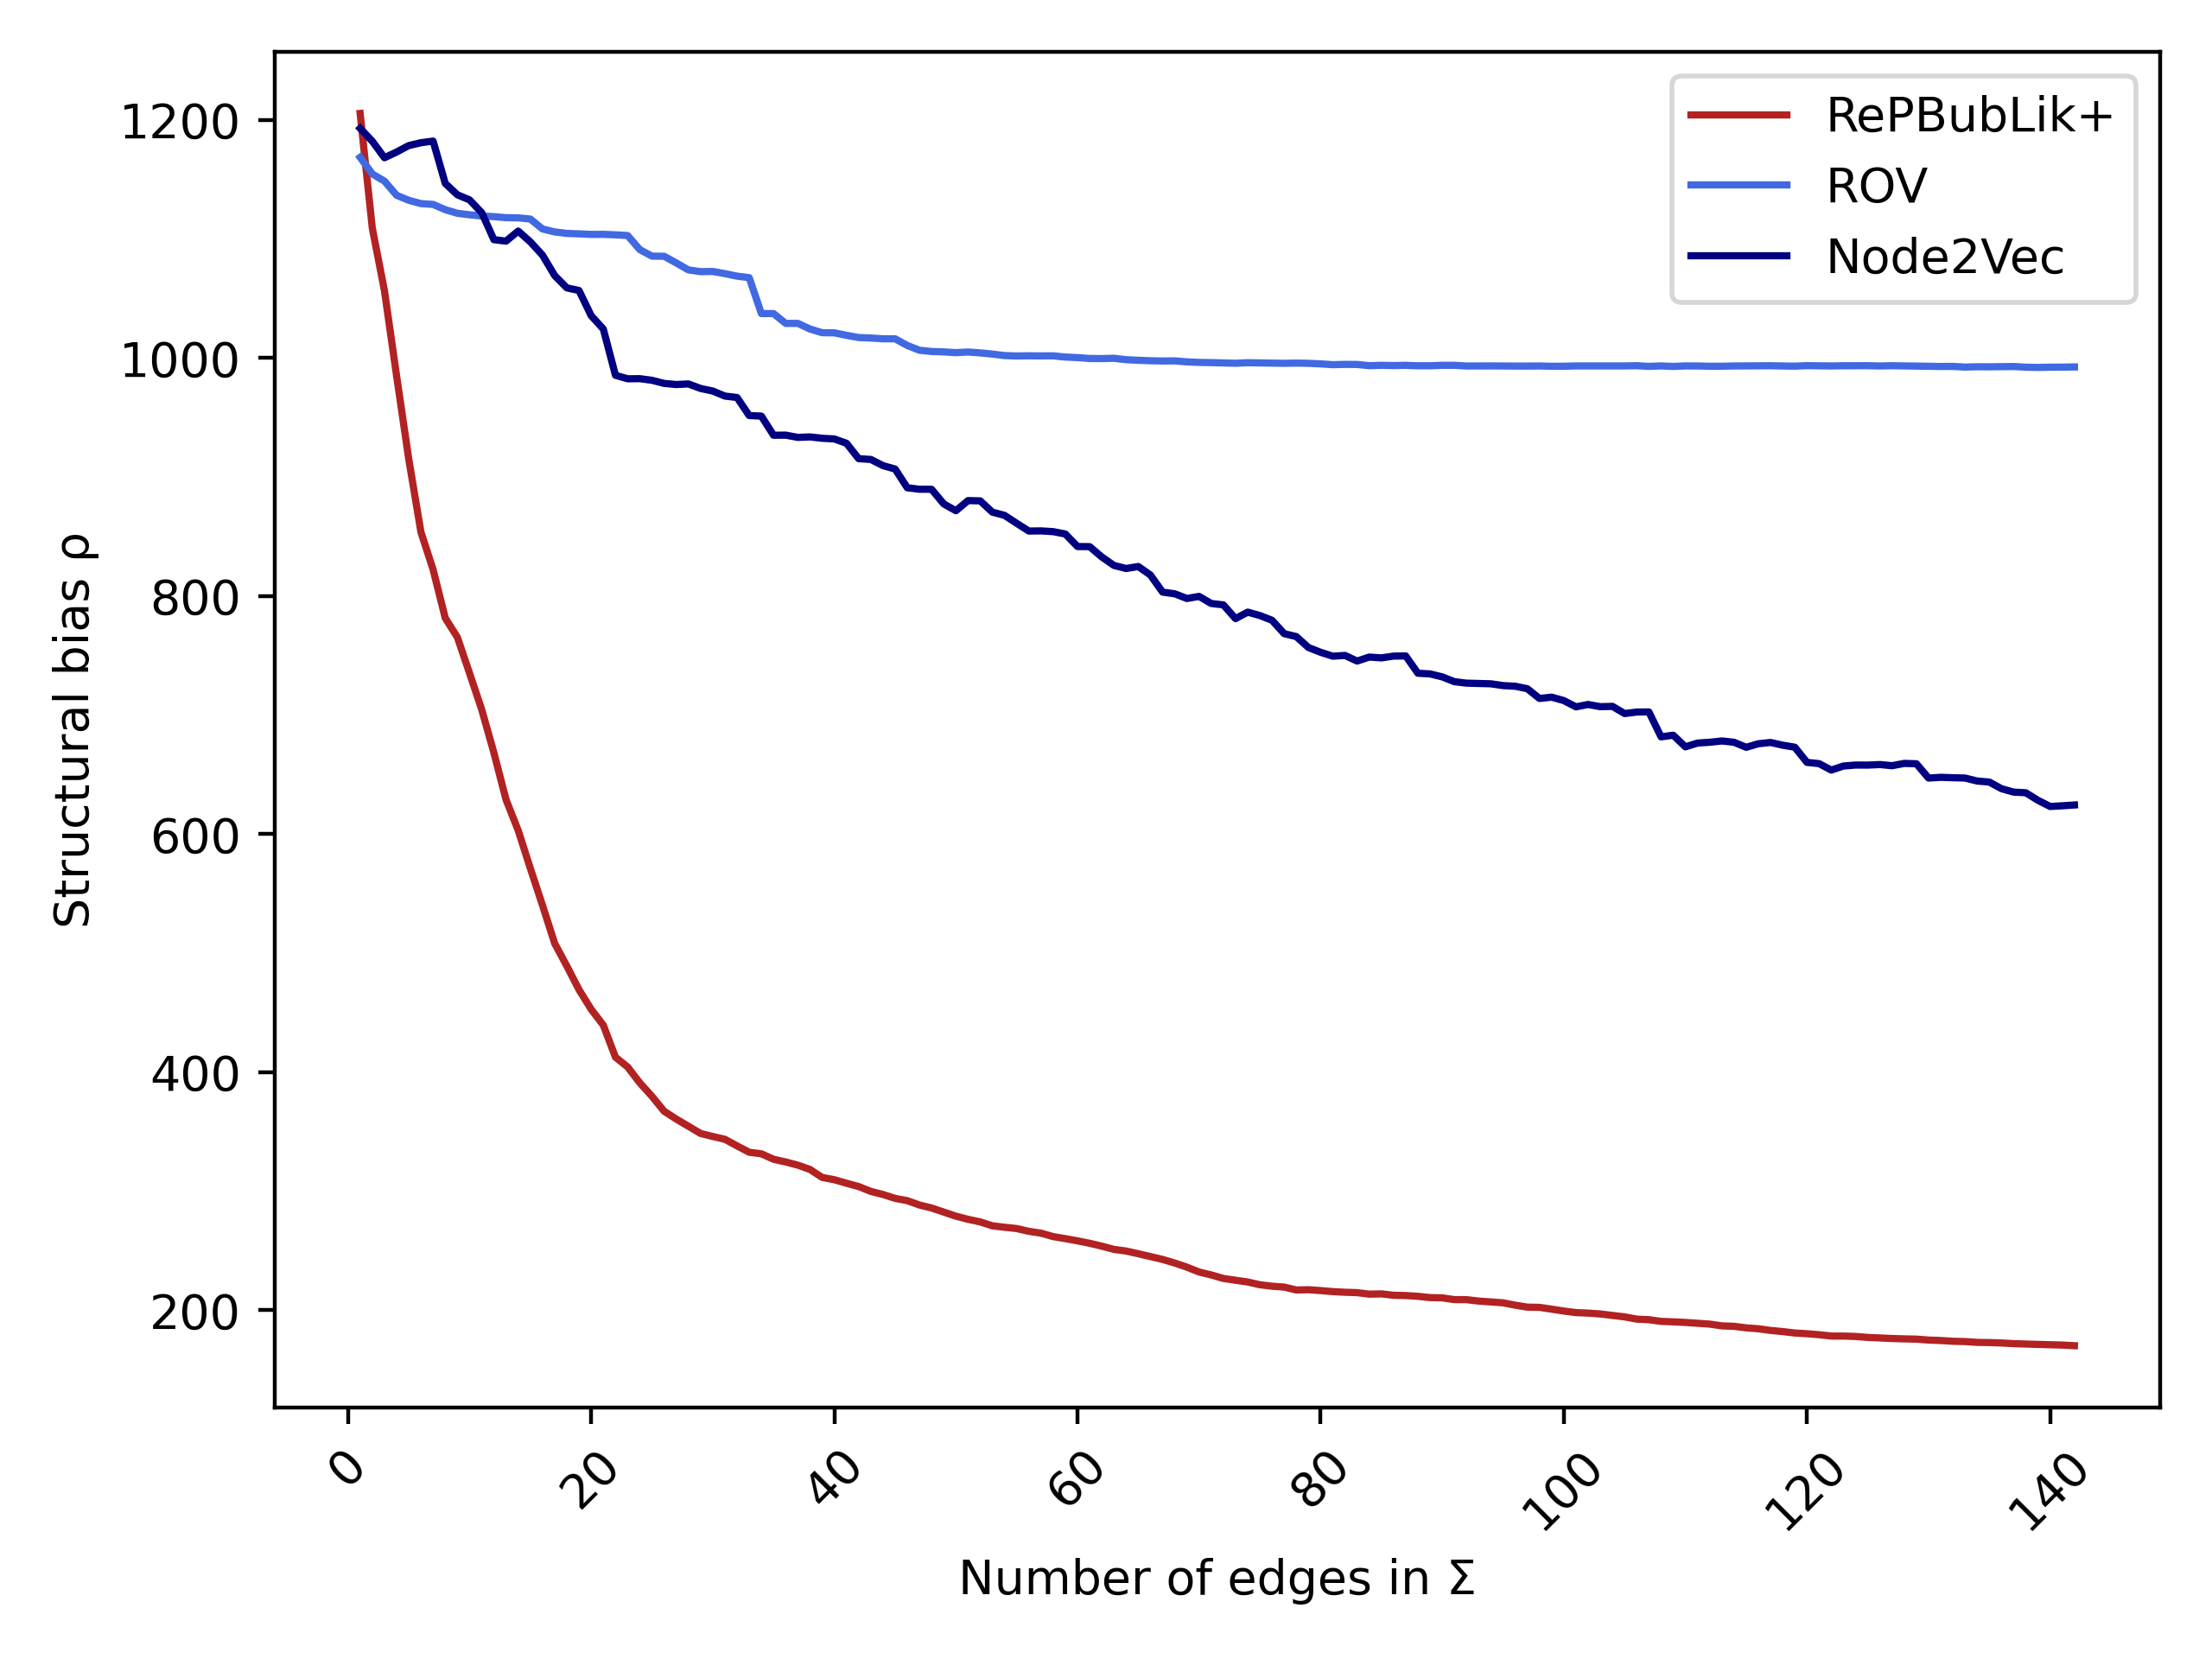
\includegraphics[width=\columnwidth]{10/tech_mil_bias_10.png}
    \caption{\emph{MiHi} plot}\label{fig:mihi_b_10}
\end{subfigure}
\end{figure}
\begin{figure}
    \ContinuedFloat
    \centering
\begin{subfigure}[b]{0.4\textwidth}
    \centering
    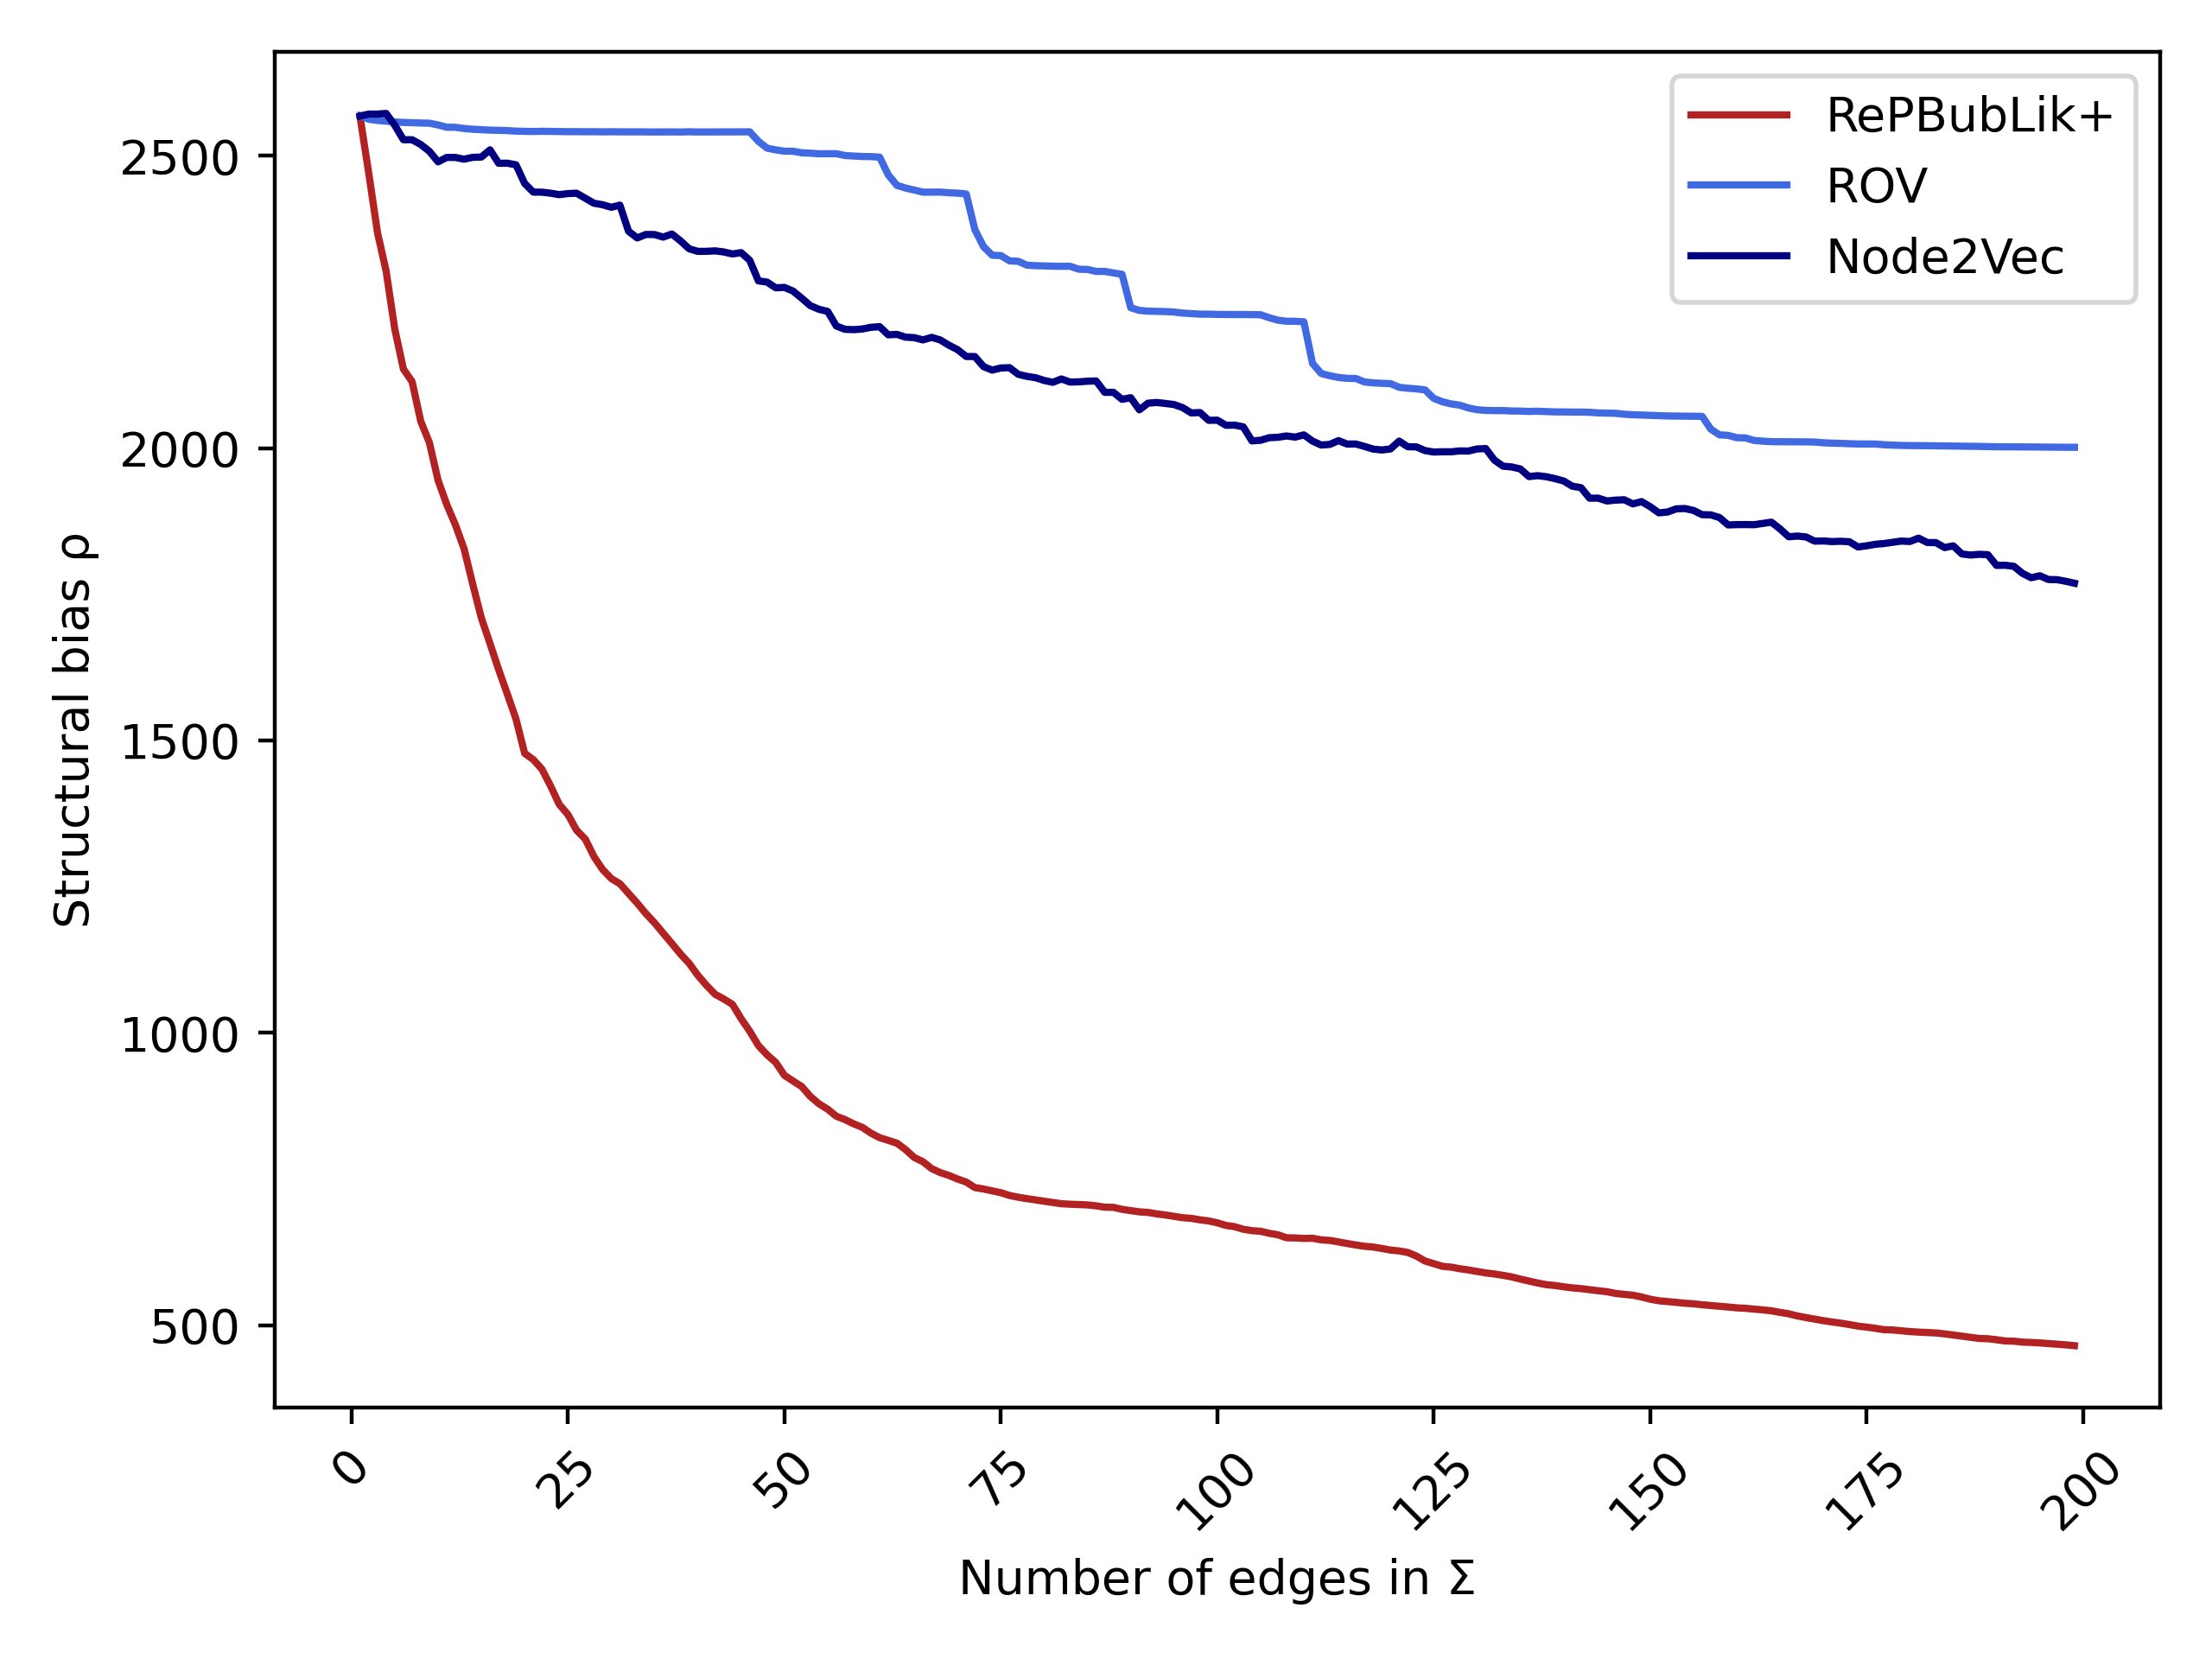
\includegraphics[width=\columnwidth]{10/math_ast_bias_10.png}
    \caption{\emph{MaA}s plot}\label{fig:maas_b_10}
\end{subfigure}
\hspace{0.1\columnwidth}
\begin{subfigure}[b]{0.4\textwidth}
    \centering
    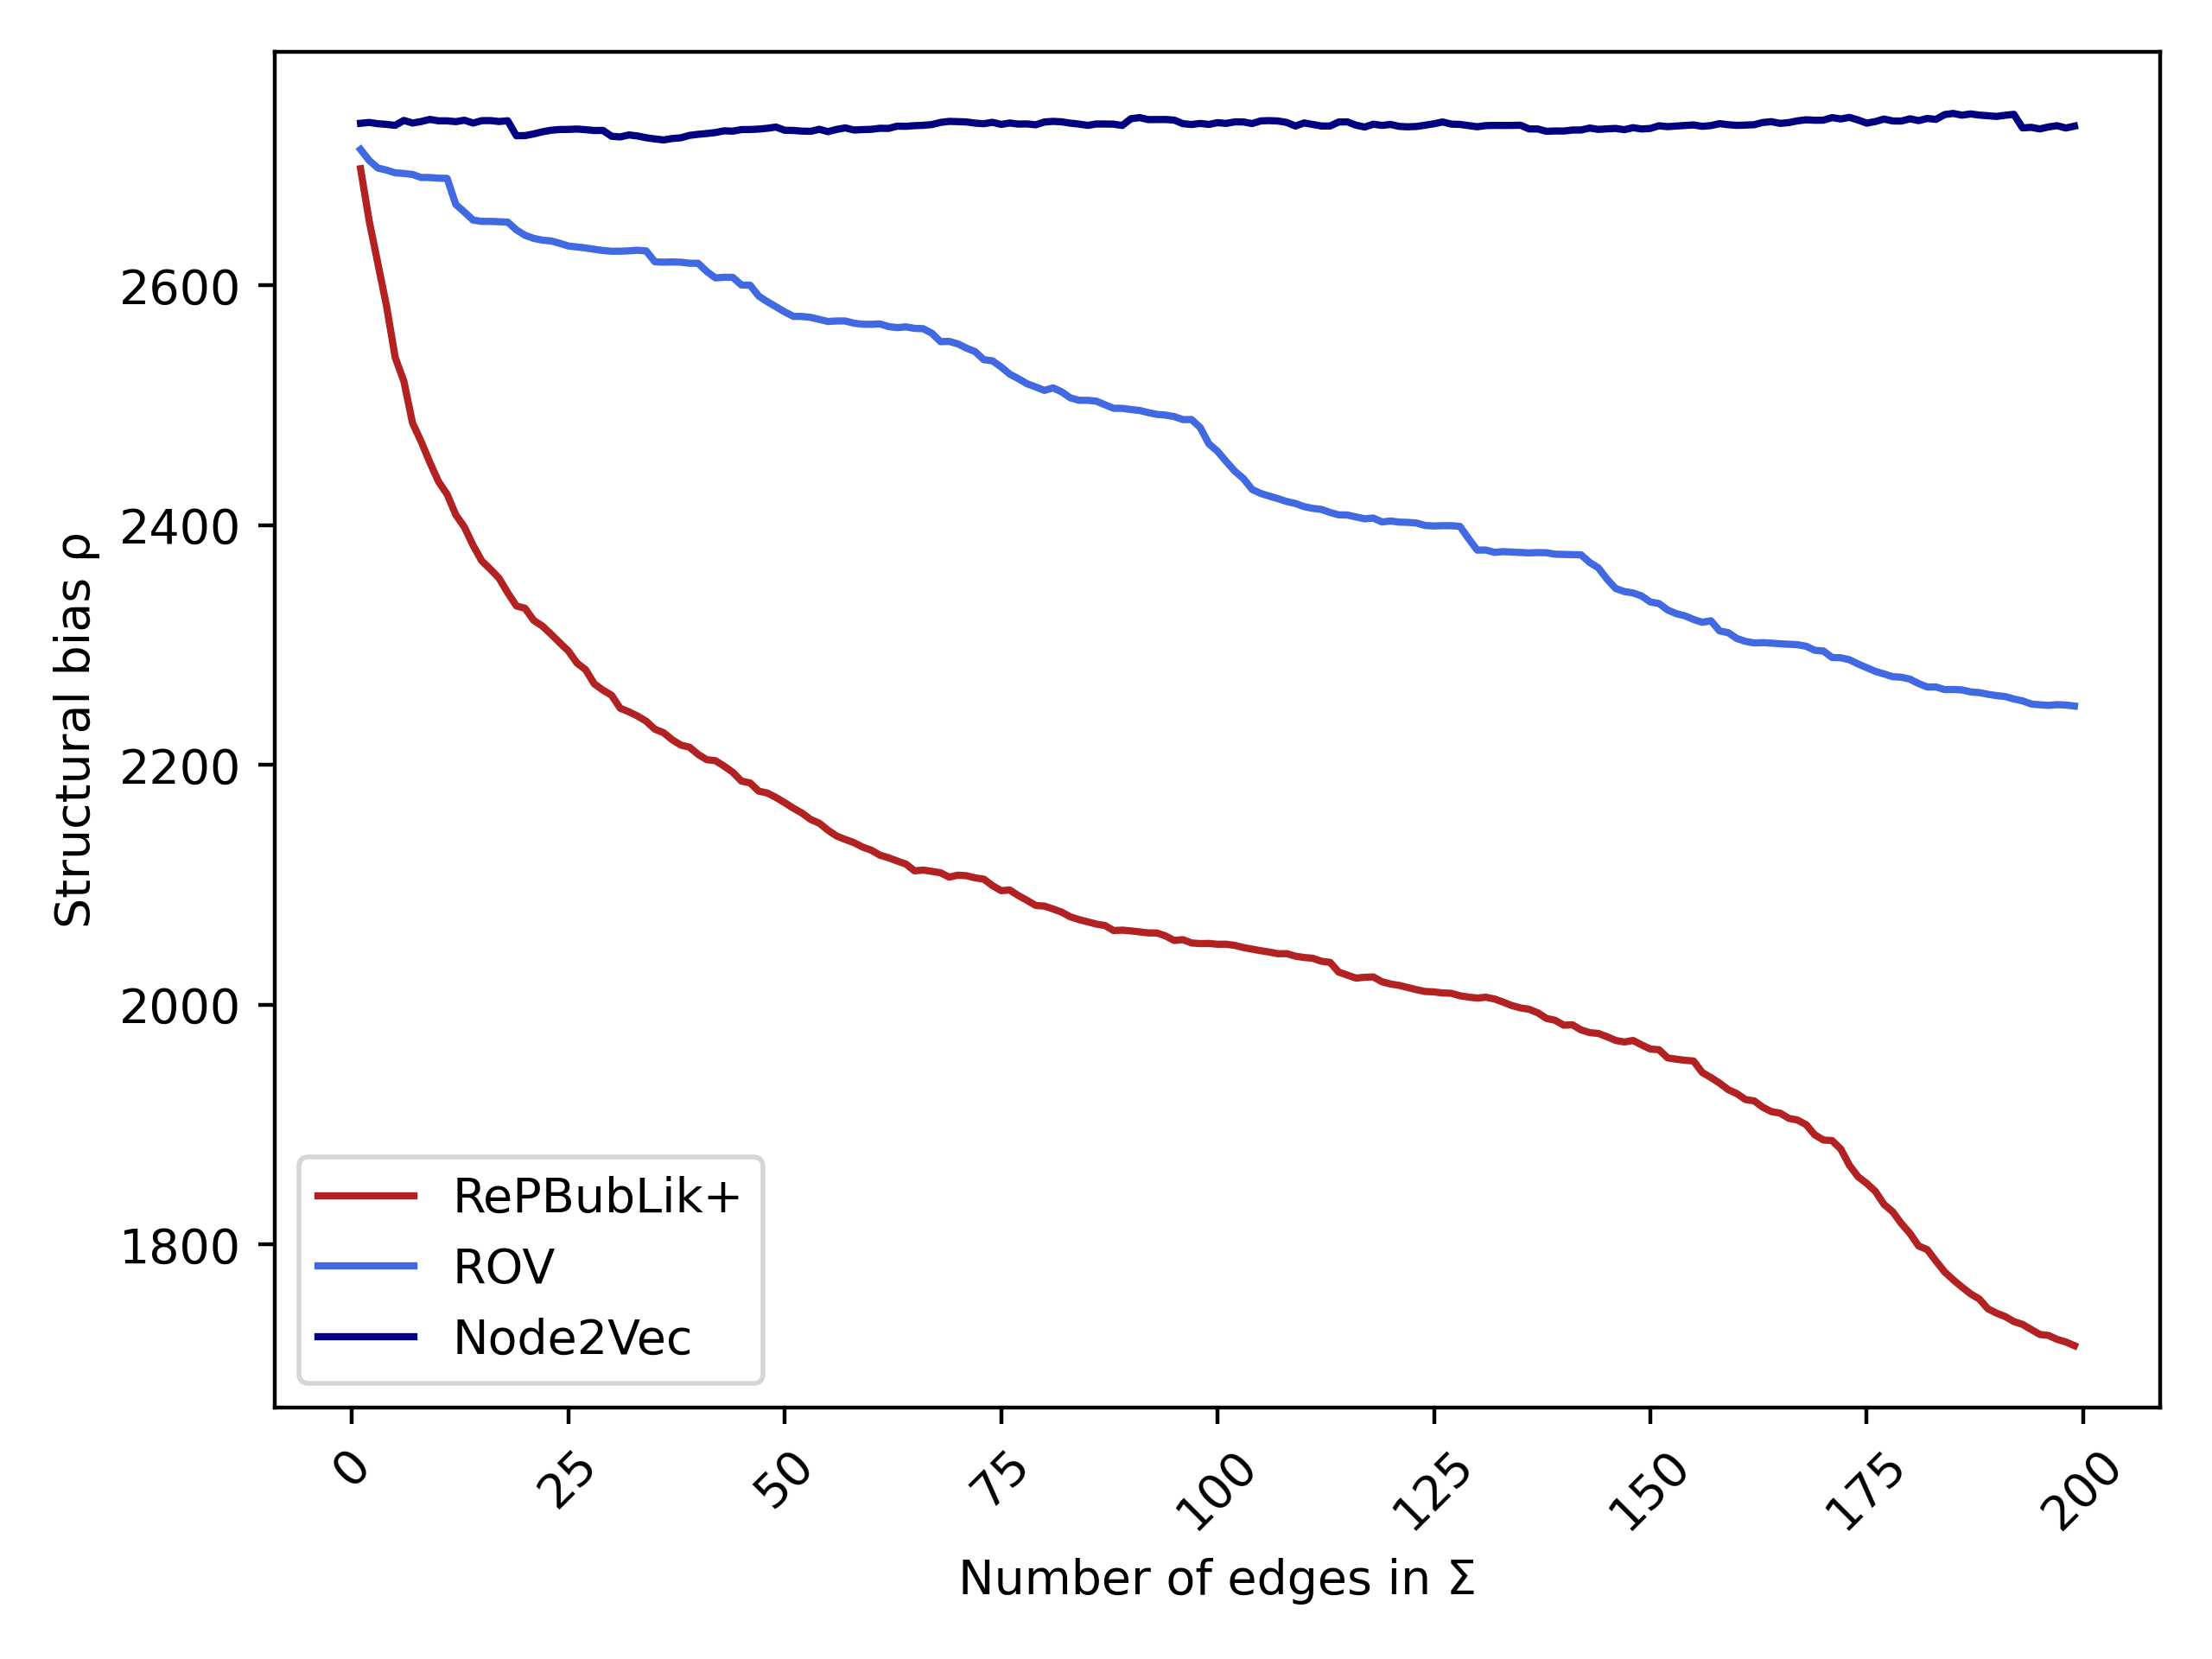
\includegraphics[width=\columnwidth]{10/polblogs_bias_10.png}
    \caption{\emph{PolBlogs} plot}\label{fig:polblogs_b_10}
\end{subfigure}
\caption{Grafici $\rho(G)$ per $t=10$}
\end{figure}
\newpage
\begin{figure}[!h]
    \centering
\begin{subfigure}[b]{0.4\textwidth}
    \centering
    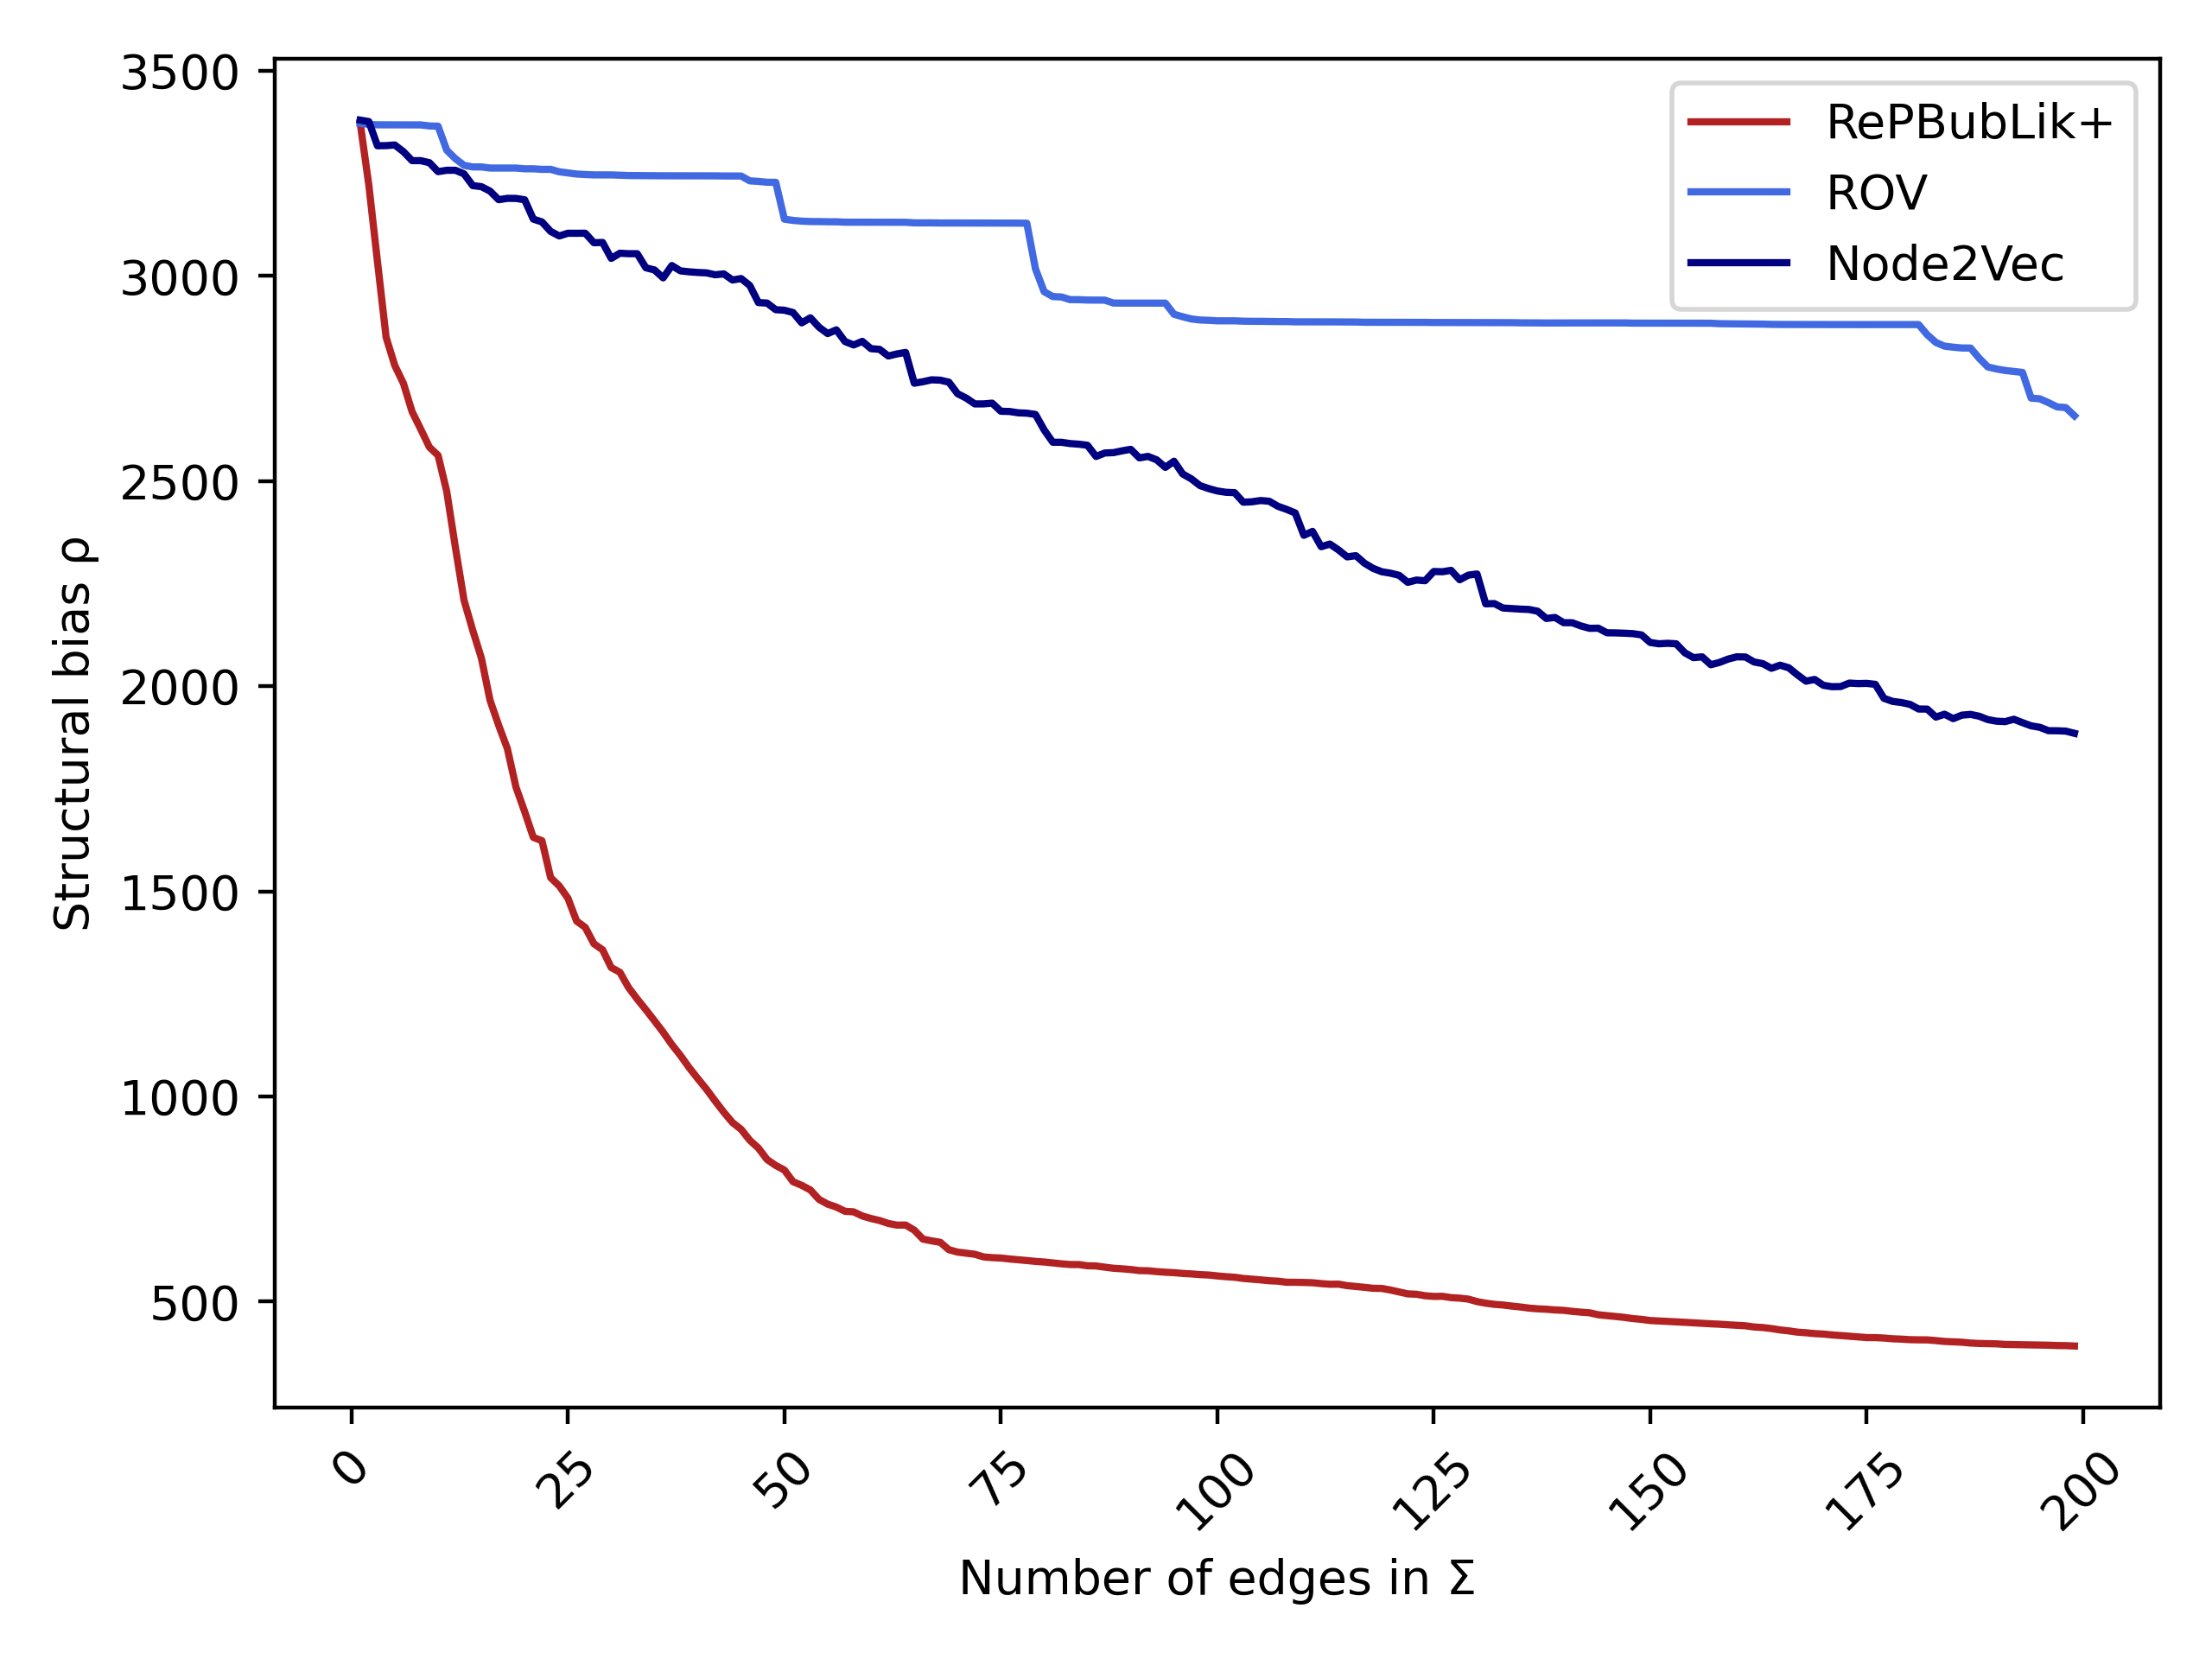
\includegraphics[width=\columnwidth]{15/math_tech_bias_15.png}
    \caption{\emph{MaTe} plot}\label{fig:mate_b_15}
\end{subfigure}
\hspace{0.1\columnwidth}
\begin{subfigure}[b]{0.4\textwidth}
    \centering
    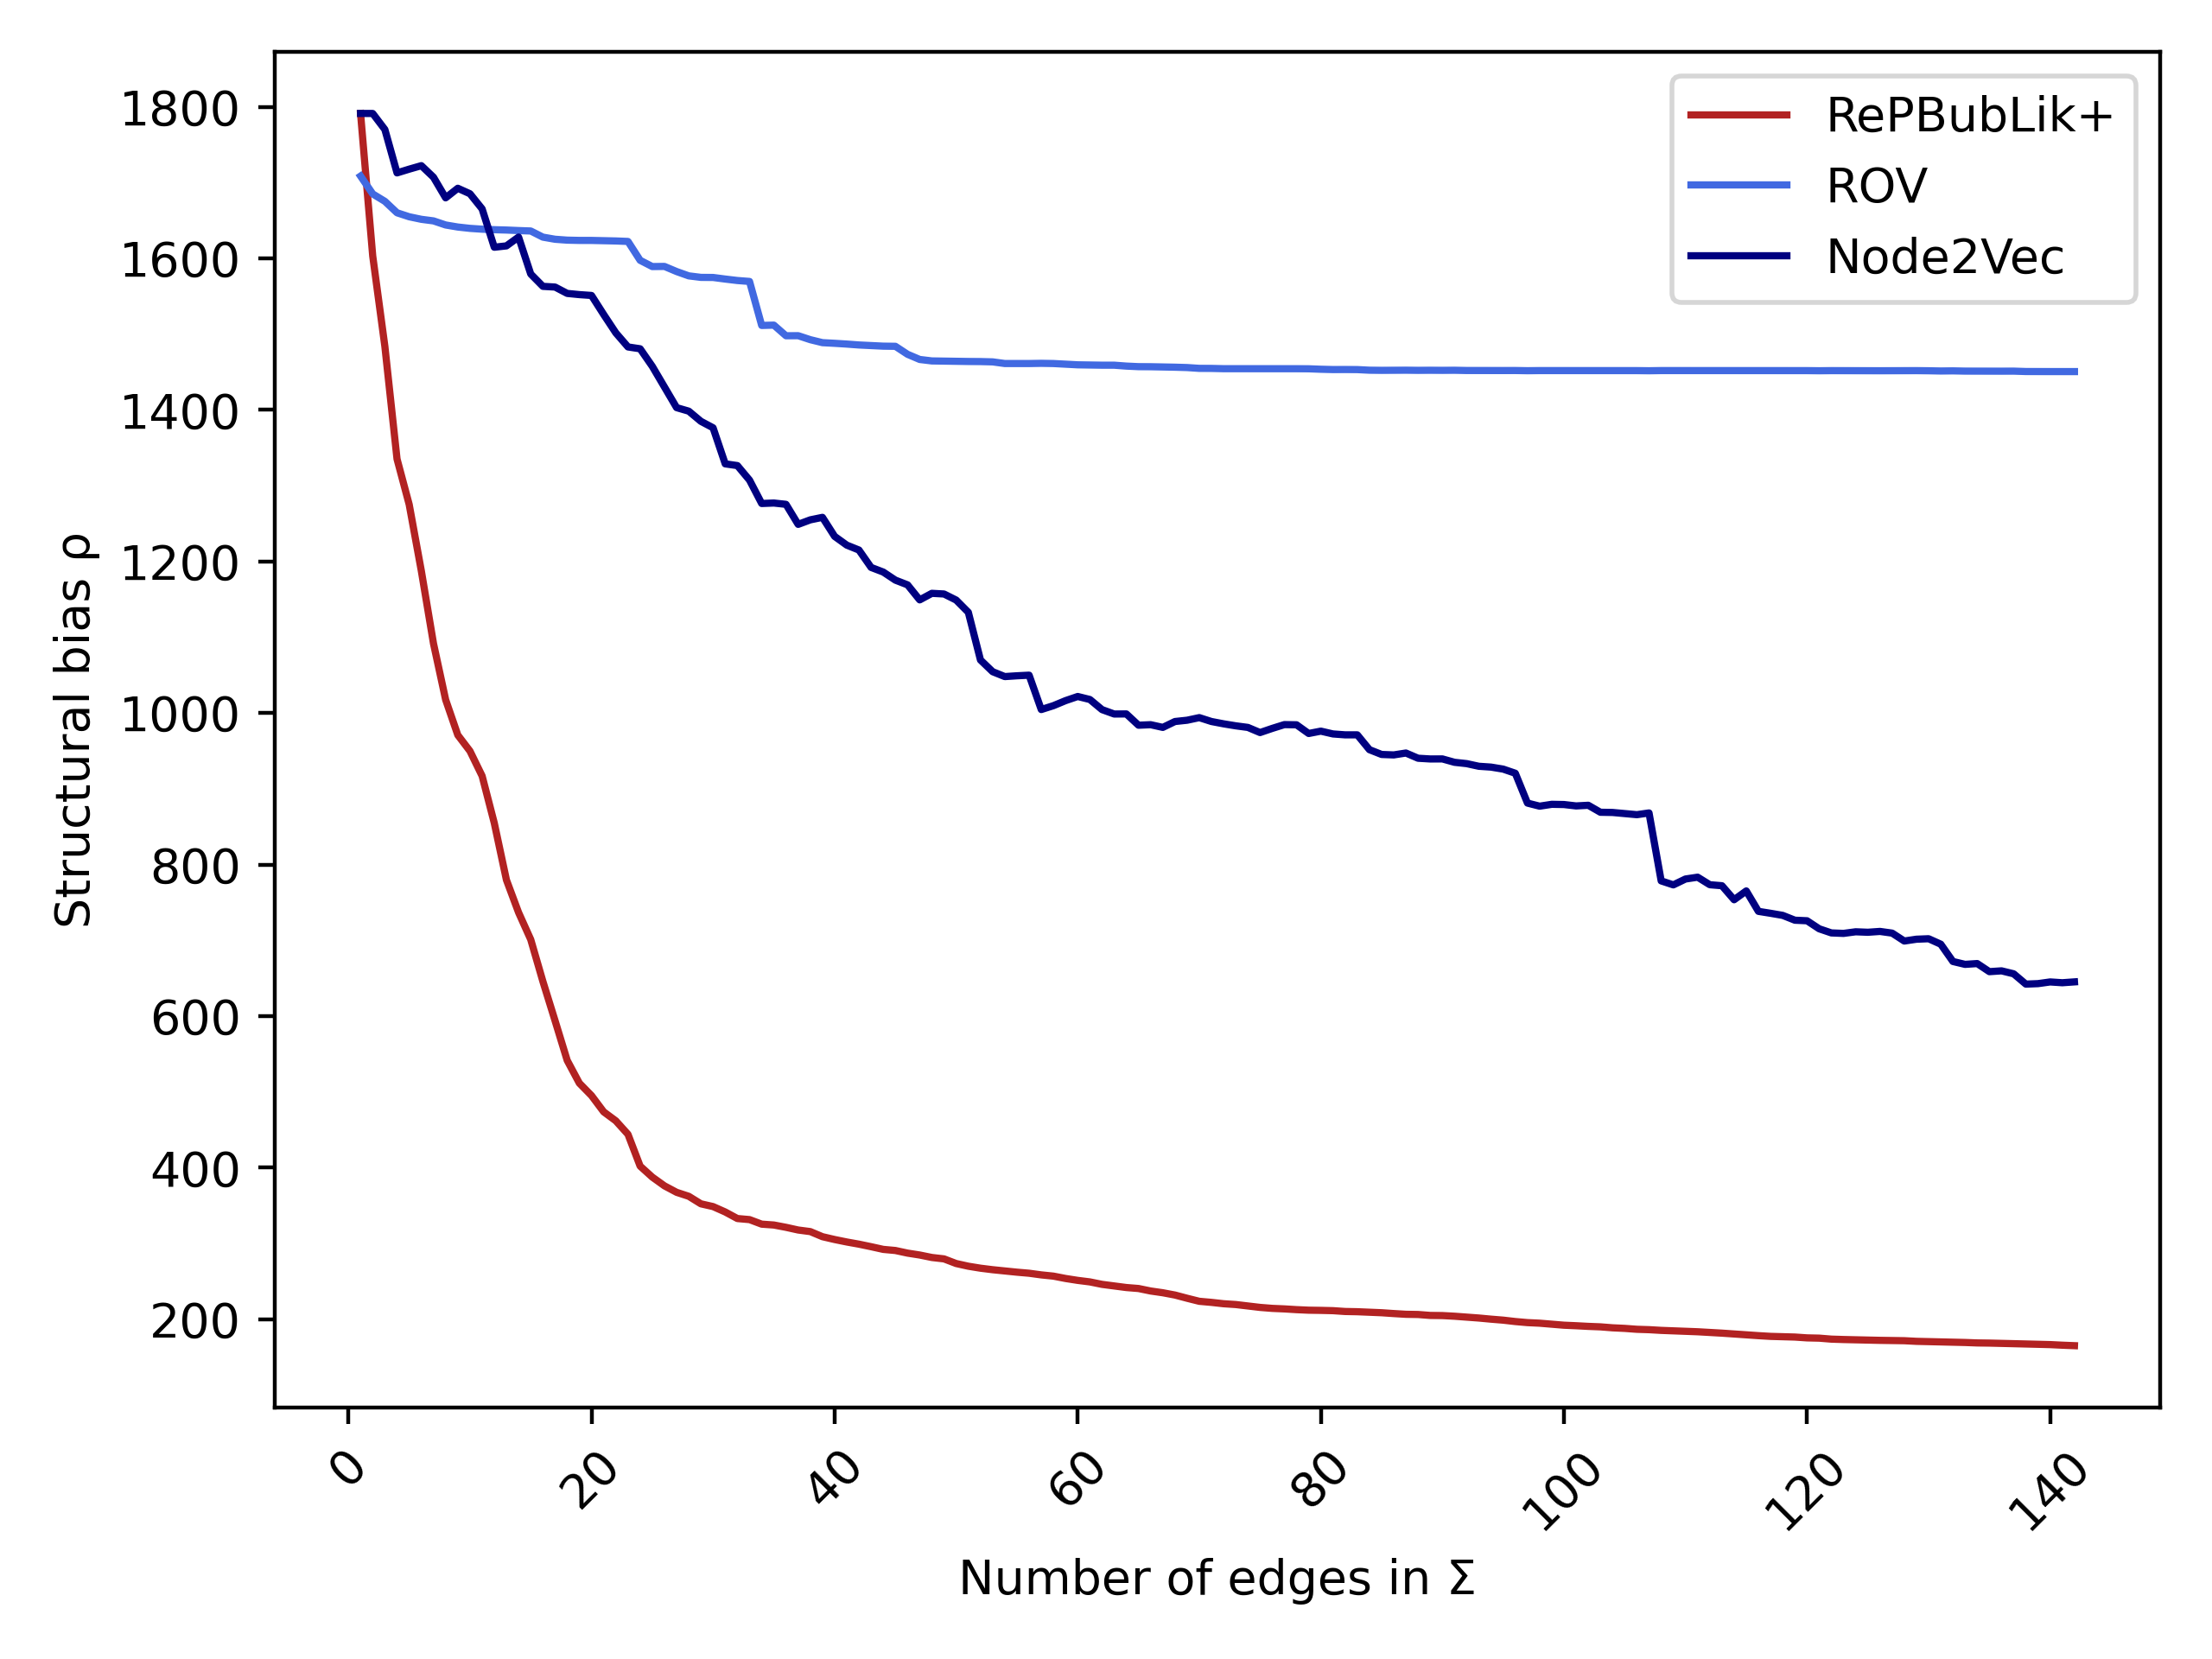
\includegraphics[width=\columnwidth]{15/tech_mil_bias_15.png}
    \caption{\emph{MiHi} plot}\label{fig:mihi_b_15}
\end{subfigure}

\begin{subfigure}[b]{0.4\textwidth}
    \centering
    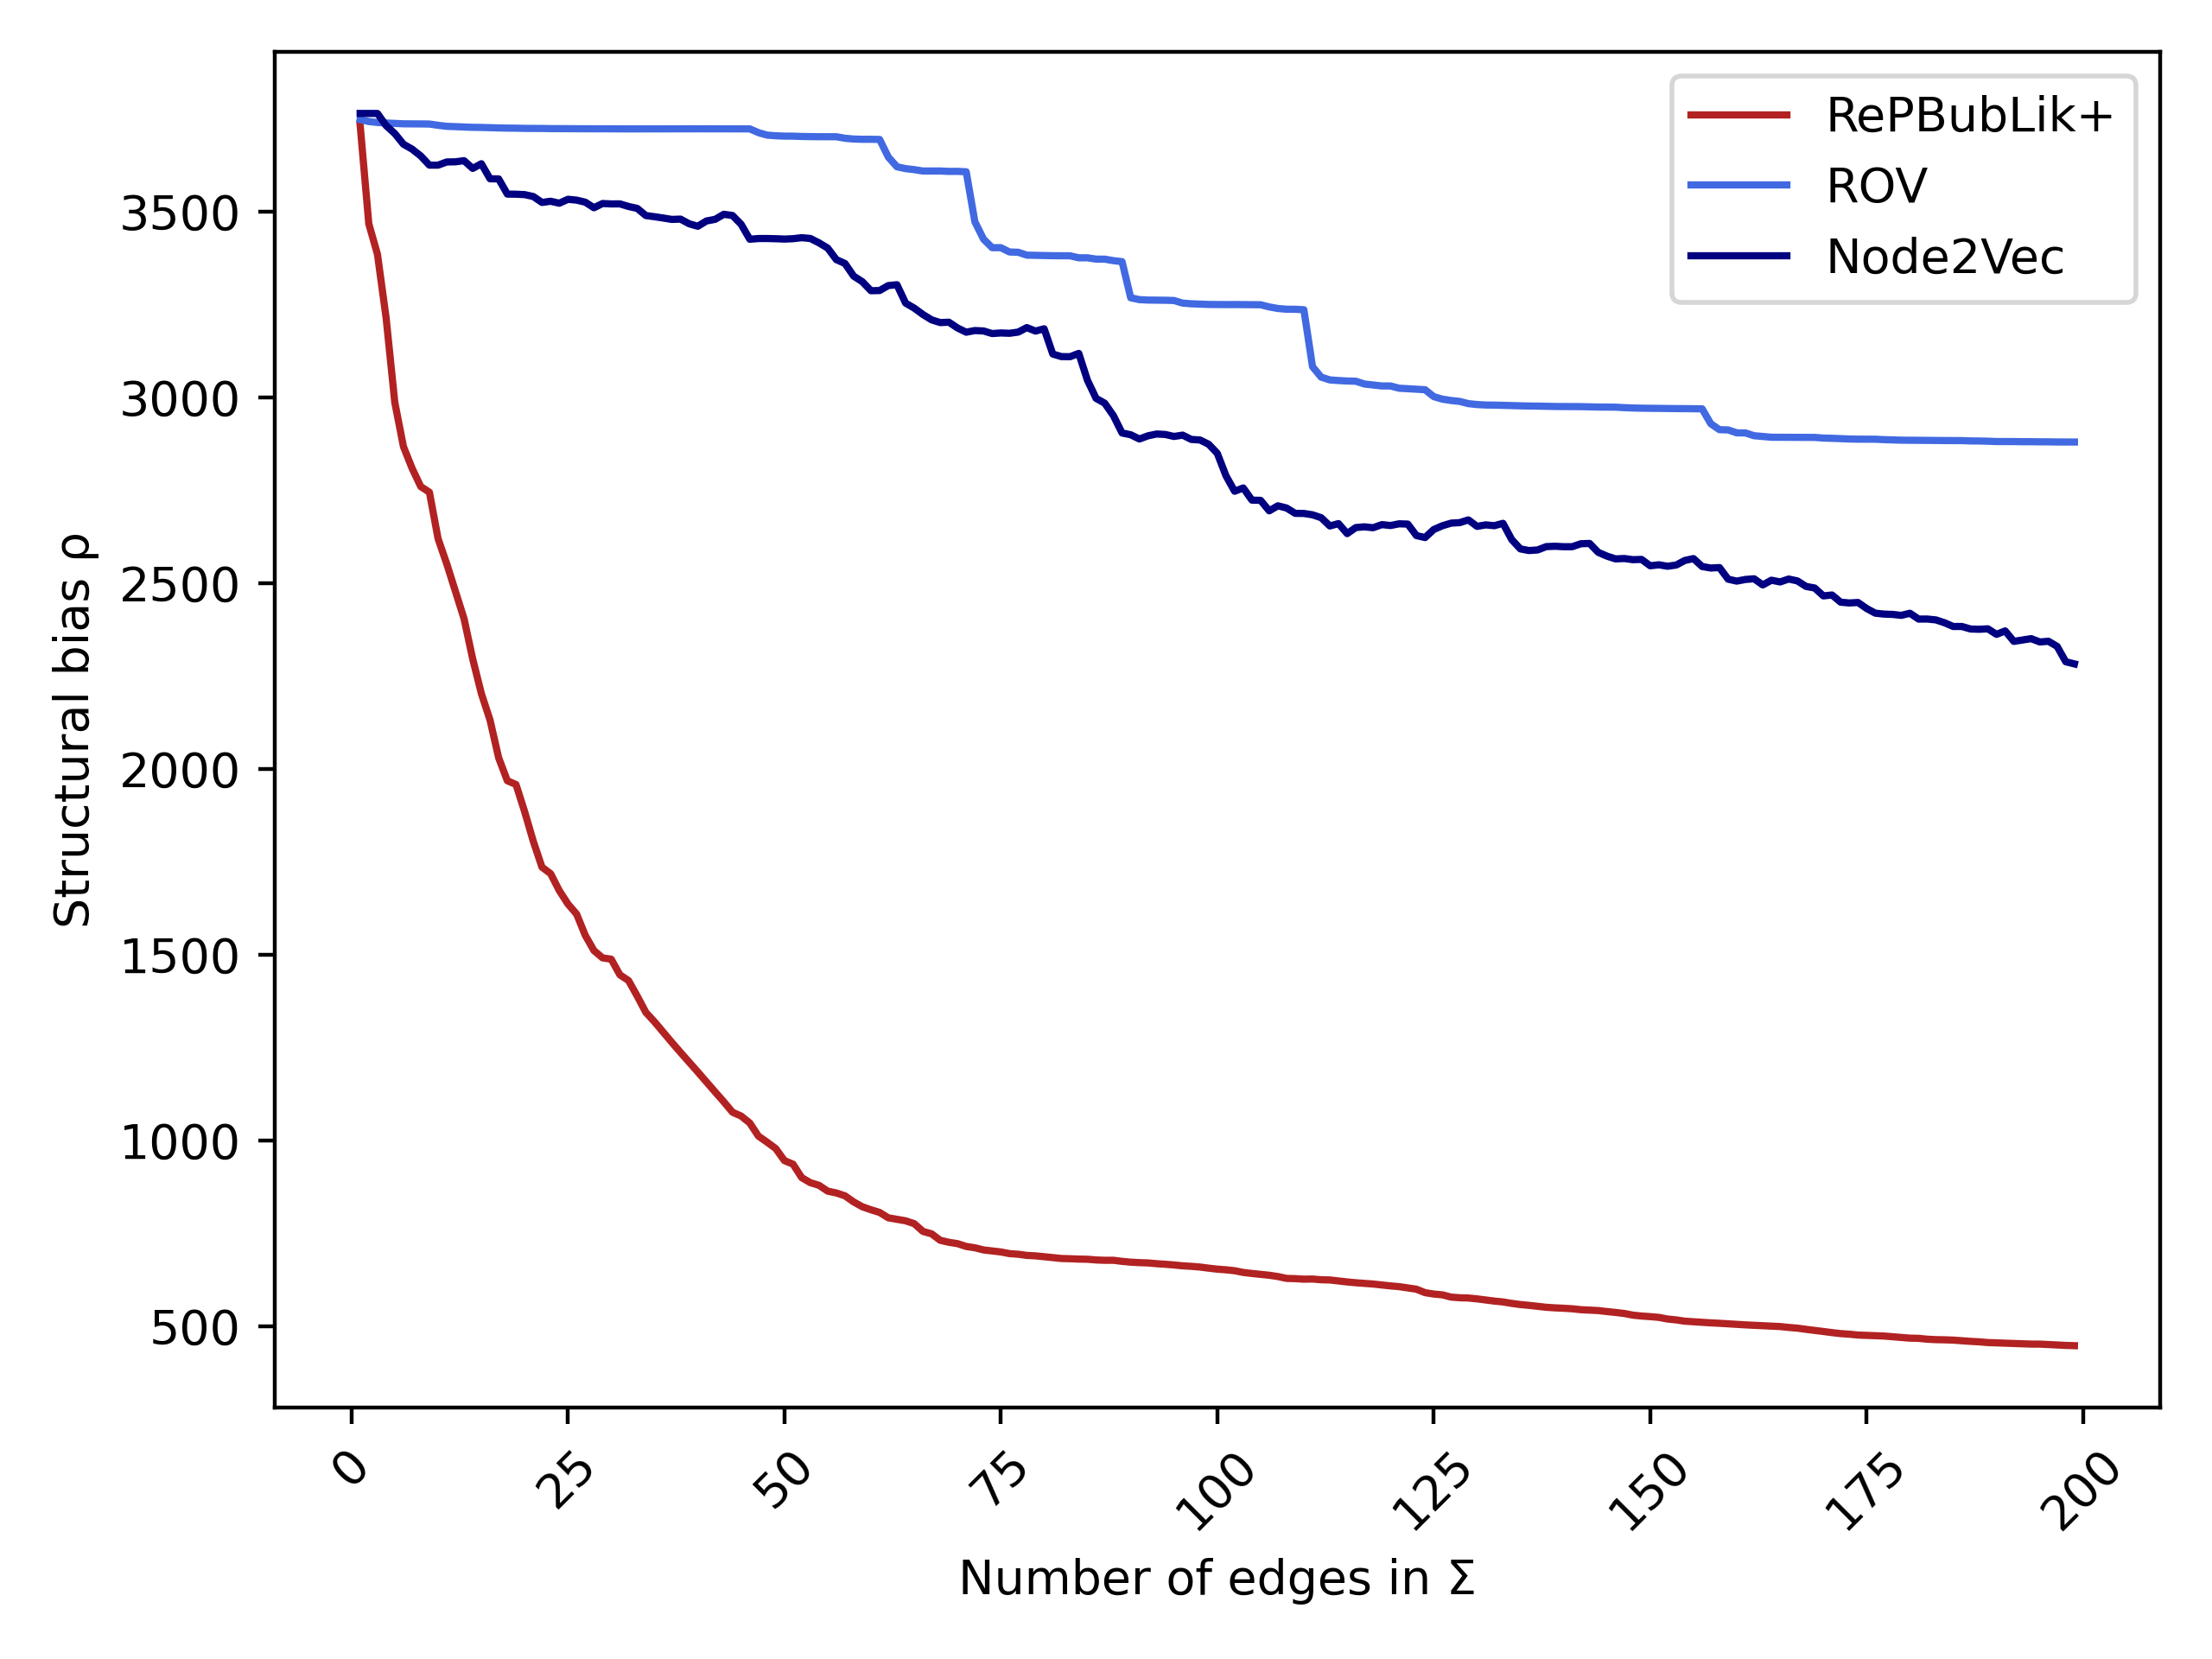
\includegraphics[width=\columnwidth]{15/math_ast_bias_15.png}
    \caption{\emph{MaA}s plot}\label{fig:maas_b_15}
\end{subfigure}
\hspace{0.1\columnwidth}
\begin{subfigure}[b]{0.4\textwidth}
    \centering
    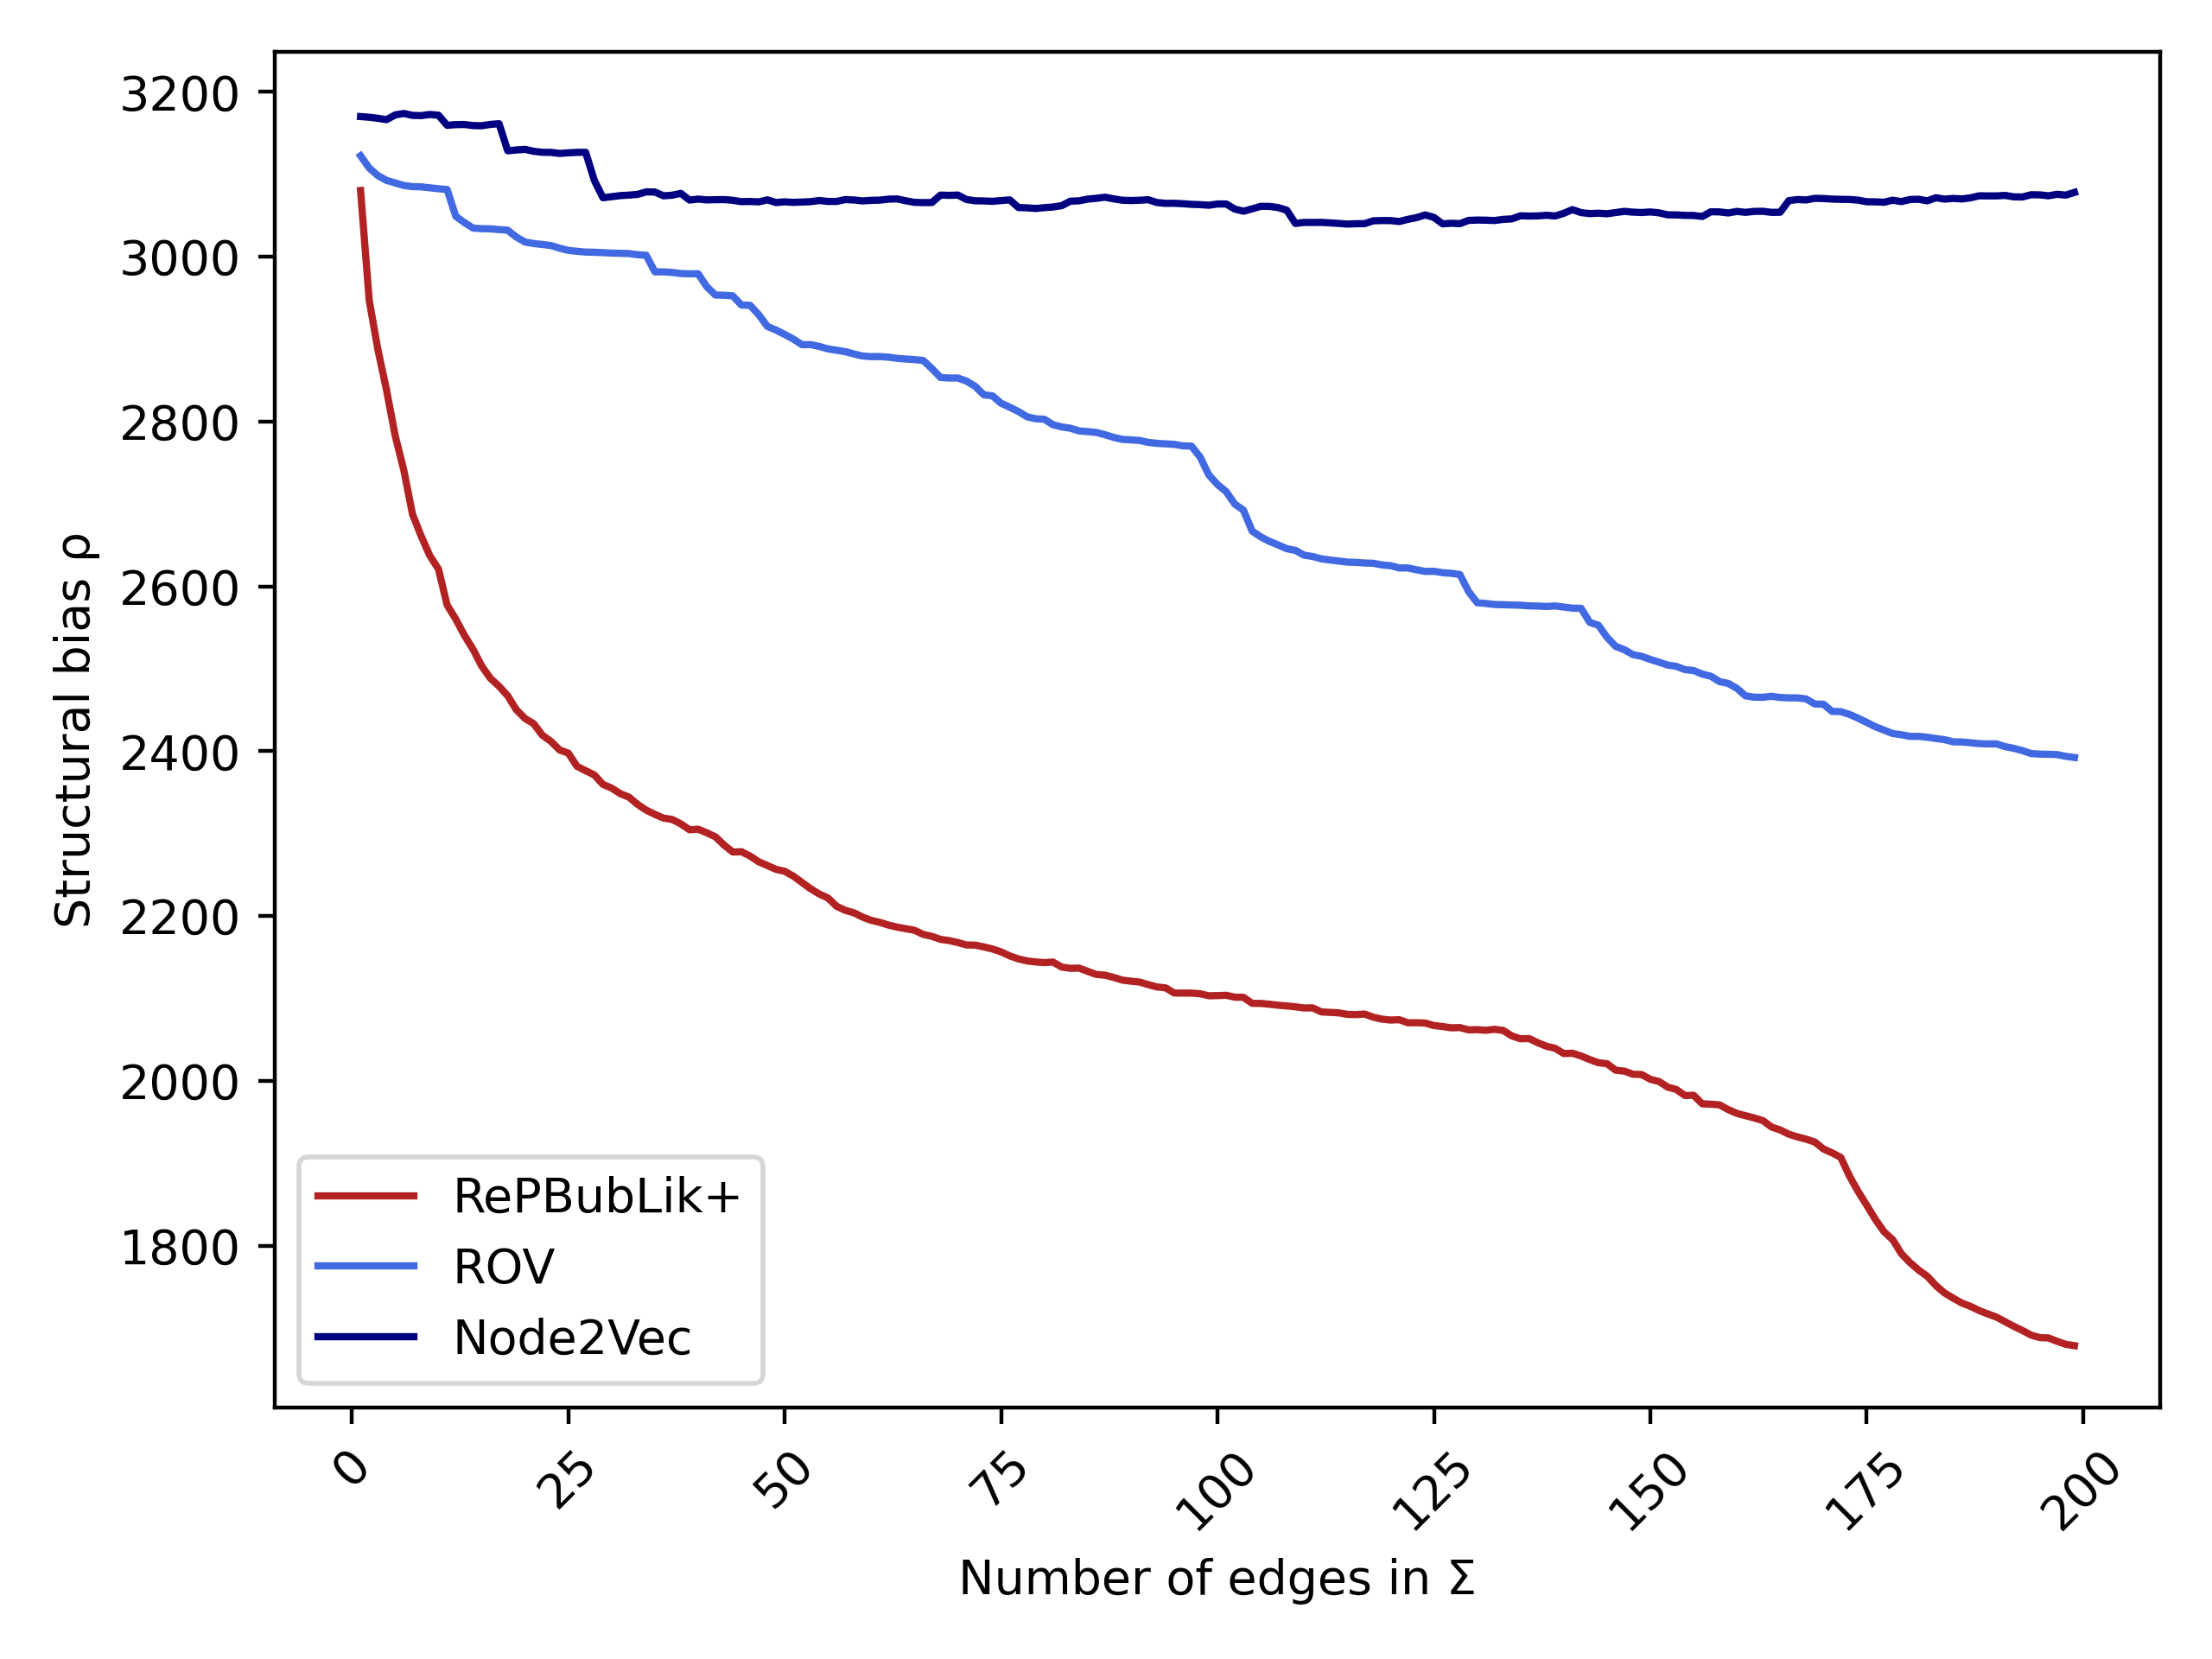
\includegraphics[width=\columnwidth]{15/polblogs_bias_15.png}
    \caption{\emph{PolBlogs} plot}\label{fig:polblogs_b_15}
\end{subfigure}
\caption{Grafici $\rho(G)$ per $t=15$}
\end{figure}
Dai grafici dei bias strutturali, si può dedurre che:
\begin{enumerate}
    \item RePBubLik+ è il migliore tra gli algoritmi proposti, in termini di riduzione di bias $\rho(G)$ rispetto al numero di archi in $\Sigma$.
    \item L'applicazione di RePBubLik+ a grafi di piccole dimensioni (\emph{MaTe}, \emph{MaAs}, \emph{MiHi}) porta ad una diminuzione del bias maggiore rispetto a quella ottenuta mediante gli algoritmi ROV e Node2Vec (es. (\emph{MaAs}) $\delta_{\rho_{R+}}=2700-480=2220$, $\delta_{\rho_{ROV}}=2700-2000=700$, ${\delta_{\rho_{Node2Vec}}}=2700-1800=900$ per $t=10$).
    \item L'applicazione di RePBubLik+ a grafi di medie dimensioni (\emph{PolBlogs}) porta ad una diminuzione del bias maggiore rispetto a quella ottenuta mediante gli algoritmi ROV e Node2Vec (es. (\emph{PolBlogs}) $\delta_{\rho_{R+}}=2750-1500=1250$, $\delta_{\rho_{ROV}}=2750-2250=500$, ${\delta_{\rho_{Node2Vec}}}=2750-2700=50$ per $t=10$).
    \item RePBubLik+ risulta essere il miglior algoritmo in quanto per un numero ridotto di archi riporta una notevole diminuzione del bias: nei grafici sovrastanti, la curva dell'algoritmo RePBubLik+ diminuisce molto rapidamente per valori piccoli di $k$, raggiungendo una plateau per un certo valore di $\rho(G)$.
            Questo, dal punto di vista pratico, è molto interessante perchè permette con pochi archi aggiuntivi di aumentare notevolmente la navigabilità in grafi simili a quelli presi in esame (es. (\emph{MaTe}) $\delta_{\rho_{R+}}=2300-760=1540$, $\delta_{\rho_{ROV}}=2300-2200=100$, ${\delta_{\rho_{Node2Vec}}}=2300-1900=400$ per $k=50,t=10$).
    \item Le considerazioni fatte nei punti precedenti sono generalmente valide, per qualsiasi valore di $t$ e qualsiasi grafo. Valutando il bias strutturale dei grafi anche in termini di RW massimo, si può notare che per valori di $t$ maggiori, RePBubLik+ raggiunge il plateau con un numero inferiore d'archi (es. (\emph{MaTe}) $\delta_{\rho_{R+}}=1350-675=675$ per $k=50, t=5$,  $\delta_{\rho_{R+}}=2300-760=1540$ per $k=50,t=10$, $\delta_{\rho_{R+}}=3400-800=2600$ per $k=50,t=15$).
\end{enumerate}

\subsection{Conclusioni}
Considerando tutti i dati ottenuti dagli esperimenti svolti, RePBubLik+ risulta essere il miglior algoritmo in termini di rapporto tra guadagno e tempo impiegato.
Le performance di quest'ultimo, infatti, variano notevolmente a seconda dei parametri forniti: per valori di $t$ maggiori, 
il guadagno, e la conseguente diminuzione del bias strutturale, aumentano significativamente, a discapito dei tempi di esecuzione. 
Sarebbe utile, quindi, determinare quale lunghezza massima di RW meglio si addice ad un determinato grafo e quanto sia importante la diminuzione della polarizzazione in quella rete.
Per valutare al meglio le performance di RePBubLik+, un'analisi su dataset di dimensioni notevolmente maggiori permetterebbe di esaminare quanto il volume della rete
influenzi le performance dell'algoritmo. 



